\documentclass[12pt]{article}\usepackage[]{graphicx}\usepackage[]{xcolor}
% maxwidth is the original width if it is less than linewidth
% otherwise use linewidth (to make sure the graphics do not exceed the margin)
\makeatletter
\def\maxwidth{ %
  \ifdim\Gin@nat@width>\linewidth
    \linewidth
  \else
    \Gin@nat@width
  \fi
}
\makeatother

\definecolor{fgcolor}{rgb}{0.345, 0.345, 0.345}
\newcommand{\hlnum}[1]{\textcolor[rgb]{0.686,0.059,0.569}{#1}}%
\newcommand{\hlstr}[1]{\textcolor[rgb]{0.192,0.494,0.8}{#1}}%
\newcommand{\hlcom}[1]{\textcolor[rgb]{0.678,0.584,0.686}{\textit{#1}}}%
\newcommand{\hlopt}[1]{\textcolor[rgb]{0,0,0}{#1}}%
\newcommand{\hlstd}[1]{\textcolor[rgb]{0.345,0.345,0.345}{#1}}%
\newcommand{\hlkwa}[1]{\textcolor[rgb]{0.161,0.373,0.58}{\textbf{#1}}}%
\newcommand{\hlkwb}[1]{\textcolor[rgb]{0.69,0.353,0.396}{#1}}%
\newcommand{\hlkwc}[1]{\textcolor[rgb]{0.333,0.667,0.333}{#1}}%
\newcommand{\hlkwd}[1]{\textcolor[rgb]{0.737,0.353,0.396}{\textbf{#1}}}%
\let\hlipl\hlkwb

\usepackage{framed}
\makeatletter
\newenvironment{kframe}{%
 \def\at@end@of@kframe{}%
 \ifinner\ifhmode%
  \def\at@end@of@kframe{\end{minipage}}%
  \begin{minipage}{\columnwidth}%
 \fi\fi%
 \def\FrameCommand##1{\hskip\@totalleftmargin \hskip-\fboxsep
 \colorbox{shadecolor}{##1}\hskip-\fboxsep
     % There is no \\@totalrightmargin, so:
     \hskip-\linewidth \hskip-\@totalleftmargin \hskip\columnwidth}%
 \MakeFramed {\advance\hsize-\width
   \@totalleftmargin\z@ \linewidth\hsize
   \@setminipage}}%
 {\par\unskip\endMakeFramed%
 \at@end@of@kframe}
\makeatother

\definecolor{shadecolor}{rgb}{.97, .97, .97}
\definecolor{messagecolor}{rgb}{0, 0, 0}
\definecolor{warningcolor}{rgb}{1, 0, 1}
\definecolor{errorcolor}{rgb}{1, 0, 0}
\newenvironment{knitrout}{}{} % an empty environment to be redefined in TeX

\usepackage{alltt}    % For submission



%% Package imports %%%%%%%%%%%%%%%%%%%%%%%%%%%%%%%%%%%%%%%%%%%

\usepackage{amsfonts}           % For access to \checkmark.
\usepackage{amsmath}            % For better symbol decorations
\usepackage{authblk}            % For a nice author block
\usepackage{booktabs}           % For nice table rules
\usepackage[official]{eurosym}  % For the euro symbol
\usepackage[figurename=Fig.]{caption} % For changing "Figure" to "Fig." in figure captions
\usepackage{chngcntr}           % To get figure and table numbering correct in the appendices
\usepackage[makeroom]{cancel}   % To show terms go to zero
\usepackage[inline]{enumitem}   % For inline enumeration
\usepackage[letterpaper, left=0.75in, right=0.75in, top=0.75in, bottom=0.75in, footskip=.25in]{geometry} % For better margins.
\usepackage[]{lineno}           % For line numbers
% \modulolinenumbers[5]
\usepackage{microtype}          % For beautiful typesetting
\usepackage{multicol}           % For multi-column layout
\usepackage{multirow}           % For multi-row layout
\usepackage{natbib}
\setlength{\bibsep}{0.0pt}      % To set the separation between entries to 0.
\usepackage{nccmath}            % For the \useshortskip command above equations
\usepackage{parcolumns}         % For multi-column layout
\usepackage{pdflscape}          % For landscape environment \begin{landscape} ... \end{landscape}
\usepackage{setspace}           % For double spacing
\doublespacing
\usepackage{soul}               % For text highlighting
\usepackage[most]{tcolorbox}    % For color highlighting of text
\usepackage{tikz}               % For diagrams
\usetikzlibrary{arrows,positioning}
\usepackage{ulem}               % For strikeout command (\sout)
\usepackage{xcolor}             % For ... colors
\usepackage{xr}                 % For external references to the framework paper
\externaldocument[PartI-]{HSB_framework}

\usepackage{hyperref}           % hyperref should be the last package loaded


%% Macros defined by authors %%%%%%%%%%%%%%%%%%%%%%%%%%%%%%%%%

% The next command tells RStudio to do "Compile PDF" on HSB_framework.Rnw,
% instead of this file, thereby eliminating the need to switch back to HSB_framework.Rnw 
% before building the paper.
%!TEX root = ../HSB_framework.Rnw


%%%%%%%%%%%%%%%%%%%%%%%%%%%%%%%%%%%%%%%%%%%%%%%%%%%%%%%%%%%%%%
% This file contains macros for
% Heun, Semieniuk, Brockway, 
% Energy, expenditure, and consumption aspects of rebound,\\
% Part I: A rigorous analytical framework
% and
% Energy, expenditure, and consumption aspects of rebound,\\
% Part II: Applications of the framework
% 
% It is incorporated into the main file by the command
% % The next command tells RStudio to do "Compile PDF" on HSB_framework.Rnw,
% instead of this file, thereby eliminating the need to switch back to HSB_framework.Rnw 
% before building the paper.
%!TEX root = ../HSB_framework.Rnw


%%%%%%%%%%%%%%%%%%%%%%%%%%%%%%%%%%%%%%%%%%%%%%%%%%%%%%%%%%%%%%
% This file contains macros for
% Heun, Semieniuk, Brockway, 
% Energy, expenditure, and consumption aspects of rebound,\\
% Part I: A rigorous analytical framework
% and
% Energy, expenditure, and consumption aspects of rebound,\\
% Part II: Applications of the framework
% 
% It is incorporated into the main file by the command
% % The next command tells RStudio to do "Compile PDF" on HSB_framework.Rnw,
% instead of this file, thereby eliminating the need to switch back to HSB_framework.Rnw 
% before building the paper.
%!TEX root = ../HSB_framework.Rnw


%%%%%%%%%%%%%%%%%%%%%%%%%%%%%%%%%%%%%%%%%%%%%%%%%%%%%%%%%%%%%%
% This file contains macros for
% Heun, Semieniuk, Brockway, 
% Energy, expenditure, and consumption aspects of rebound,\\
% Part I: A rigorous analytical framework
% and
% Energy, expenditure, and consumption aspects of rebound,\\
% Part II: Applications of the framework
% 
% It is incorporated into the main file by the command
% \input{macros.tex}.
%%%%%%%%%%%%%%%%%%%%%%%%%%%%%%%%%%%%%%%%%%%%%%%%%%%%%%%%%%%%%%


%%%%% Override Energy Economics macros
\renewcommand{\emph}{\textit}


%%%%% Units

\newcommand{\kWhr}{kW$\cdot$hr}
\newcommand{\lmhr}{lm$\cdot$hr}
\newcommand{\passkm}{pass$\cdot$km}
\newcommand{\Whr}{W$\cdot$hr}


%%%%% Decorations for symbols

\newcommand{\rate}[1]{\dot{#1}}                    % Rate of a quantity

% Create "after" commands
\newcommand{\orig}[1]{{}{#1}^{\scriptscriptstyle \circ}}
\newcommand{\aempl}[1]{{#1}^*}
\newcommand{\asub}[1]{\hat{#1}}
\newcommand{\ainc}[1]{\bar{#1}}
\newcommand{\amacro}[1]{\tilde{#1}}

% Create the "before" commands
\newcommand{\bempl}[1]{\orig{#1}}
\newcommand{\bsub}[1]{\aempl{#1}}
\newcommand{\binc}[1]{\asub{#1}}
\newcommand{\bmacro}[1]{\ainc{#1}}

% Decoration combinations
% Rates after
\newcommand{\rorig}[1]{\orig{\rate{#1}}}
\newcommand{\raempl}[1]{\aempl{\rate{#1}}}
\newcommand{\rasub}[1]{\asub{\rate{#1}}}
\newcommand{\rainc}[1]{\ainc{\rate{#1}}}
\newcommand{\ramacro}[1]{\amacro{\rate{#1}}}

% Rates before
\newcommand{\rbempl}[1]{\rorig{#1}}
\newcommand{\rbsub}[1]{\raempl{#1}}
\newcommand{\rbinc}[1]{\rasub{#1}}
\newcommand{\rbmacro}[1]{\rainc{#1}}

%%%%% Subscript kerning

\newcommand{\om}{O\!M}
\newcommand{\omd}{O\!M\!d}
\newcommand{\md}{md}
\newcommand{\macro}{macr\!o}
\newcommand{\life}{li\!f\!e}
\newcommand{\EEU}{E\!EU}

%%%%% Expression kerning

\newcommand{\MPC}{M\!PC}


%%%%% Convenient symbols

\newcommand{\Sdot}{\rate{S}_{dev}}
\newcommand{\Mdothatprime}{\rbinc{M}^\prime}


%%%%% Elasticities and income shares

\newcommand{\eqspsUC}{\varepsilon_{\rate{q}_s\!,p_s}}
\newcommand{\eqopsUC}{\varepsilon_{\rate{q}_o\!,p_s}}
\newcommand{\eqspsC}{\varepsilon_{\rate{q}_s\!,p_s\!,c}}
\newcommand{\eqopsC}{\varepsilon_{\rate{q}_o\!,p_s\!,c}}

% originally
\newcommand{\eqspsUCorig}{\varepsilon^\circ_{\rate{q}_s\!,p_s}}
\newcommand{\eqopsUCorig}{\varepsilon^\circ_{\rate{q}_o\!,p_s}}
\newcommand{\eqspsCorig}{\varepsilon^\circ_{\rate{q}_s\!,p_s\!,c}}
\newcommand{\eqopsCorig}{\varepsilon^\circ_{\rate{q}_o\!,p_s\!,c}}
% With hats
\newcommand{\eqspsUChat}{\hat{\varepsilon}_{\rate{q}_s\!,p_s}}
\newcommand{\eqopsUChat}{\hat{\varepsilon}_{\rate{q}_o\!,p_s}}
\newcommand{\eqspsChat}{\hat{\varepsilon}_{\rate{q}_s\!,p_s\!,c}}
\newcommand{\eqopsChat}{\hat{\varepsilon}_{\rate{q}_o\!,p_s\!,c}}

\newcommand{\eqsM}{\varepsilon_{\rate{q}_s\!,\rate{M}}}
\newcommand{\eqoM}{\varepsilon_{\rate{q}_o\!,\rate{M}}}

\newcommand{\fCs}{\bempl{f}_{\rate{C}_s}}
\newcommand{\fCshat}{\asub{f}_{\rate{C}_s}}

\newcommand{\eQEpE}{\varepsilon_{\rate{Q}_E,p_E}}


%%%%% Colors

% Original spectrum colours
% \colorlet{emplcolor}{red!25!white}
% \colorlet{subcolor}{orange!25!white}
% \colorlet{inccolor}{green!25!white}
% \colorlet{macrocolor}{blue!25!white}

% New Viridis "plasma" colours
\definecolor{emplcolor}{HTML}{150789}
\definecolor{subcolor}{HTML}{99149F}
\definecolor{inccolor}{HTML}{E76F5A}
\definecolor{macrocolor}{HTML}{F7E225}



%%%%% Coloration of text background

%
% Inline color box around text
% Arguments:
%   [#1]: background color for the box
%   {#2}: text inside the box
%
\newtcbox{\inlinebox}[1][]{on line, 
colback=#1,
colframe=#1,
before upper={\rule[-2pt]{0pt}{10pt}},
boxrule=1pt,
boxsep=0pt,
left=3pt,
right=3pt,
top=2pt,
bottom=2pt}


%%%%% Colored phrases

% Emplacement effect
\newcommand{\empleffect}{\inlinebox[emplcolor]{\textcolor{white}{emplacement effect}}}
\newcommand{\empleffectadj}{\inlinebox[emplcolor]{\textcolor{white}{emplacement-effect}}}
\newcommand{\Empleffect}{\inlinebox[emplcolor]{\textcolor{white}{Emplacement effect}}}
\newcommand{\EmplEffect}{\inlinebox[emplcolor]{\textcolor{white}{Emplacement Effect}}}

% Substitution effect
\newcommand{\subeffect}{\inlinebox[subcolor]{\textcolor{white}{substitution effect}}}
\newcommand{\subeffectadj}{\inlinebox[subcolor]{\textcolor{white}{substitution-effect}}}
\newcommand{\Subeffect}{\inlinebox[subcolor]{\textcolor{white}{Substitution effect}}}
\newcommand{\SubEffect}{\inlinebox[subcolor]{\textcolor{white}{Substitution Effect}}}

% Income effect
\newcommand{\inceffect}{\inlinebox[inccolor]{\textcolor{black}{income effect}}}
\newcommand{\inceffectadj}{\inlinebox[inccolor]{\textcolor{black}{income-effect}}}
\newcommand{\Inceffect}{\inlinebox[inccolor]{\textcolor{black}{Income effect}}}
\newcommand{\IncEffect}{\inlinebox[inccolor]{\textcolor{black}{Income Effect}}}

% Macro effect
\newcommand{\macroeffect}{\inlinebox[macrocolor]{\textcolor{black}{macro effect}}}
\newcommand{\macroeffectadj}{\inlinebox[macrocolor]{\textcolor{black}{macro-effect}}}
\newcommand{\Macroeffect}{\inlinebox[macrocolor]{\textcolor{black}{Macro effect}}}
\newcommand{\MacroEffect}{\inlinebox[macrocolor]{\textcolor{black}{Macro Effect}}}


%%%%% minipage for assumptions and constraints tables
% Arguments:
%   #1: Width (multiple of \linewidth
%   #2: text inside the minipage
%
\newcommand{\mptable}[2]{\begin{minipage}{#1\linewidth} \useshortskip{} \begin{equation} #2 \end{equation} \end{minipage}}


%%%%% Oft-used references

\newcommand{\Ba}[1]{\citeauthor[#1]{Borenstein:2015aa}}
\newcommand{\Bapp}[1]{\citeauthor[#1]{Borenstein:2015aa}'s \citeyearpar{Borenstein:2015aa}}
\newcommand{\Bp}[1]{\citep[#1]{Borenstein:2015aa}}
\newcommand{\Bt}[1]{\citet[#1]{Borenstein:2015aa}}

\newcommand{\Ta}[1]{\citeauthor[#1]{Thomas:2013aa}}
\newcommand{\Tapp}[1]{\citeauthor[#1]{Thomas:2013aa}'s \citeyearpar{Thomas:2013aa}}
\newcommand{\Tp}[1]{\citep[#1]{Thomas:2013aa, Thomas:2013ab}}
\newcommand{\Tpone}[1]{\citep[#1]{Thomas:2013aa}}
\newcommand{\Tptwo}[1]{\citep[#1]{Thomas:2013ab}}
\newcommand{\Tt}[1]{\citet[#1]{Thomas:2013aa, Thomas:2013ab}}
\newcommand{\Ttone}[1]{\citet[#1]{Thomas:2013aa}}
\newcommand{\Tttwo}[1]{\citet[#1]{Thomas:2013ab}}


%%%%% Derivation pages

% Column widths
\newcommand{\derivtextsize}{\footnotesize}
\newcommand{\derivpageleftcolwidth}{0.11\textwidth}
\newcommand{\derivpageenergycolwidth}{0.6\textwidth}
\newcommand{\derivpagefinancialcolwidth}{0.6\textwidth}

% Horizontal rule between sections of derivations

\newcommand{\sectionsep}{\noindent\rule{1.4\textwidth}{0.4pt}}


%
% Derivation section
% Arguments:
%   #1: accounting stage (original, prime, etc.)
%   #2: energy column
%   #3: financial column
%
\newcommand{\derivsection}[3]{%

\derivtextsize{}

\begin{minipage}[t]{\derivpageleftcolwidth}
~\\#1
\end{minipage}
%
%
%
\begin{minipage}[t]{\derivpageenergycolwidth}
#2
\end{minipage}
%
~
%
\begin{minipage}[t]{\derivpagefinancialcolwidth}
#3
\end{minipage}

\normalsize{}

}


%
% Derivation page header
% Arguments:
%   #1: Effect type header text (e.g., Emplacement Effect)
%
\newcommand{\derivheader}[1]{

\begin{center}
  #1
\end{center}

\derivsection{}
{\begin{center}\emph{Energy analysis}\end{center}}
{\begin{center}\emph{Financial analysis}\end{center}}

}


% Equations

% Efficiency ratios
\newcommand{\etaratioinline}{\amacro{\eta}/\bempl{\eta}}
\newcommand{\etaratiostacked}{\frac{\amacro{\eta}}{\bempl{\eta}}}

% Derivative with respect to efficiency ratio
\newcommand{\dbydetaeta}{\frac{\mathrm{d}}{\mathrm{d}(\etaratioinline{})}}


% Original
\newcommand{\Eacctorig}{\rbempl{E} = \rbempl{E}_s + \rbempl{E}_{emb} + (\rbempl{C}_{\omd} + \rbempl{C}_o) I_E}
\newcommand{\Macctorig}{\rate{M} = p_E \rbempl{E}_s + \bempl{R}_\alpha \rbempl{C}_{cap} + \rbempl{C}_{\omd} + \rbempl{C}_o + \rbempl{N}}

% Before emplacement effect (same as original)
\newcommand{\Eacctbempl}{\Eacctorig}      
\newcommand{\Macctbempl}{\Macctorig}      

% After emplacement effect
\newcommand{\Eacctaempl}{\raempl{E} = \raempl{E}_s + \raempl{E}_{emb} + (\raempl{C}_{\omd} + \raempl{C}_o) I_E}                  
\newcommand{\Macctaempl}{\rate{M} = p_E \raempl{E}_s + \aempl{R}_\alpha \raempl{C}_{cap} + \raempl{C}_{\omd} + \raempl{C}_o + \raempl{N}}         

% Before substitution effect (same as after emplacement effect)
\newcommand{\Eacctbsub}{\Eacctaempl}
\newcommand{\Macctbsub}{\Macctaempl}

% After substitution effect
\newcommand{\Eacctasub}{\rasub{E} = \rasub{E}_s + \rasub{E}_{emb} + (\rasub{C}_{\omd} + \rasub{C}_o) I_E}
\newcommand{\Macctasub}{\rate{M} = p_E \rasub{E}_s + \asub{R}_\alpha \rasub{C}_{cap} + \rasub{C}_{\omd} + \rasub{C}_o + \rasub{N}}

% Before income effect (same as after substitution effect)
\newcommand{\Eacctbinc}{\Eacctasub}
\newcommand{\Macctbinc}{\Macctasub}

% After income effect
\newcommand{\Eacctainc}{\rainc{E} = \rainc{E}_s + \rainc{E}_{emb} + (\rainc{C}_{\omd} + \rainc{C}_o) I_E}
\newcommand{\Macctainc}{\rate{M} = p_E \rainc{E}_s + \ainc{R}_\alpha \rainc{C}_{cap} + \rainc{C}_{\omd} + \rainc{C}_o + \rainc{N}}

% Embodied energy rebound
\newcommand{\Reembeqn}{\frac{\left( \frac{\aempl{E}_{emb}}{\bempl{E}_{emb}}
  \frac{\bempl{t}_{\life}}{\aempl{t}_{\life}} - 1 \right) \rbempl{E}_{emb}}{\Sdot}}
  
% Ops, Maintenance, and disposal energy rebound
\newcommand{\ReOMdeqn}{\frac{\left( \frac{\raempl{C}_{\omd}}{\rbempl{C}_{\omd}} - 1 \right) \rbempl{C}_{\omd} I_E}{\Sdot}}

% Equation for S_dot_dev
% \newcommand{\Sdoteqn}{\left( \etaratiostacked - 1 \right)\!\etaratiostacked \rbempl{E}_s}
\newcommand{\Sdoteqn}{\left( \etaratiostacked - 1 \right)\! 
                            \frac{\bempl{\eta}}{\amacro{\eta}} \rbempl{E}_s}

% Equation for Re_dsub
\newcommand{\Redsubeqn}{\frac{\left( \etaratiostacked \right)^{-\eqspsUC} - 1}
                        {\etaratiostacked - 1}}
                        
% Equation for Re_isub
\newcommand{\Reisubeqn}{\frac{{\left( \etaratiostacked  \right)}
                          ^{-\eqopsC} - 1}{\etaratiostacked - 1} \; 
                          \etaratiostacked \; 
                          \frac{\rbempl{C}_o I_E}{\rbempl{E}_s}}
                          
% CES utility equation
\newcommand{\cesutility}{\left[ \fCs \left( \frac{\rate{q}_s}{\rbempl{q}_s} \right)^\rho 
        + (1-\fCs) \left( \frac{\rate{C}_o}{\rbempl{C}_o} \right)^\rho  \right]^{(1/\rho)}}
        
% Equation for q_s_hat/q_s_orig
\newcommand{\qssolution}{\left\{ \fCs + (1-\fCs)
      \left[ \left(  \frac{1-\fCs}{\fCs}  \right) \frac{\amacro{p}_s \rbempl{q}_s}{\rbempl{C}_o}  \right]
                                                  ^{\rho / (1 - \rho)} \right\} ^ {-1/\rho}}

% Equation for C_o_hat/C_o_orig
\newcommand{\Cosolution}{ \left( 1 + \fCs \left\{ \left[ \left( \frac{1-\fCs}{\fCs} \right)
          \frac{\amacro{p}_s \rbempl{q}_s}{\rbempl{C}_o} \right] ^{\rho/(\rho - 1)} - 1 \right\} \right)^{-1/\rho}}

% Equation for Re_dsub for the CES utility model
\newcommand{\RedsubCES}{\frac{\qssolution{} - 1}{\etaratiostacked{} - 1}}

% Equation for Re_isub for the CES utility model
\newcommand{\ReisubCES}{\frac{\Cosolution{} - 1}{\etaratiostacked{} - 1}
                         \etaratiostacked \; 
                          \frac{\rbempl{C}_o I_E}{\rbempl{E}_s}}


% Equation for Re_dinc, approximate method
\newcommand{\Redinceqnapprox}{\frac{ \left( 1 + \frac{\rbinc{N}}{\Mdothatprime} \right) ^{\eqsM} - 1}
              { \etaratiostacked - 1 } \left( \etaratiostacked \right)^{-\eqspsC}}

% Equation for Re_dinc, exact method
\newcommand{\Redinceqnexact}{\frac{ \left( 1 + \frac{\rbinc{N}}{\Mdothatprime} \right) ^{\eqsM} - 1}
              { \etaratiostacked - 1 } \qssolution{} }

% Equation for Re_cap
\newcommand{\Recapeqn}{\frac{\Delta \aempl{(R_\alpha \rate{C}_{cap})} I_E}{\Sdot}}

% Equation for Re_iinc, approximate method
\newcommand{\Reiinceqnapprox}{\frac{\left( 1 + \frac{\rbinc{N}}{\Mdothatprime} \right)^{\eqoM} - 1}{\etaratiostacked - 1} 
              \left( \etaratiostacked \right)^{1 - \eqopsC}
              \frac{\rbempl{C}_o I_E}{\rbempl{E}_s}}

% Equation for Re_iinc, exact method
% \newcommand{\Reiinceqnexact}{\frac{\left( 1 + \frac{\rbinc{N}}{\Mdothatprime} \right)^{\eqoM} - 1}{\etaratiostacked - 1} 
%               \left( \etaratiostacked \right)
%               \left( \frac{\rasub{C}_o}{\rorig{C}_o} \right) 
%               \frac{\rbempl{C}_o I_E}{\rbempl{E}_s}}

\newcommand{\Reiinceqnexact}{\frac{\left( 1 + \frac{\rbinc{N}}{\Mdothatprime} \right)^{\eqoM} - 1}{\etaratiostacked - 1} 
              \left( \etaratiostacked \right)
              \frac{\rbempl{C}_o I_E}{\rbempl{E}_s}
              \Cosolution{}}



% Equation for Re_d (total direct rebound)
\newcommand{\Redeqn}{\frac{ \left( \etaratiostacked \right)^{-\eqspsC}
             \left( 1 + \frac{\rasub{N}}{\rbempl{M}} \right)^{\eqsM}   - 1}
         {\etaratiostacked - 1}}

% Equation for Re_macro
% \newcommand{\Remacroeqn}{k (p_E I_E - Re_{cap} - Re_{\md} - p_E I_E Re_{dsub} - Re_{isub})}
\newcommand{\Remacroeqn}{k (p_E I_E - Re_{cap} - Re_{\omd})}

% Equation for Re_tot
% \newcommand{\Retoteqn}{&Re_{emb} - k Re_{cap} + (1-k) Re_{\md}         \nonumber \\
%                        &+ (1 - k p_E I_E) Re_{dsub} + (1 - k) Re_{isub}   \nonumber \\
%                        &+ Re_{dinc} + Re_{iinc} +  k p_E I_E}
% \newcommand{\Retoteqn}{&Re_{emb} + k (p_E I_E - Re_{cap}) + (1-k) Re_{\md}   \nonumber \\
%                        &+ Re_{dsub} + Re_{isub}                              \nonumber \\
%                        &+ Re_{dinc} + Re_{iinc}}
\newcommand{\Retoteqn}{Re_{emb} + k (p_E I_E - Re_{cap}) + (1-k) Re_{\omd} + Re_{dsub} + Re_{isub} + Re_{dinc} + Re_{iinc}}
                 

%%%% Income preference equations

% Equation for energy service income preferences
\newcommand{\incprefseqn}{\frac{\rainc{q}_s}{\rbinc{q}_s} = \left( 1 + \frac{\rbinc{N}}{\Mdothatprime}  \right) ^{\eqsM}}

% Equation for other goods income preferences
\newcommand{\incprefoeqn}{\frac{\rainc{q}_o}{\rbinc{q}_o} = \left( 1 + \frac{\rbinc{N}}{\Mdothatprime}  \right) ^{\eqoM}}

% Equation for effective income
% \newcommand{\effinceqn}{\Mdothatprime \equiv \rbempl{M} - \rbempl{C}_{cap} - \rbempl{C}_{\md} 
%                         - \rate{G} + p_E \Delta \rbinc{E}_s + \Delta \rbinc{C}_o}
\newcommand{\effinceqn}{\Mdothatprime \equiv \rate{M} - \aempl{R}_\alpha \raempl{C}_{cap} - \raempl{C}_{\omd} - \rasub{N}}


%%%% Budget constraint symbols and equation

\newcommand{\tlife}{t_{li\!f\!e}}
\newcommand{\oneyr}{1\,\mathrm{yr}}
\newcommand{\twoyr}{2\,\mathrm{yr}}
\newcommand{\itlife}{i\,t_{li\!f\!e}}
\newcommand{\iyr}{i\,\mathrm{yr}}

\newcommand{\budgetconstraint}{\rate{M} - \orig{R}_\alpha \rorig{C}_{cap} - \rorig{C}_{\omd} = \orig{p}_E \frac{\rorig{q}_s}{\orig{\eta}} + p_o \rorig{q}_o}


%%%% Proof characters
% Equal sign with question mark above
\DeclareRobustCommand{\questionequal}{\stackrel{?}{=}}




% Segments and lines
% Arguments:
%   #1: left character
%   #2: line color
%   #3: line thickness (e.g., 0.1 mm)
%   #4: right character
% Note that \raisebox{0.9 mm} moves the line up from the baseline.
% Also, \line(1,0){12} gives a horizontal line with length "12" (unknown units!)
% (1, 0) is the slope (1 unit to right, 0 units up).
\newcommand{\seg}[4]{#1\linethickness{#3}\raisebox{0.88 mm}{\textcolor{#2}{\line(1,0){12}}}#4}

% Construction lines
\newcommand{\iicirc}{\seg{$\bempl{\text{i}}$}{black}{0.3 mm}{$\,\bempl{\text{i}}$}}
\newcommand{\iibar}{\seg{$\bmacro{\text{i}}$}{black}{0.3 mm}{$\,\bmacro{\text{i}}$}}
\newcommand{\rr}{\seg{r}{black}{0.1 mm}{r}}
\newcommand{\circcirc}{\seg{$\circ$}{black}{0.1 mm}{$\circ$}}
\newcommand{\starstar}{\seg{$*$}{black}{0.1 mm}{$*$}}
\newcommand{\hathat}{\seg{$\wedge$}{black}{0.1 mm}{$\wedge$}}
\newcommand{\barbar}{\seg{$-\,$}{black}{0.1 mm}{$\, -$}}

% Line segments
\newcommand{\circa}{\seg{$\circ$}{emplcolor}{0.6 mm}{$a$}}
% \newcommand{\ab}{\seg{a}{emplcolor}{0.6 mm}{b}}
\newcommand{\ab}{$a$\tikz[baseline=-0.6ex]\draw [line width=0.6mm,dotted,emplcolor] (0,0) -- (0.45,0);$b$}
\newcommand{\bstar}{\seg{$b\,$}{emplcolor}{0.6 mm}{$*$}}
\newcommand{\starc}{\seg{$*$}{subcolor}{0.6 mm}{$\,c$}}
\newcommand{\chat}{\seg{$c\,$}{subcolor}{0.6 mm}{$\wedge$}}
\newcommand{\hatd}{\seg{$\wedge$}{inccolor}{0.6 mm}{$\,d$}}
\newcommand{\dbar}{\seg{$d$}{inccolor}{0.6 mm}{$\,-$}}
\newcommand{\hatbar}{\seg{$\wedge$}{inccolor}{0.6 mm}{$\,-$}}
\newcommand{\bartilde}{\seg{$- \,$}{macrocolor}{0.6 mm}{$\, \sim$}}


% Rotated text for tables
% See
% https://tex.stackexchange.com/questions/98388/how-to-make-table-with-rotated-table-headers-in-latex/98439#98439
% for details.
\newcommand{\rot}{\rotatebox{90}}


% A "rating" command for filled circles with tikz.
% See 
% https://tex.stackexchange.com/questions/194955/get-partly-filled-circle-symbol-scale-linearly-with-parameter
% for details.
\newcommand{\rating}[2][0.75ex]{%
  \pgfmathsetmacro\th{asin(#2/50-1)}% (theta angle of polar coordinates)
    \tikz{%
      \fill[black] (\th:#1) arc (\th:-180-\th:#1) -- cycle;
      \draw[black, thin, radius=#1] (0,0) circle;
    }%
}.
%%%%%%%%%%%%%%%%%%%%%%%%%%%%%%%%%%%%%%%%%%%%%%%%%%%%%%%%%%%%%%


%%%%% Override Energy Economics macros
\renewcommand{\emph}{\textit}


%%%%% Units

\newcommand{\kWhr}{kW$\cdot$hr}
\newcommand{\lmhr}{lm$\cdot$hr}
\newcommand{\passkm}{pass$\cdot$km}
\newcommand{\Whr}{W$\cdot$hr}


%%%%% Decorations for symbols

\newcommand{\rate}[1]{\dot{#1}}                    % Rate of a quantity

% Create "after" commands
\newcommand{\orig}[1]{{}{#1}^{\scriptscriptstyle \circ}}
\newcommand{\aempl}[1]{{#1}^*}
\newcommand{\asub}[1]{\hat{#1}}
\newcommand{\ainc}[1]{\bar{#1}}
\newcommand{\amacro}[1]{\tilde{#1}}

% Create the "before" commands
\newcommand{\bempl}[1]{\orig{#1}}
\newcommand{\bsub}[1]{\aempl{#1}}
\newcommand{\binc}[1]{\asub{#1}}
\newcommand{\bmacro}[1]{\ainc{#1}}

% Decoration combinations
% Rates after
\newcommand{\rorig}[1]{\orig{\rate{#1}}}
\newcommand{\raempl}[1]{\aempl{\rate{#1}}}
\newcommand{\rasub}[1]{\asub{\rate{#1}}}
\newcommand{\rainc}[1]{\ainc{\rate{#1}}}
\newcommand{\ramacro}[1]{\amacro{\rate{#1}}}

% Rates before
\newcommand{\rbempl}[1]{\rorig{#1}}
\newcommand{\rbsub}[1]{\raempl{#1}}
\newcommand{\rbinc}[1]{\rasub{#1}}
\newcommand{\rbmacro}[1]{\rainc{#1}}

%%%%% Subscript kerning

\newcommand{\om}{O\!M}
\newcommand{\omd}{O\!M\!d}
\newcommand{\md}{md}
\newcommand{\macro}{macr\!o}
\newcommand{\life}{li\!f\!e}
\newcommand{\EEU}{E\!EU}

%%%%% Expression kerning

\newcommand{\MPC}{M\!PC}


%%%%% Convenient symbols

\newcommand{\Sdot}{\rate{S}_{dev}}
\newcommand{\Mdothatprime}{\rbinc{M}^\prime}


%%%%% Elasticities and income shares

\newcommand{\eqspsUC}{\varepsilon_{\rate{q}_s\!,p_s}}
\newcommand{\eqopsUC}{\varepsilon_{\rate{q}_o\!,p_s}}
\newcommand{\eqspsC}{\varepsilon_{\rate{q}_s\!,p_s\!,c}}
\newcommand{\eqopsC}{\varepsilon_{\rate{q}_o\!,p_s\!,c}}

% originally
\newcommand{\eqspsUCorig}{\varepsilon^\circ_{\rate{q}_s\!,p_s}}
\newcommand{\eqopsUCorig}{\varepsilon^\circ_{\rate{q}_o\!,p_s}}
\newcommand{\eqspsCorig}{\varepsilon^\circ_{\rate{q}_s\!,p_s\!,c}}
\newcommand{\eqopsCorig}{\varepsilon^\circ_{\rate{q}_o\!,p_s\!,c}}
% With hats
\newcommand{\eqspsUChat}{\hat{\varepsilon}_{\rate{q}_s\!,p_s}}
\newcommand{\eqopsUChat}{\hat{\varepsilon}_{\rate{q}_o\!,p_s}}
\newcommand{\eqspsChat}{\hat{\varepsilon}_{\rate{q}_s\!,p_s\!,c}}
\newcommand{\eqopsChat}{\hat{\varepsilon}_{\rate{q}_o\!,p_s\!,c}}

\newcommand{\eqsM}{\varepsilon_{\rate{q}_s\!,\rate{M}}}
\newcommand{\eqoM}{\varepsilon_{\rate{q}_o\!,\rate{M}}}

\newcommand{\fCs}{\bempl{f}_{\rate{C}_s}}
\newcommand{\fCshat}{\asub{f}_{\rate{C}_s}}

\newcommand{\eQEpE}{\varepsilon_{\rate{Q}_E,p_E}}


%%%%% Colors

% Original spectrum colours
% \colorlet{emplcolor}{red!25!white}
% \colorlet{subcolor}{orange!25!white}
% \colorlet{inccolor}{green!25!white}
% \colorlet{macrocolor}{blue!25!white}

% New Viridis "plasma" colours
\definecolor{emplcolor}{HTML}{150789}
\definecolor{subcolor}{HTML}{99149F}
\definecolor{inccolor}{HTML}{E76F5A}
\definecolor{macrocolor}{HTML}{F7E225}



%%%%% Coloration of text background

%
% Inline color box around text
% Arguments:
%   [#1]: background color for the box
%   {#2}: text inside the box
%
\newtcbox{\inlinebox}[1][]{on line, 
colback=#1,
colframe=#1,
before upper={\rule[-2pt]{0pt}{10pt}},
boxrule=1pt,
boxsep=0pt,
left=3pt,
right=3pt,
top=2pt,
bottom=2pt}


%%%%% Colored phrases

% Emplacement effect
\newcommand{\empleffect}{\inlinebox[emplcolor]{\textcolor{white}{emplacement effect}}}
\newcommand{\empleffectadj}{\inlinebox[emplcolor]{\textcolor{white}{emplacement-effect}}}
\newcommand{\Empleffect}{\inlinebox[emplcolor]{\textcolor{white}{Emplacement effect}}}
\newcommand{\EmplEffect}{\inlinebox[emplcolor]{\textcolor{white}{Emplacement Effect}}}

% Substitution effect
\newcommand{\subeffect}{\inlinebox[subcolor]{\textcolor{white}{substitution effect}}}
\newcommand{\subeffectadj}{\inlinebox[subcolor]{\textcolor{white}{substitution-effect}}}
\newcommand{\Subeffect}{\inlinebox[subcolor]{\textcolor{white}{Substitution effect}}}
\newcommand{\SubEffect}{\inlinebox[subcolor]{\textcolor{white}{Substitution Effect}}}

% Income effect
\newcommand{\inceffect}{\inlinebox[inccolor]{\textcolor{black}{income effect}}}
\newcommand{\inceffectadj}{\inlinebox[inccolor]{\textcolor{black}{income-effect}}}
\newcommand{\Inceffect}{\inlinebox[inccolor]{\textcolor{black}{Income effect}}}
\newcommand{\IncEffect}{\inlinebox[inccolor]{\textcolor{black}{Income Effect}}}

% Macro effect
\newcommand{\macroeffect}{\inlinebox[macrocolor]{\textcolor{black}{macro effect}}}
\newcommand{\macroeffectadj}{\inlinebox[macrocolor]{\textcolor{black}{macro-effect}}}
\newcommand{\Macroeffect}{\inlinebox[macrocolor]{\textcolor{black}{Macro effect}}}
\newcommand{\MacroEffect}{\inlinebox[macrocolor]{\textcolor{black}{Macro Effect}}}


%%%%% minipage for assumptions and constraints tables
% Arguments:
%   #1: Width (multiple of \linewidth
%   #2: text inside the minipage
%
\newcommand{\mptable}[2]{\begin{minipage}{#1\linewidth} \useshortskip{} \begin{equation} #2 \end{equation} \end{minipage}}


%%%%% Oft-used references

\newcommand{\Ba}[1]{\citeauthor[#1]{Borenstein:2015aa}}
\newcommand{\Bapp}[1]{\citeauthor[#1]{Borenstein:2015aa}'s \citeyearpar{Borenstein:2015aa}}
\newcommand{\Bp}[1]{\citep[#1]{Borenstein:2015aa}}
\newcommand{\Bt}[1]{\citet[#1]{Borenstein:2015aa}}

\newcommand{\Ta}[1]{\citeauthor[#1]{Thomas:2013aa}}
\newcommand{\Tapp}[1]{\citeauthor[#1]{Thomas:2013aa}'s \citeyearpar{Thomas:2013aa}}
\newcommand{\Tp}[1]{\citep[#1]{Thomas:2013aa, Thomas:2013ab}}
\newcommand{\Tpone}[1]{\citep[#1]{Thomas:2013aa}}
\newcommand{\Tptwo}[1]{\citep[#1]{Thomas:2013ab}}
\newcommand{\Tt}[1]{\citet[#1]{Thomas:2013aa, Thomas:2013ab}}
\newcommand{\Ttone}[1]{\citet[#1]{Thomas:2013aa}}
\newcommand{\Tttwo}[1]{\citet[#1]{Thomas:2013ab}}


%%%%% Derivation pages

% Column widths
\newcommand{\derivtextsize}{\footnotesize}
\newcommand{\derivpageleftcolwidth}{0.11\textwidth}
\newcommand{\derivpageenergycolwidth}{0.6\textwidth}
\newcommand{\derivpagefinancialcolwidth}{0.6\textwidth}

% Horizontal rule between sections of derivations

\newcommand{\sectionsep}{\noindent\rule{1.4\textwidth}{0.4pt}}


%
% Derivation section
% Arguments:
%   #1: accounting stage (original, prime, etc.)
%   #2: energy column
%   #3: financial column
%
\newcommand{\derivsection}[3]{%

\derivtextsize{}

\begin{minipage}[t]{\derivpageleftcolwidth}
~\\#1
\end{minipage}
%
%
%
\begin{minipage}[t]{\derivpageenergycolwidth}
#2
\end{minipage}
%
~
%
\begin{minipage}[t]{\derivpagefinancialcolwidth}
#3
\end{minipage}

\normalsize{}

}


%
% Derivation page header
% Arguments:
%   #1: Effect type header text (e.g., Emplacement Effect)
%
\newcommand{\derivheader}[1]{

\begin{center}
  #1
\end{center}

\derivsection{}
{\begin{center}\emph{Energy analysis}\end{center}}
{\begin{center}\emph{Financial analysis}\end{center}}

}


% Equations

% Efficiency ratios
\newcommand{\etaratioinline}{\amacro{\eta}/\bempl{\eta}}
\newcommand{\etaratiostacked}{\frac{\amacro{\eta}}{\bempl{\eta}}}

% Derivative with respect to efficiency ratio
\newcommand{\dbydetaeta}{\frac{\mathrm{d}}{\mathrm{d}(\etaratioinline{})}}


% Original
\newcommand{\Eacctorig}{\rbempl{E} = \rbempl{E}_s + \rbempl{E}_{emb} + (\rbempl{C}_{\omd} + \rbempl{C}_o) I_E}
\newcommand{\Macctorig}{\rate{M} = p_E \rbempl{E}_s + \bempl{R}_\alpha \rbempl{C}_{cap} + \rbempl{C}_{\omd} + \rbempl{C}_o + \rbempl{N}}

% Before emplacement effect (same as original)
\newcommand{\Eacctbempl}{\Eacctorig}      
\newcommand{\Macctbempl}{\Macctorig}      

% After emplacement effect
\newcommand{\Eacctaempl}{\raempl{E} = \raempl{E}_s + \raempl{E}_{emb} + (\raempl{C}_{\omd} + \raempl{C}_o) I_E}                  
\newcommand{\Macctaempl}{\rate{M} = p_E \raempl{E}_s + \aempl{R}_\alpha \raempl{C}_{cap} + \raempl{C}_{\omd} + \raempl{C}_o + \raempl{N}}         

% Before substitution effect (same as after emplacement effect)
\newcommand{\Eacctbsub}{\Eacctaempl}
\newcommand{\Macctbsub}{\Macctaempl}

% After substitution effect
\newcommand{\Eacctasub}{\rasub{E} = \rasub{E}_s + \rasub{E}_{emb} + (\rasub{C}_{\omd} + \rasub{C}_o) I_E}
\newcommand{\Macctasub}{\rate{M} = p_E \rasub{E}_s + \asub{R}_\alpha \rasub{C}_{cap} + \rasub{C}_{\omd} + \rasub{C}_o + \rasub{N}}

% Before income effect (same as after substitution effect)
\newcommand{\Eacctbinc}{\Eacctasub}
\newcommand{\Macctbinc}{\Macctasub}

% After income effect
\newcommand{\Eacctainc}{\rainc{E} = \rainc{E}_s + \rainc{E}_{emb} + (\rainc{C}_{\omd} + \rainc{C}_o) I_E}
\newcommand{\Macctainc}{\rate{M} = p_E \rainc{E}_s + \ainc{R}_\alpha \rainc{C}_{cap} + \rainc{C}_{\omd} + \rainc{C}_o + \rainc{N}}

% Embodied energy rebound
\newcommand{\Reembeqn}{\frac{\left( \frac{\aempl{E}_{emb}}{\bempl{E}_{emb}}
  \frac{\bempl{t}_{\life}}{\aempl{t}_{\life}} - 1 \right) \rbempl{E}_{emb}}{\Sdot}}
  
% Ops, Maintenance, and disposal energy rebound
\newcommand{\ReOMdeqn}{\frac{\left( \frac{\raempl{C}_{\omd}}{\rbempl{C}_{\omd}} - 1 \right) \rbempl{C}_{\omd} I_E}{\Sdot}}

% Equation for S_dot_dev
% \newcommand{\Sdoteqn}{\left( \etaratiostacked - 1 \right)\!\etaratiostacked \rbempl{E}_s}
\newcommand{\Sdoteqn}{\left( \etaratiostacked - 1 \right)\! 
                            \frac{\bempl{\eta}}{\amacro{\eta}} \rbempl{E}_s}

% Equation for Re_dsub
\newcommand{\Redsubeqn}{\frac{\left( \etaratiostacked \right)^{-\eqspsUC} - 1}
                        {\etaratiostacked - 1}}
                        
% Equation for Re_isub
\newcommand{\Reisubeqn}{\frac{{\left( \etaratiostacked  \right)}
                          ^{-\eqopsC} - 1}{\etaratiostacked - 1} \; 
                          \etaratiostacked \; 
                          \frac{\rbempl{C}_o I_E}{\rbempl{E}_s}}
                          
% CES utility equation
\newcommand{\cesutility}{\left[ \fCs \left( \frac{\rate{q}_s}{\rbempl{q}_s} \right)^\rho 
        + (1-\fCs) \left( \frac{\rate{C}_o}{\rbempl{C}_o} \right)^\rho  \right]^{(1/\rho)}}
        
% Equation for q_s_hat/q_s_orig
\newcommand{\qssolution}{\left\{ \fCs + (1-\fCs)
      \left[ \left(  \frac{1-\fCs}{\fCs}  \right) \frac{\amacro{p}_s \rbempl{q}_s}{\rbempl{C}_o}  \right]
                                                  ^{\rho / (1 - \rho)} \right\} ^ {-1/\rho}}

% Equation for C_o_hat/C_o_orig
\newcommand{\Cosolution}{ \left( 1 + \fCs \left\{ \left[ \left( \frac{1-\fCs}{\fCs} \right)
          \frac{\amacro{p}_s \rbempl{q}_s}{\rbempl{C}_o} \right] ^{\rho/(\rho - 1)} - 1 \right\} \right)^{-1/\rho}}

% Equation for Re_dsub for the CES utility model
\newcommand{\RedsubCES}{\frac{\qssolution{} - 1}{\etaratiostacked{} - 1}}

% Equation for Re_isub for the CES utility model
\newcommand{\ReisubCES}{\frac{\Cosolution{} - 1}{\etaratiostacked{} - 1}
                         \etaratiostacked \; 
                          \frac{\rbempl{C}_o I_E}{\rbempl{E}_s}}


% Equation for Re_dinc, approximate method
\newcommand{\Redinceqnapprox}{\frac{ \left( 1 + \frac{\rbinc{N}}{\Mdothatprime} \right) ^{\eqsM} - 1}
              { \etaratiostacked - 1 } \left( \etaratiostacked \right)^{-\eqspsC}}

% Equation for Re_dinc, exact method
\newcommand{\Redinceqnexact}{\frac{ \left( 1 + \frac{\rbinc{N}}{\Mdothatprime} \right) ^{\eqsM} - 1}
              { \etaratiostacked - 1 } \qssolution{} }

% Equation for Re_cap
\newcommand{\Recapeqn}{\frac{\Delta \aempl{(R_\alpha \rate{C}_{cap})} I_E}{\Sdot}}

% Equation for Re_iinc, approximate method
\newcommand{\Reiinceqnapprox}{\frac{\left( 1 + \frac{\rbinc{N}}{\Mdothatprime} \right)^{\eqoM} - 1}{\etaratiostacked - 1} 
              \left( \etaratiostacked \right)^{1 - \eqopsC}
              \frac{\rbempl{C}_o I_E}{\rbempl{E}_s}}

% Equation for Re_iinc, exact method
% \newcommand{\Reiinceqnexact}{\frac{\left( 1 + \frac{\rbinc{N}}{\Mdothatprime} \right)^{\eqoM} - 1}{\etaratiostacked - 1} 
%               \left( \etaratiostacked \right)
%               \left( \frac{\rasub{C}_o}{\rorig{C}_o} \right) 
%               \frac{\rbempl{C}_o I_E}{\rbempl{E}_s}}

\newcommand{\Reiinceqnexact}{\frac{\left( 1 + \frac{\rbinc{N}}{\Mdothatprime} \right)^{\eqoM} - 1}{\etaratiostacked - 1} 
              \left( \etaratiostacked \right)
              \frac{\rbempl{C}_o I_E}{\rbempl{E}_s}
              \Cosolution{}}



% Equation for Re_d (total direct rebound)
\newcommand{\Redeqn}{\frac{ \left( \etaratiostacked \right)^{-\eqspsC}
             \left( 1 + \frac{\rasub{N}}{\rbempl{M}} \right)^{\eqsM}   - 1}
         {\etaratiostacked - 1}}

% Equation for Re_macro
% \newcommand{\Remacroeqn}{k (p_E I_E - Re_{cap} - Re_{\md} - p_E I_E Re_{dsub} - Re_{isub})}
\newcommand{\Remacroeqn}{k (p_E I_E - Re_{cap} - Re_{\omd})}

% Equation for Re_tot
% \newcommand{\Retoteqn}{&Re_{emb} - k Re_{cap} + (1-k) Re_{\md}         \nonumber \\
%                        &+ (1 - k p_E I_E) Re_{dsub} + (1 - k) Re_{isub}   \nonumber \\
%                        &+ Re_{dinc} + Re_{iinc} +  k p_E I_E}
% \newcommand{\Retoteqn}{&Re_{emb} + k (p_E I_E - Re_{cap}) + (1-k) Re_{\md}   \nonumber \\
%                        &+ Re_{dsub} + Re_{isub}                              \nonumber \\
%                        &+ Re_{dinc} + Re_{iinc}}
\newcommand{\Retoteqn}{Re_{emb} + k (p_E I_E - Re_{cap}) + (1-k) Re_{\omd} + Re_{dsub} + Re_{isub} + Re_{dinc} + Re_{iinc}}
                 

%%%% Income preference equations

% Equation for energy service income preferences
\newcommand{\incprefseqn}{\frac{\rainc{q}_s}{\rbinc{q}_s} = \left( 1 + \frac{\rbinc{N}}{\Mdothatprime}  \right) ^{\eqsM}}

% Equation for other goods income preferences
\newcommand{\incprefoeqn}{\frac{\rainc{q}_o}{\rbinc{q}_o} = \left( 1 + \frac{\rbinc{N}}{\Mdothatprime}  \right) ^{\eqoM}}

% Equation for effective income
% \newcommand{\effinceqn}{\Mdothatprime \equiv \rbempl{M} - \rbempl{C}_{cap} - \rbempl{C}_{\md} 
%                         - \rate{G} + p_E \Delta \rbinc{E}_s + \Delta \rbinc{C}_o}
\newcommand{\effinceqn}{\Mdothatprime \equiv \rate{M} - \aempl{R}_\alpha \raempl{C}_{cap} - \raempl{C}_{\omd} - \rasub{N}}


%%%% Budget constraint symbols and equation

\newcommand{\tlife}{t_{li\!f\!e}}
\newcommand{\oneyr}{1\,\mathrm{yr}}
\newcommand{\twoyr}{2\,\mathrm{yr}}
\newcommand{\itlife}{i\,t_{li\!f\!e}}
\newcommand{\iyr}{i\,\mathrm{yr}}

\newcommand{\budgetconstraint}{\rate{M} - \orig{R}_\alpha \rorig{C}_{cap} - \rorig{C}_{\omd} = \orig{p}_E \frac{\rorig{q}_s}{\orig{\eta}} + p_o \rorig{q}_o}


%%%% Proof characters
% Equal sign with question mark above
\DeclareRobustCommand{\questionequal}{\stackrel{?}{=}}




% Segments and lines
% Arguments:
%   #1: left character
%   #2: line color
%   #3: line thickness (e.g., 0.1 mm)
%   #4: right character
% Note that \raisebox{0.9 mm} moves the line up from the baseline.
% Also, \line(1,0){12} gives a horizontal line with length "12" (unknown units!)
% (1, 0) is the slope (1 unit to right, 0 units up).
\newcommand{\seg}[4]{#1\linethickness{#3}\raisebox{0.88 mm}{\textcolor{#2}{\line(1,0){12}}}#4}

% Construction lines
\newcommand{\iicirc}{\seg{$\bempl{\text{i}}$}{black}{0.3 mm}{$\,\bempl{\text{i}}$}}
\newcommand{\iibar}{\seg{$\bmacro{\text{i}}$}{black}{0.3 mm}{$\,\bmacro{\text{i}}$}}
\newcommand{\rr}{\seg{r}{black}{0.1 mm}{r}}
\newcommand{\circcirc}{\seg{$\circ$}{black}{0.1 mm}{$\circ$}}
\newcommand{\starstar}{\seg{$*$}{black}{0.1 mm}{$*$}}
\newcommand{\hathat}{\seg{$\wedge$}{black}{0.1 mm}{$\wedge$}}
\newcommand{\barbar}{\seg{$-\,$}{black}{0.1 mm}{$\, -$}}

% Line segments
\newcommand{\circa}{\seg{$\circ$}{emplcolor}{0.6 mm}{$a$}}
% \newcommand{\ab}{\seg{a}{emplcolor}{0.6 mm}{b}}
\newcommand{\ab}{$a$\tikz[baseline=-0.6ex]\draw [line width=0.6mm,dotted,emplcolor] (0,0) -- (0.45,0);$b$}
\newcommand{\bstar}{\seg{$b\,$}{emplcolor}{0.6 mm}{$*$}}
\newcommand{\starc}{\seg{$*$}{subcolor}{0.6 mm}{$\,c$}}
\newcommand{\chat}{\seg{$c\,$}{subcolor}{0.6 mm}{$\wedge$}}
\newcommand{\hatd}{\seg{$\wedge$}{inccolor}{0.6 mm}{$\,d$}}
\newcommand{\dbar}{\seg{$d$}{inccolor}{0.6 mm}{$\,-$}}
\newcommand{\hatbar}{\seg{$\wedge$}{inccolor}{0.6 mm}{$\,-$}}
\newcommand{\bartilde}{\seg{$- \,$}{macrocolor}{0.6 mm}{$\, \sim$}}


% Rotated text for tables
% See
% https://tex.stackexchange.com/questions/98388/how-to-make-table-with-rotated-table-headers-in-latex/98439#98439
% for details.
\newcommand{\rot}{\rotatebox{90}}


% A "rating" command for filled circles with tikz.
% See 
% https://tex.stackexchange.com/questions/194955/get-partly-filled-circle-symbol-scale-linearly-with-parameter
% for details.
\newcommand{\rating}[2][0.75ex]{%
  \pgfmathsetmacro\th{asin(#2/50-1)}% (theta angle of polar coordinates)
    \tikz{%
      \fill[black] (\th:#1) arc (\th:-180-\th:#1) -- cycle;
      \draw[black, thin, radius=#1] (0,0) circle;
    }%
}.
%%%%%%%%%%%%%%%%%%%%%%%%%%%%%%%%%%%%%%%%%%%%%%%%%%%%%%%%%%%%%%


%%%%% Override Energy Economics macros
\renewcommand{\emph}{\textit}


%%%%% Units

\newcommand{\kWhr}{kW$\cdot$hr}
\newcommand{\lmhr}{lm$\cdot$hr}
\newcommand{\passkm}{pass$\cdot$km}
\newcommand{\Whr}{W$\cdot$hr}


%%%%% Decorations for symbols

\newcommand{\rate}[1]{\dot{#1}}                    % Rate of a quantity

% Create "after" commands
\newcommand{\orig}[1]{{}{#1}^{\scriptscriptstyle \circ}}
\newcommand{\aempl}[1]{{#1}^*}
\newcommand{\asub}[1]{\hat{#1}}
\newcommand{\ainc}[1]{\bar{#1}}
\newcommand{\amacro}[1]{\tilde{#1}}

% Create the "before" commands
\newcommand{\bempl}[1]{\orig{#1}}
\newcommand{\bsub}[1]{\aempl{#1}}
\newcommand{\binc}[1]{\asub{#1}}
\newcommand{\bmacro}[1]{\ainc{#1}}

% Decoration combinations
% Rates after
\newcommand{\rorig}[1]{\orig{\rate{#1}}}
\newcommand{\raempl}[1]{\aempl{\rate{#1}}}
\newcommand{\rasub}[1]{\asub{\rate{#1}}}
\newcommand{\rainc}[1]{\ainc{\rate{#1}}}
\newcommand{\ramacro}[1]{\amacro{\rate{#1}}}

% Rates before
\newcommand{\rbempl}[1]{\rorig{#1}}
\newcommand{\rbsub}[1]{\raempl{#1}}
\newcommand{\rbinc}[1]{\rasub{#1}}
\newcommand{\rbmacro}[1]{\rainc{#1}}

%%%%% Subscript kerning

\newcommand{\om}{O\!M}
\newcommand{\omd}{O\!M\!d}
\newcommand{\md}{md}
\newcommand{\macro}{macr\!o}
\newcommand{\life}{li\!f\!e}
\newcommand{\EEU}{E\!EU}

%%%%% Expression kerning

\newcommand{\MPC}{M\!PC}


%%%%% Convenient symbols

\newcommand{\Sdot}{\rate{S}_{dev}}
\newcommand{\Mdothatprime}{\rbinc{M}^\prime}


%%%%% Elasticities and income shares

\newcommand{\eqspsUC}{\varepsilon_{\rate{q}_s\!,p_s}}
\newcommand{\eqopsUC}{\varepsilon_{\rate{q}_o\!,p_s}}
\newcommand{\eqspsC}{\varepsilon_{\rate{q}_s\!,p_s\!,c}}
\newcommand{\eqopsC}{\varepsilon_{\rate{q}_o\!,p_s\!,c}}

% originally
\newcommand{\eqspsUCorig}{\varepsilon^\circ_{\rate{q}_s\!,p_s}}
\newcommand{\eqopsUCorig}{\varepsilon^\circ_{\rate{q}_o\!,p_s}}
\newcommand{\eqspsCorig}{\varepsilon^\circ_{\rate{q}_s\!,p_s\!,c}}
\newcommand{\eqopsCorig}{\varepsilon^\circ_{\rate{q}_o\!,p_s\!,c}}
% With hats
\newcommand{\eqspsUChat}{\hat{\varepsilon}_{\rate{q}_s\!,p_s}}
\newcommand{\eqopsUChat}{\hat{\varepsilon}_{\rate{q}_o\!,p_s}}
\newcommand{\eqspsChat}{\hat{\varepsilon}_{\rate{q}_s\!,p_s\!,c}}
\newcommand{\eqopsChat}{\hat{\varepsilon}_{\rate{q}_o\!,p_s\!,c}}

\newcommand{\eqsM}{\varepsilon_{\rate{q}_s\!,\rate{M}}}
\newcommand{\eqoM}{\varepsilon_{\rate{q}_o\!,\rate{M}}}

\newcommand{\fCs}{\bempl{f}_{\rate{C}_s}}
\newcommand{\fCshat}{\asub{f}_{\rate{C}_s}}

\newcommand{\eQEpE}{\varepsilon_{\rate{Q}_E,p_E}}


%%%%% Colors

% Original spectrum colours
% \colorlet{emplcolor}{red!25!white}
% \colorlet{subcolor}{orange!25!white}
% \colorlet{inccolor}{green!25!white}
% \colorlet{macrocolor}{blue!25!white}

% New Viridis "plasma" colours
\definecolor{emplcolor}{HTML}{150789}
\definecolor{subcolor}{HTML}{99149F}
\definecolor{inccolor}{HTML}{E76F5A}
\definecolor{macrocolor}{HTML}{F7E225}



%%%%% Coloration of text background

%
% Inline color box around text
% Arguments:
%   [#1]: background color for the box
%   {#2}: text inside the box
%
\newtcbox{\inlinebox}[1][]{on line, 
colback=#1,
colframe=#1,
before upper={\rule[-2pt]{0pt}{10pt}},
boxrule=1pt,
boxsep=0pt,
left=3pt,
right=3pt,
top=2pt,
bottom=2pt}


%%%%% Colored phrases

% Emplacement effect
\newcommand{\empleffect}{\inlinebox[emplcolor]{\textcolor{white}{emplacement effect}}}
\newcommand{\empleffectadj}{\inlinebox[emplcolor]{\textcolor{white}{emplacement-effect}}}
\newcommand{\Empleffect}{\inlinebox[emplcolor]{\textcolor{white}{Emplacement effect}}}
\newcommand{\EmplEffect}{\inlinebox[emplcolor]{\textcolor{white}{Emplacement Effect}}}

% Substitution effect
\newcommand{\subeffect}{\inlinebox[subcolor]{\textcolor{white}{substitution effect}}}
\newcommand{\subeffectadj}{\inlinebox[subcolor]{\textcolor{white}{substitution-effect}}}
\newcommand{\Subeffect}{\inlinebox[subcolor]{\textcolor{white}{Substitution effect}}}
\newcommand{\SubEffect}{\inlinebox[subcolor]{\textcolor{white}{Substitution Effect}}}

% Income effect
\newcommand{\inceffect}{\inlinebox[inccolor]{\textcolor{black}{income effect}}}
\newcommand{\inceffectadj}{\inlinebox[inccolor]{\textcolor{black}{income-effect}}}
\newcommand{\Inceffect}{\inlinebox[inccolor]{\textcolor{black}{Income effect}}}
\newcommand{\IncEffect}{\inlinebox[inccolor]{\textcolor{black}{Income Effect}}}

% Macro effect
\newcommand{\macroeffect}{\inlinebox[macrocolor]{\textcolor{black}{macro effect}}}
\newcommand{\macroeffectadj}{\inlinebox[macrocolor]{\textcolor{black}{macro-effect}}}
\newcommand{\Macroeffect}{\inlinebox[macrocolor]{\textcolor{black}{Macro effect}}}
\newcommand{\MacroEffect}{\inlinebox[macrocolor]{\textcolor{black}{Macro Effect}}}


%%%%% minipage for assumptions and constraints tables
% Arguments:
%   #1: Width (multiple of \linewidth
%   #2: text inside the minipage
%
\newcommand{\mptable}[2]{\begin{minipage}{#1\linewidth} \useshortskip{} \begin{equation} #2 \end{equation} \end{minipage}}


%%%%% Oft-used references

\newcommand{\Ba}[1]{\citeauthor[#1]{Borenstein:2015aa}}
\newcommand{\Bapp}[1]{\citeauthor[#1]{Borenstein:2015aa}'s \citeyearpar{Borenstein:2015aa}}
\newcommand{\Bp}[1]{\citep[#1]{Borenstein:2015aa}}
\newcommand{\Bt}[1]{\citet[#1]{Borenstein:2015aa}}

\newcommand{\Ta}[1]{\citeauthor[#1]{Thomas:2013aa}}
\newcommand{\Tapp}[1]{\citeauthor[#1]{Thomas:2013aa}'s \citeyearpar{Thomas:2013aa}}
\newcommand{\Tp}[1]{\citep[#1]{Thomas:2013aa, Thomas:2013ab}}
\newcommand{\Tpone}[1]{\citep[#1]{Thomas:2013aa}}
\newcommand{\Tptwo}[1]{\citep[#1]{Thomas:2013ab}}
\newcommand{\Tt}[1]{\citet[#1]{Thomas:2013aa, Thomas:2013ab}}
\newcommand{\Ttone}[1]{\citet[#1]{Thomas:2013aa}}
\newcommand{\Tttwo}[1]{\citet[#1]{Thomas:2013ab}}


%%%%% Derivation pages

% Column widths
\newcommand{\derivtextsize}{\footnotesize}
\newcommand{\derivpageleftcolwidth}{0.11\textwidth}
\newcommand{\derivpageenergycolwidth}{0.6\textwidth}
\newcommand{\derivpagefinancialcolwidth}{0.6\textwidth}

% Horizontal rule between sections of derivations

\newcommand{\sectionsep}{\noindent\rule{1.4\textwidth}{0.4pt}}


%
% Derivation section
% Arguments:
%   #1: accounting stage (original, prime, etc.)
%   #2: energy column
%   #3: financial column
%
\newcommand{\derivsection}[3]{%

\derivtextsize{}

\begin{minipage}[t]{\derivpageleftcolwidth}
~\\#1
\end{minipage}
%
%
%
\begin{minipage}[t]{\derivpageenergycolwidth}
#2
\end{minipage}
%
~
%
\begin{minipage}[t]{\derivpagefinancialcolwidth}
#3
\end{minipage}

\normalsize{}

}


%
% Derivation page header
% Arguments:
%   #1: Effect type header text (e.g., Emplacement Effect)
%
\newcommand{\derivheader}[1]{

\begin{center}
  #1
\end{center}

\derivsection{}
{\begin{center}\emph{Energy analysis}\end{center}}
{\begin{center}\emph{Financial analysis}\end{center}}

}


% Equations

% Efficiency ratios
\newcommand{\etaratioinline}{\amacro{\eta}/\bempl{\eta}}
\newcommand{\etaratiostacked}{\frac{\amacro{\eta}}{\bempl{\eta}}}

% Derivative with respect to efficiency ratio
\newcommand{\dbydetaeta}{\frac{\mathrm{d}}{\mathrm{d}(\etaratioinline{})}}


% Original
\newcommand{\Eacctorig}{\rbempl{E} = \rbempl{E}_s + \rbempl{E}_{emb} + (\rbempl{C}_{\omd} + \rbempl{C}_o) I_E}
\newcommand{\Macctorig}{\rate{M} = p_E \rbempl{E}_s + \bempl{R}_\alpha \rbempl{C}_{cap} + \rbempl{C}_{\omd} + \rbempl{C}_o + \rbempl{N}}

% Before emplacement effect (same as original)
\newcommand{\Eacctbempl}{\Eacctorig}      
\newcommand{\Macctbempl}{\Macctorig}      

% After emplacement effect
\newcommand{\Eacctaempl}{\raempl{E} = \raempl{E}_s + \raempl{E}_{emb} + (\raempl{C}_{\omd} + \raempl{C}_o) I_E}                  
\newcommand{\Macctaempl}{\rate{M} = p_E \raempl{E}_s + \aempl{R}_\alpha \raempl{C}_{cap} + \raempl{C}_{\omd} + \raempl{C}_o + \raempl{N}}         

% Before substitution effect (same as after emplacement effect)
\newcommand{\Eacctbsub}{\Eacctaempl}
\newcommand{\Macctbsub}{\Macctaempl}

% After substitution effect
\newcommand{\Eacctasub}{\rasub{E} = \rasub{E}_s + \rasub{E}_{emb} + (\rasub{C}_{\omd} + \rasub{C}_o) I_E}
\newcommand{\Macctasub}{\rate{M} = p_E \rasub{E}_s + \asub{R}_\alpha \rasub{C}_{cap} + \rasub{C}_{\omd} + \rasub{C}_o + \rasub{N}}

% Before income effect (same as after substitution effect)
\newcommand{\Eacctbinc}{\Eacctasub}
\newcommand{\Macctbinc}{\Macctasub}

% After income effect
\newcommand{\Eacctainc}{\rainc{E} = \rainc{E}_s + \rainc{E}_{emb} + (\rainc{C}_{\omd} + \rainc{C}_o) I_E}
\newcommand{\Macctainc}{\rate{M} = p_E \rainc{E}_s + \ainc{R}_\alpha \rainc{C}_{cap} + \rainc{C}_{\omd} + \rainc{C}_o + \rainc{N}}

% Embodied energy rebound
\newcommand{\Reembeqn}{\frac{\left( \frac{\aempl{E}_{emb}}{\bempl{E}_{emb}}
  \frac{\bempl{t}_{\life}}{\aempl{t}_{\life}} - 1 \right) \rbempl{E}_{emb}}{\Sdot}}
  
% Ops, Maintenance, and disposal energy rebound
\newcommand{\ReOMdeqn}{\frac{\left( \frac{\raempl{C}_{\omd}}{\rbempl{C}_{\omd}} - 1 \right) \rbempl{C}_{\omd} I_E}{\Sdot}}

% Equation for S_dot_dev
% \newcommand{\Sdoteqn}{\left( \etaratiostacked - 1 \right)\!\etaratiostacked \rbempl{E}_s}
\newcommand{\Sdoteqn}{\left( \etaratiostacked - 1 \right)\! 
                            \frac{\bempl{\eta}}{\amacro{\eta}} \rbempl{E}_s}

% Equation for Re_dsub
\newcommand{\Redsubeqn}{\frac{\left( \etaratiostacked \right)^{-\eqspsUC} - 1}
                        {\etaratiostacked - 1}}
                        
% Equation for Re_isub
\newcommand{\Reisubeqn}{\frac{{\left( \etaratiostacked  \right)}
                          ^{-\eqopsC} - 1}{\etaratiostacked - 1} \; 
                          \etaratiostacked \; 
                          \frac{\rbempl{C}_o I_E}{\rbempl{E}_s}}
                          
% CES utility equation
\newcommand{\cesutility}{\left[ \fCs \left( \frac{\rate{q}_s}{\rbempl{q}_s} \right)^\rho 
        + (1-\fCs) \left( \frac{\rate{C}_o}{\rbempl{C}_o} \right)^\rho  \right]^{(1/\rho)}}
        
% Equation for q_s_hat/q_s_orig
\newcommand{\qssolution}{\left\{ \fCs + (1-\fCs)
      \left[ \left(  \frac{1-\fCs}{\fCs}  \right) \frac{\amacro{p}_s \rbempl{q}_s}{\rbempl{C}_o}  \right]
                                                  ^{\rho / (1 - \rho)} \right\} ^ {-1/\rho}}

% Equation for C_o_hat/C_o_orig
\newcommand{\Cosolution}{ \left( 1 + \fCs \left\{ \left[ \left( \frac{1-\fCs}{\fCs} \right)
          \frac{\amacro{p}_s \rbempl{q}_s}{\rbempl{C}_o} \right] ^{\rho/(\rho - 1)} - 1 \right\} \right)^{-1/\rho}}

% Equation for Re_dsub for the CES utility model
\newcommand{\RedsubCES}{\frac{\qssolution{} - 1}{\etaratiostacked{} - 1}}

% Equation for Re_isub for the CES utility model
\newcommand{\ReisubCES}{\frac{\Cosolution{} - 1}{\etaratiostacked{} - 1}
                         \etaratiostacked \; 
                          \frac{\rbempl{C}_o I_E}{\rbempl{E}_s}}


% Equation for Re_dinc, approximate method
\newcommand{\Redinceqnapprox}{\frac{ \left( 1 + \frac{\rbinc{N}}{\Mdothatprime} \right) ^{\eqsM} - 1}
              { \etaratiostacked - 1 } \left( \etaratiostacked \right)^{-\eqspsC}}

% Equation for Re_dinc, exact method
\newcommand{\Redinceqnexact}{\frac{ \left( 1 + \frac{\rbinc{N}}{\Mdothatprime} \right) ^{\eqsM} - 1}
              { \etaratiostacked - 1 } \qssolution{} }

% Equation for Re_cap
\newcommand{\Recapeqn}{\frac{\Delta \aempl{(R_\alpha \rate{C}_{cap})} I_E}{\Sdot}}

% Equation for Re_iinc, approximate method
\newcommand{\Reiinceqnapprox}{\frac{\left( 1 + \frac{\rbinc{N}}{\Mdothatprime} \right)^{\eqoM} - 1}{\etaratiostacked - 1} 
              \left( \etaratiostacked \right)^{1 - \eqopsC}
              \frac{\rbempl{C}_o I_E}{\rbempl{E}_s}}

% Equation for Re_iinc, exact method
% \newcommand{\Reiinceqnexact}{\frac{\left( 1 + \frac{\rbinc{N}}{\Mdothatprime} \right)^{\eqoM} - 1}{\etaratiostacked - 1} 
%               \left( \etaratiostacked \right)
%               \left( \frac{\rasub{C}_o}{\rorig{C}_o} \right) 
%               \frac{\rbempl{C}_o I_E}{\rbempl{E}_s}}

\newcommand{\Reiinceqnexact}{\frac{\left( 1 + \frac{\rbinc{N}}{\Mdothatprime} \right)^{\eqoM} - 1}{\etaratiostacked - 1} 
              \left( \etaratiostacked \right)
              \frac{\rbempl{C}_o I_E}{\rbempl{E}_s}
              \Cosolution{}}



% Equation for Re_d (total direct rebound)
\newcommand{\Redeqn}{\frac{ \left( \etaratiostacked \right)^{-\eqspsC}
             \left( 1 + \frac{\rasub{N}}{\rbempl{M}} \right)^{\eqsM}   - 1}
         {\etaratiostacked - 1}}

% Equation for Re_macro
% \newcommand{\Remacroeqn}{k (p_E I_E - Re_{cap} - Re_{\md} - p_E I_E Re_{dsub} - Re_{isub})}
\newcommand{\Remacroeqn}{k (p_E I_E - Re_{cap} - Re_{\omd})}

% Equation for Re_tot
% \newcommand{\Retoteqn}{&Re_{emb} - k Re_{cap} + (1-k) Re_{\md}         \nonumber \\
%                        &+ (1 - k p_E I_E) Re_{dsub} + (1 - k) Re_{isub}   \nonumber \\
%                        &+ Re_{dinc} + Re_{iinc} +  k p_E I_E}
% \newcommand{\Retoteqn}{&Re_{emb} + k (p_E I_E - Re_{cap}) + (1-k) Re_{\md}   \nonumber \\
%                        &+ Re_{dsub} + Re_{isub}                              \nonumber \\
%                        &+ Re_{dinc} + Re_{iinc}}
\newcommand{\Retoteqn}{Re_{emb} + k (p_E I_E - Re_{cap}) + (1-k) Re_{\omd} + Re_{dsub} + Re_{isub} + Re_{dinc} + Re_{iinc}}
                 

%%%% Income preference equations

% Equation for energy service income preferences
\newcommand{\incprefseqn}{\frac{\rainc{q}_s}{\rbinc{q}_s} = \left( 1 + \frac{\rbinc{N}}{\Mdothatprime}  \right) ^{\eqsM}}

% Equation for other goods income preferences
\newcommand{\incprefoeqn}{\frac{\rainc{q}_o}{\rbinc{q}_o} = \left( 1 + \frac{\rbinc{N}}{\Mdothatprime}  \right) ^{\eqoM}}

% Equation for effective income
% \newcommand{\effinceqn}{\Mdothatprime \equiv \rbempl{M} - \rbempl{C}_{cap} - \rbempl{C}_{\md} 
%                         - \rate{G} + p_E \Delta \rbinc{E}_s + \Delta \rbinc{C}_o}
\newcommand{\effinceqn}{\Mdothatprime \equiv \rate{M} - \aempl{R}_\alpha \raempl{C}_{cap} - \raempl{C}_{\omd} - \rasub{N}}


%%%% Budget constraint symbols and equation

\newcommand{\tlife}{t_{li\!f\!e}}
\newcommand{\oneyr}{1\,\mathrm{yr}}
\newcommand{\twoyr}{2\,\mathrm{yr}}
\newcommand{\itlife}{i\,t_{li\!f\!e}}
\newcommand{\iyr}{i\,\mathrm{yr}}

\newcommand{\budgetconstraint}{\rate{M} - \orig{R}_\alpha \rorig{C}_{cap} - \rorig{C}_{\omd} = \orig{p}_E \frac{\rorig{q}_s}{\orig{\eta}} + p_o \rorig{q}_o}


%%%% Proof characters
% Equal sign with question mark above
\DeclareRobustCommand{\questionequal}{\stackrel{?}{=}}




% Segments and lines
% Arguments:
%   #1: left character
%   #2: line color
%   #3: line thickness (e.g., 0.1 mm)
%   #4: right character
% Note that \raisebox{0.9 mm} moves the line up from the baseline.
% Also, \line(1,0){12} gives a horizontal line with length "12" (unknown units!)
% (1, 0) is the slope (1 unit to right, 0 units up).
\newcommand{\seg}[4]{#1\linethickness{#3}\raisebox{0.88 mm}{\textcolor{#2}{\line(1,0){12}}}#4}

% Construction lines
\newcommand{\iicirc}{\seg{$\bempl{\text{i}}$}{black}{0.3 mm}{$\,\bempl{\text{i}}$}}
\newcommand{\iibar}{\seg{$\bmacro{\text{i}}$}{black}{0.3 mm}{$\,\bmacro{\text{i}}$}}
\newcommand{\rr}{\seg{r}{black}{0.1 mm}{r}}
\newcommand{\circcirc}{\seg{$\circ$}{black}{0.1 mm}{$\circ$}}
\newcommand{\starstar}{\seg{$*$}{black}{0.1 mm}{$*$}}
\newcommand{\hathat}{\seg{$\wedge$}{black}{0.1 mm}{$\wedge$}}
\newcommand{\barbar}{\seg{$-\,$}{black}{0.1 mm}{$\, -$}}

% Line segments
\newcommand{\circa}{\seg{$\circ$}{emplcolor}{0.6 mm}{$a$}}
% \newcommand{\ab}{\seg{a}{emplcolor}{0.6 mm}{b}}
\newcommand{\ab}{$a$\tikz[baseline=-0.6ex]\draw [line width=0.6mm,dotted,emplcolor] (0,0) -- (0.45,0);$b$}
\newcommand{\bstar}{\seg{$b\,$}{emplcolor}{0.6 mm}{$*$}}
\newcommand{\starc}{\seg{$*$}{subcolor}{0.6 mm}{$\,c$}}
\newcommand{\chat}{\seg{$c\,$}{subcolor}{0.6 mm}{$\wedge$}}
\newcommand{\hatd}{\seg{$\wedge$}{inccolor}{0.6 mm}{$\,d$}}
\newcommand{\dbar}{\seg{$d$}{inccolor}{0.6 mm}{$\,-$}}
\newcommand{\hatbar}{\seg{$\wedge$}{inccolor}{0.6 mm}{$\,-$}}
\newcommand{\bartilde}{\seg{$- \,$}{macrocolor}{0.6 mm}{$\, \sim$}}


% Rotated text for tables
% See
% https://tex.stackexchange.com/questions/98388/how-to-make-table-with-rotated-table-headers-in-latex/98439#98439
% for details.
\newcommand{\rot}{\rotatebox{90}}


% A "rating" command for filled circles with tikz.
% See 
% https://tex.stackexchange.com/questions/194955/get-partly-filled-circle-symbol-scale-linearly-with-parameter
% for details.
\newcommand{\rating}[2][0.75ex]{%
  \pgfmathsetmacro\th{asin(#2/50-1)}% (theta angle of polar coordinates)
    \tikz{%
      \fill[black] (\th:#1) arc (\th:-180-\th:#1) -- cycle;
      \draw[black, thin, radius=#1] (0,0) circle;
    }%
}


%% Bibliography style %%%%%%%%%%%%%%%%%%%%%%%%%%%%%%%%%%%%%%%%

\bibliographystyle{apa-good.bst}

% Author info
\title{Energy, expenditure, and consumption aspects of rebound,\\
          Part II: Applications of the framework}
\author[1,*]{Matthew Kuperus Heun}
\author[2]{Gregor Semieniuk}
\author[3]{Paul E.\ Brockway}
\affil[1]{Engineering Department, Calvin University, 3201 Burton St. SE, Grand Rapids, MI, 49546}
\affil[2]{Political Economy Research Institute and 
                            Department of Economics,
                            UMass Amherst}
\affil[3]{Sustainability Research Institute, 
                             School of Earth and Environment,
                             University of Leeds}
\affil[*]{\normalfont{Corresponding author: \texttt{mkh2@calvin.edu}}}
\renewcommand\Affilfont{\itshape\small}

\date{} % Kill the date
\IfFileExists{upquote.sty}{\usepackage{upquote}}{}
\begin{document}

\maketitle


%% Abstract %%%%%%%%%%%%%%%%%%%%%%%%%%%%%%%%%%%%%%%%%%%%%%%%%%

\begin{abstract}
Widespread implementation of energy efficiency
is a key greenhouse gas emissions mitigation measure, 
but rebound can ``take back'' energy savings.
However, the absence of solid analytical foundations hinders
empirical determination of the size of rebound.
In Part~I, we developed a rigorous analytical framework
that is approachable for both energy analysts and economists. 
In this paper (Part~II),
we develop energy, expenditure, and consumption planes, 
a novel, mutually consistent, and numerically precise
way to visualize and illustrate rebound.
Further, we perform the first calibration of the macro factor
for macroeconomic rebound, finding $k \approx 3$. 
Using the framework and rebound planes,
we calculate and show total rebound for two examples: 
energy efficiency upgrades of
a car (47\%) and
an electric lamp (67\%).
Comparison of our rebound values to previous values is provided.
Finally, we provide information about new open source software tools 
for calculating magnitudes and
visualizing rebound effects using the framework.
\end{abstract}

Keywords: Energy efficiency, Energy rebound, Energy services, Microeconomic rebound, Substitution and income effects, Macroeconomic rebound

JEL codes: O13, Q40, Q43




\linenumbers


%%%%%%%%%%%%%%%%%%%%%%%%%%%%%%%%%%%%%%%%%%%%%%%%%%%%%%%%%%%%%%
\section{Introduction}
\label{sec:introduction}
%%%%%%%%%%%%%%%%%%%%%%%%%%%%%%%%%%%%%%%%%%%%%%%%%%%%%%%%%%%%%%

In Part I of this two-part paper, we argued that improved clarity is needed
about energy rebound. 
We said that
%
\begin{quote}
  [a] description of rebound [is needed] that is 
  %
  \begin{enumerate*}[label={(\roman*)}]

    \item consistent across energy, expenditure, and consumption aspects,
  
    \item technically rigorous and
  
    \item approachable from both sides
          (economics and energy analysis). \ldots

  \end{enumerate*}
  %
  In other words, 
  the finance and human behavior aspects of rebound need to be presented 
  in ways energy analysts can understand. 
  And the energy aspects of rebound need to be presented
  in ways economists can understand.
\end{quote}

To move improve clarity in the rebound field, 
we developed in Part~I a rigorous analytical framework 
for energy rebound, 
one that is tractable for both energy analysts and economists.
Three aspects of rebound are analyzed in the framework:
energy, expenditure, and consumption.
The framework contains both
direct and indirect rebound and 
four rebound effects
(emplacement, substitution, income, and macro) 
between five stages ($\circ$, $*$, $\wedge$, $-$, and $\sim$).
Rebound terms and symbol decorations are
shown in Fig.~\ref{fig:flowchart}.
(See Table~\ref{PartI-tab:rebound_typology} in Part~I for details.
See Appendix~\ref{sec:nomenclature} for nomenclature.)

\begin{figure}
\centering
  % The file is a Tikz picture.
  % The next command tells RStudio to do "Compile PDF" on HSB.Rnw,
% instead of this file, thereby eliminating the need to switch back to HSB.Rnw 
% before building the paper.
%!TEX root = ../HSB_framework.Rnw

\begin{tikzpicture}%[font=\sffamily]
  % Set up the nodes of the main path
  \node(orig) at (0cm,0cm) {\strut $\circ$};
  \node[right=0.2cm of orig] (empl)[rounded corners, text=empltextcolor, fill=emplbgcolor] {\strut emplacement};
  \node[right=0.2cm of empl] (star) {$*$};
  \node[right=0.2cm of star] (sub)[rounded corners, text=subtextcolor, fill=subbgcolor] {\strut substitution};
  \node[right=0.2cm of sub] (hat) {$\wedge$};
  \node[right=0.2cm of hat] (inc)[rounded corners, text=inctextcolor, fill=incbgcolor] {\strut income};
  \node[right=0.2cm of inc] (bar) {$-$};
  \node[right=0.2cm of bar] (macro)[rounded corners, text=macrotextcolor, fill=macrobgcolor] {\strut macro};
  \node[right=0.2cm of macro] (tilde) {$\sim$};

  % Draw arrows between main row boxes
  \draw[->] (orig) -- (empl);
  \draw[->] (empl) -- (star);
  \draw[->] (star) -- (sub);
  \draw[->] (sub) -- (hat);
  \draw[->] (hat) -- (inc);
  \draw[->] (inc) -- (bar);
  \draw[->] (bar) -- (macro);
  \draw[->] (macro) -- (tilde);
  % Add nodes for rebound terms beneath nodes
  \node[above=0.1cm of empl] {$Re_{empl}$};
  \node[above=0.1cm of sub] {$Re_{sub}$};
  \node[above=0.1cm of inc] {$Re_{inc}$};
  \node[above=0.1cm of macro] {$Re_{\macro}$};
  % Add nodes for rebound terms above nodes
  \node[below=0.1cm of empl] {\footnotesize $Re_{dempl}$,$Re_{iempl}$};
  \node[below=0.1cm of sub] {\footnotesize $Re_{dsub}$,$Re_{isub}$};
  \node[below=0.1cm of inc] {\footnotesize $Re_{dinc}$,$Re_{iinc}$};
  % Add nodes for spelled-out decorations beneath nodes
  % \node[below=0.715cm of orig] {no decoration};
  \node[below=0.715cm of orig] {orig};
  % \node[below=0.9cm of prime] {prime};
  \node[below=0.9cm of star] {star};
  \node[below=0.9cm of hat] {hat};
  \node[below=0.9cm of bar] {bar};
  \node[below=0.9cm of tilde] {tilde};
\end{tikzpicture}


\caption{Flowchart of rebound effects and decorations.}
\label{fig:flowchart}
\end{figure}

In this paper (Part~II), we make further progress toward the goal of clarity
in four ways.
First, we develop a new way to visualize 
components and mechanisms of rebound
(rebound planes).
Second, we make a first attempt at calibrating the macro rebound effect 
via a macro factor ($k$). 
Third, we apply the framework to two energy efficiency upgrades (EEUs) 
(a car and an electric lamp)
with detailed explication of the examples.
Finally, we show 
calculations of rebound magnitudes for both examples.

The key contributions of this paper are 
%
\begin{enumerate*}[label={(\roman*)}]
	
  \item development of the first (to our knowledge) 
        mutually consistent and numerically precise
        visualizations of rebound effects
        in energy, expenditure, and consumption planes,
        
  \item calibration of the macro factor ($k$) to link
        microeconomic and macroeconomic rebound levels,
        
  \item presentation of new rebound values for car and electric lamp 
        upgrades based on a calibrated version of our framework from Part~I, and 
        
  \item documentation of new open source software tools
        to calculate and visualize rebound 
        for any EEU.
  
\end{enumerate*}

The remainder of this paper is structured as follows.
Section~\ref{sec:methods} describes data for the examples, 
our method of visualizing rebound, and 
open source software tools for calculating and visualizing rebound.
Section~\ref{sec:results} provides results for two examples: 
energy efficiency upgrades to a car and an electric lamp.
Section~\ref{sec:discussion} calibrates the macro factor ($k$)
and discusses results, and 
Section~\ref{sec:conclusion} concludes.


%%%%%%%%%%%%%%%%%%%%%%%%%%%%%%%%%%%%%%%%%%%%%%%%%%%%%%%%%%%%%%
\section{Data and methods}
\label{sec:methods}
%%%%%%%%%%%%%%%%%%%%%%%%%%%%%%%%%%%%%%%%%%%%%%%%%%%%%%%%%%%%%%

This section contains data for the examples
(Section~\ref{sec:data}), 
an explication of our new method for visualizing rebound effects and magnitudes
(Section~\ref{sec:path_graphs}), and
a description of new open source software tools
for rebound calculations and visualization
(Section~\ref{sec:software_tools}).


%++++++++++++++++++++++++++++++
\subsection{Data}
\label{sec:data}
%++++++++++++++++++++++++++++++



To demonstrate application of the rebound analysis framework
developed in Part~I,
we analyze two examples:
energy efficiency upgrades to a car and an electric lamp.
The examples are presented with much detail 
to support our goal of bringing clarity to the process
of calculating the magnitude of rebound effects.
Here, we collect parameter values
for the equations to calculate
eight rebound components:
$Re_{dempl}$,
$Re_{emb}$,
$Re_{\md}$,
$Re_{dsub}$,
$Re_{isub}$,
$Re_{dinc}$,
$Re_{iinc}$, and
$Re_{\macro}$.
Total rebound 
($Re_{tot}$)
is given by the sum of the above components
or equivalently by Eq.~(\ref{PartI-eq:Re_tot}) of Part~I.


%------------------------------
\subsubsection{Data for car example} 
\label{sec:data_car_example}
%------------------------------



For the first example, 
we consider the purchase of a more fuel efficient car, 
namely a gasoline-electric Ford Fusion Hybrid car,
to replace a conventional gasoline Ford Fusion car. 
The cars are matched as closely as possible, 
except for the inclusion of an electric battery 
in the hybrid car.  
The car case study features a larger initial capital investment ($\orig{C}_{cap} < \amacro{C}_{cap}$)
for the long-term benefit of decreased energy service costs ($\rorig{C}_s > \ramacro{C}_s$). 

We require three sets of data. 
First, basic car parameters are summarized 
in Table~\ref{tab:car_parameters}.
Second, we require several general economic parameters, 
mainly relating to the U.S.\ economy and personal finances 
%of the average U.S.\ citizen, 
of a representative U.S.-based user
shown in Table~\ref{tab:car_economic_parameters}.
Third, we require elasticity parameters, 
as given in Table~\ref{tab:car_elasticity_parameters}.



% Reduce spacing between table rows henceforth.
\renewcommand{\arraystretch}{0.6}

% \begin{landscape}
% \begin{table}
% \footnotesize
% \begin{center}
% \caption{Car example: Vehicle parameters.} 
% \label{tab:car_parameters}
% \begin{tabular}{ r c c l }
%   \toprule
%     Description                  & Ford Fusion & Ford Fusion & Data sources and notes\\ 
%     Parameters [units]                              & (gasoline) & (hybrid EV) &  \\
%   \midrule
%   Fuel economy                           & 25 & 42 & Combined cycle mpg value taken from \citet{Car_Connection:2020}, \\
%   $\bempl{\eta}$, $\amacro{\eta}$ [mpg]             &           &          & for Titanium FWD 2020 model with Intercooled I-4, 2.0 L engine.   \\
%                                                     &           &          & Combined cycle mpg value taken from \citet{Car_Connection:2020},\\
%                                                     &           &          & for Titanium FWD 2020 model with Gas/Electric I-4, 2.0 L engine. \\
%   \midrule
%    Capital expenditure rate      & 4,778     & 4,720    & Seven year annual, averaged capital costs = purchase + finance costs  \\
%    $\rbempl{C}_{cap}$, $\raempl{C}_{cap}$ [\$/yr] &           &          & -- resale value (purchase -- depreciation).  \\
%                                                     &           &          & Ford Fusion gasoline costs from \citet{Edmunds:2020_fusion_gasoline}. \\
%                                                     &           &          & Ford Fusion Hybrid car costs from \citet{Edmunds:2020_fusion_hybrid}. \\
%  \midrule
%    Ownership duration            & 7  & 7  & U.S.\ car ownership (from new) duration from \citet{BusinessWire:2015}, \\
%    $\bempl{t}_{own}$, $\aempl{t}_{own}$ [yr]        &           &          & and has risen from 52 months (2005) to 79 months (2015), so  \\
%                                                     &           &          & taken as 84 months in 2018 (7 years) for our example. \\
%  \midrule
%    Lifespan                     & 14  & 14 & Lifetime taken as 14 years, based on 13--17 years for U.S.\ cars \\
%    $\bempl{t}_{\life}$, $\aempl{t}_{\life}$ [yr]    &           &          & from \citet{Berla:2016} and 14 years for UK cars from \\
%                                                     &           &          & \citet{SMMT:2020}. \\
%  \midrule
%    Embodied energy             & 34,000    & 40,000   & 34,000 MJ for conventional Ford Fusion gasoline car taken from \\
%    $\bempl{E}_{emb}$, $\aempl{E}_{emb}$ [MJ]        &           &          & \citet{Argonne_National_Laboratory:2010}. \\
%                                                     &           &          & We assume an additional 6,000 MJ added for Ford Fusion \\
%                                                     &           &          & Hybrid Electric Vehicle (HEV) battery, as HEV typically adds 10--25\% \\
%                                                     &           &          & to total LCA energy of vehicle manufacture \citep{onat2015conventional}. \\
%                                                     &           &          & Battery lifetime assumed same as car lifetime, based on \\
%                                                     &           &          & \citet{nordelof2014environmental} and \citet{onat2015conventional}. \\
%  \midrule
%   Maintenance and disposal expenditure rate  & 2,731  & 2,710    & Seven year annual, averaged maintenance costs = sum of insurance, \\
%   $\rbempl{C}_{\md}$, $\raempl{C}_{\md}$ [\$/yr]  &           &          & maintenance, repairs, taxes, and fees \\
%                                                     &           &          & (excluding financing, depreciation, fuel). \\
%                                                     &           &          & Ford Fusion maintenance costs from \citet{Edmunds:2020_fusion_gasoline}. \\
%                                                     &           &          & Ford Fusion Hybrid maintenance costs from \citet{Edmunds:2020_fusion_hybrid}. \\
%   \bottomrule
% \end{tabular}
% \end{center}
% \end{table}
% \end{landscape}


\begin{landscape}
\begin{table}
\footnotesize
\begin{center}
\caption{Car example: Vehicle parameters.} 
\label{tab:car_parameters}
\begin{tabular}{ r c c l }
  \toprule
    Description                  & Ford Fusion & Ford Fusion & Data sources and notes\\ 
    Parameters [units]                              & (gasoline) & (hybrid EV) &  \\
  \midrule
  Fuel economy                           & 25 & 42 & Combined cycle mpg value taken from \citet{Car_Connection:2020}, \\
  $\bempl{\eta}$, $\amacro{\eta}$ [mpg]             &           &          & for Titanium FWD 2020 model with Intercooled I-4, 2.0 L engine.   \\
                                                    &           &          & Combined cycle mpg value taken from \citet{Car_Connection:2020},\\
                                                    &           &          & for Titanium FWD 2020 model with Gas/Electric I-4, 2.0 L engine. \\
  \midrule
   Capital expenditure rate      & 4,778     & 4,720    & Seven year annual, averaged capital costs = purchase + finance costs  \\
   $\rbempl{C}_{cap}$, $\raempl{C}_{cap}$ [\$/yr] &           &          & -- resale value (purchase -- depreciation).  \\
                                                    &           &          & Ford Fusion gasoline costs from \citet{Edmunds:2020_fusion_gasoline}. \\
                                                    &           &          & Ford Fusion Hybrid car costs from \citet{Edmunds:2020_fusion_hybrid}. \\
 \midrule
   Lifespan                     & 14  & 14 & Lifetime taken as 14 years, based on 13--17 years for U.S.\ cars \\
   $\bempl{t}_{\life}$, $\aempl{t}_{\life}$ [yr]    &           &          & from \citet{Berla:2016} and 14 years for UK cars from \\
                                                    &           &          & \citet{SMMT:2020}. \\
 \midrule
   Embodied energy             & 34,000    & 40,000   & 34,000 MJ for conventional Ford Fusion gasoline car taken from \\
   $\bempl{E}_{emb}$, $\aempl{E}_{emb}$ [MJ]        &           &          & \citet{Argonne_National_Laboratory:2010}. \\
                                                    &           &          & We assume an additional 6,000 MJ added for Ford Fusion \\
                                                    &           &          & Hybrid Electric Vehicle (HEV) battery, as HEV typically adds 10--25\% \\
                                                    &           &          & to total LCA energy of vehicle manufacture \citep{onat2015conventional}. \\
                                                    &           &          & Battery lifetime assumed same as car lifetime, based on \\
                                                    &           &          & \citet{nordelof2014environmental} and \citet{onat2015conventional}. \\
  \midrule
  Operations and maintenance expenditure rate   & 2,731   & 2,710     & \\
  $\rbempl{C}_{\om}$, $\raempl{C}_{\om}$ [\$/yr]                &                  &                                    &  \\
                                                                &                  &                                    &  \\
                                                                &                  &                                    &  \\
                                                                &                  &                                    &  \\
                                                                &                  &                                    &  \\
 \midrule
  Disposal cost                                                 &                  &                                    &   \\
  $\bempl{C}_d$, $\aempl{C}_d$ [\$]                             &                  &                                    &   \\
 \midrule
  Ops., maint., and disposal expenditure rate,  &   &     &  \\
  discounted $\rbempl{C}_{\omd}$, $\raempl{C}_{\omd}$ [\$/yr]   &                  &                                    &  \\
 \bottomrule
\end{tabular}
\end{center}
\end{table}
\end{landscape}



\begin{landscape}
\begin{table}
\footnotesize
\begin{center}
\caption{Car example: Economic parameters (2020).}
\label{tab:car_economic_parameters}
\begin{tabular}{ r c l }
  \toprule
  Description & Value & Data sources and notes \\ 
  Parameter [units] & & \\
  \midrule
  Distance driven prior to upgrade   & 12,416        & Average U.S.\ vehicle miles/yr, calculated from \citet{Car_Insurance:2019}.  \\
  $\rbempl{q}_s$ [miles/yr]                                 &               & This is slightly lower than the average driver miles/yr (13,476) \\
                                                            &               & \citep{US_DoT:2018}, as there are \\
                                                            &               & more registered U.S.\ vehicles than drivers. \\
  \midrule
  Real median personal income U.S., in 2018                 & 34,317        & Taken from \citet{St_Louis_Fed:2019}.\\
  {} [\$/yr]                                                &               & \\
  \midrule
  U.S.\ 2018 disposable income /                            & 0.88319       & Taken from U.S.\ Bureau of Economic Analysis (BEA) \\
  real income (minus current taxes)                         &               & National and Products Accounts (NIPA) \\
  {} [--]                                                   &               & Table 2.1.\ Personal Income and Its Disposition \\
                                                            &               & \citep{US_BEA:2020}. \\ 
  \midrule
  Share of savings from 2018 disposable income              & 0.07848       & Taken from U.S.\ Bureau of Economic Analysis (BEA) \\
  {} [--]                                                   &               & National and Products Accounts (NIPA) \\ 
                                                            &               & Table 2.1.\ Personal Income and Its Disposition \\
                                                            &               & \citep{US_BEA:2020}. \\
  \midrule
  Personal consumption in 2018                  & 27,929.83      & Calculation: $(\$34,317\mathrm{/yr}) (0.88319) (1 - 0.07848)$ \\
  $\rate{M}$ [\$/yr]                                        &               &                                              \\
  \midrule
  Price of gasoline                       & 2.63       & Source: \citet{US_EIA:2020_gasoline} \\
  $p_E$ [\$/gallon]                                         &               &  \\
  \midrule  
  Fractional spend on original energy service      & 0.064      & Calculation: \$1,306 (spend on energy service) \\
  $\fCs$ [--]                                               &               & / [\$19,115 (other goods) + \$1,306 (energy service)] = 0.064, \\
                                                            &               & where spend on energy service = 12,416 miles / 25 mpg \\
                                                            &               & $\times$ \$2.63/gallon = \$1,306. \\
  \midrule
  Macro factor                                              & 1.0           & An initial value. See Section~\ref{sec:calibrating_k} for additional details. \\  
  $k$ [--]                                                  &               &               \\
  \bottomrule
\end{tabular}
\end{center}
\end{table}
\end{landscape}





\begin{landscape}
\begin{table}
\footnotesize
\begin{center}
\caption{Car example: Elasticity parameters.}
\label{tab:car_elasticity_parameters}
\begin{tabular}{ r c l }
  \toprule
  Description & Value & Data sources and notes \\
  Parameter [units] & & \\
  \midrule
  Uncompensated own price elasticity of car use demand  & $-0.2$  & We adopt $-0.2$ as our baseline value, based on U.S.\ studies including \\
  $\eqspsUCorig$ [--]                                           &           &  \citet{Gillingham:2020aa} who estimated a value of $-0.1$, \\
                                                           &           &   \citet{goetzke2018} who estimated values \\
                                                           &          &     between $-0.05$ and $-0.23$, and \citet{Parry2005} \\  
                                                             &           &   who estimated values between $-0.1$ and $-0.3$. \\  
                                                            &           &  For comparison, \citet{Borenstein:2015aa} uses values of $-0.1$ to $-0.4$ \\   
                                                            &            &     based on \citet{Parry2005}. \\
  \midrule
  Compensated price elasticity of car use demand                   &   $-0.136$   & Calculated via the Slutsky Equation (Eq.~(\ref{PartI-eq:slutsky}) in Part~I).  \\
  $\eqspsCorig$ [--]                                           &                                &   \\    
  \midrule   
  Compensated cross price elasticity of demand for other goods        &   0.009     & Calculated via Eq.~(\ref{PartI-eq:eqops}) in Part~I.  \\
  $\eqopsCorig$ [--]                                           &                                &   \\ 
  \midrule   
  Income elasticity of demand for car use                 &   1.0      & Follows from CES utility function. \\
  $\eqsM$ [--]                                            &                                &   \\ 
  \midrule   
  Income elasticity of demand for other goods             &   1.0      & Follows from CES utility function. \\
  $\eqoM$ [--]                                            &                                &   \\
  \bottomrule
\end{tabular}
\end{center}
\end{table}
\end{landscape}





%------------------------------
\subsubsection{Data for lamp example} 
\label{sec:data_lamp_example}
%------------------------------




For the second example, 
we consider purchasing a Light Emitting Diode (LED) electric lamp
to replace a baseline incandescent electric lamp. 
Both lamps are matched as closely as possible 
in terms of energy service delivery (measured in lumen output per lamp), 
the key difference being the energy required to provide that service. 
The LED lamp has a low 
initial capital investment rate
when spread out over the lifetime of the lamp
(less than the incumbent incandescent lamp, actually)
and a long-term benefit of decreased direct energy expenditures
at approximately the same energy service delivery rate (\lmhr/yr).

Again, three sets of data are required. 
First, basic lamp parameters are summarized in Table~\ref{tab:lamp_parameters}. 
Second, several general economic parameters, 
mainly relating to the U.S.\ economy and 
personal finances 
of a representative U.S.-based user are
given in Table~\ref{tab:lamp_economic_parameters}.
Third, we require the elasticity parameters, 
as shown in Table~\ref{tab:lamp_elasticity_parameters}.


% \begin{landscape}
% \begin{table}
% \footnotesize
% \begin{center}
% \caption{Lamp example: Electric lamp parameters.} 
% \label{tab:lamp_parameters}
% \begin{tabular}{ r c c l }
%   \toprule
%     Description                  & Incandescent lamp & LED lamp & Data sources and notes\\ 
%     Parameters [units]                                &  &  & \\
%   \midrule
%   Lamp efficiency                   & 8.83      & 81.8     & Incandescent: 530 lm output / 60 W energy input. \\
%   $\bempl{\eta}$, $\amacro{\eta}$ [\lmhr/\Whr]       &           &          & LED: 450 lm output / 5.5 W energy input. \\
%   \midrule
%    Capital expenditure rate       & 1.044   & 0.121    & Purchase costs: \$1.88 for incandescent lamp from  \\
%    $\rbempl{C}_{cap}$, $\raempl{C}_{cap}$ [\$/yr]   &           &          & \citet{Home_Depot:2020_Inc_bulb}, \\
%                                                     &           &          & and \$1.21 for LED lamp from \\
%                                                     &           &          & \citet{Home_Depot:2020_LED_bulb}. \\
%   \midrule
%    Ownership duration      & 1.8       & 10       & Assumed same as lamp lifespan \\
%    $\bempl{t}_{own}$, $\aempl{t}_{own}$ [yr]        &           &          &  \\
%  \midrule
%    Lifespan               & 1.8       & 10       & Based on assumed 3 hr/day  \\
%    $\bempl{t}_{\life}$, $\aempl{t}_{\life}$ [yr]    &           &          & from \citet{Home_Depot:2020_Inc_bulb} \\
%                                                     &           &          & and  \citet{Home_Depot:2020_LED_bulb}. \\
%    \midrule
%    Life cycle analysis (LCA) embodied energy  & 2.20      & 6.50     & Base document: Table 4.5 Manufacturing Phase Primary  \\
%    $\bempl{E}_{emb}$, $\aempl{E}_{emb}$ [MJ]        &           &          & Energy (MJ/20 million \lmhr), contained in \\
%                                                     &           &          & U.S.\ DoE Life-cycle assessment of energy and environmental \\
%                                                     &           &          & impacts of LED lighting products \citep{US_DoE:2012}.\\
%                                                     &           &          & Incandescent lamp: \\
%                                                     &           &          & LCA energy = 42.2 MJ/20 million \lmhr.  \\
%                                                     &           &          & Lifetime output = 530 lm $\times$ 3 hr/day \\
%                                                     &           &          & $\times$ 365 days/yr $\times$ 1.8 yr = 1,044,630 \lmhr.\\
%                                                     &           &          & Thus LCA energy / lamp =  42.2 $\times$ 1.0446/20 = 2.21 MJ. \\
%                                                     &           &          & LED lamp:  \\
%                                                     &           &          & LCA energy = 132 MJ/20 Million \lmhr \\
%                                                     &           &          & for pack of 5 LED lamps. \\
%                                                     &           &          & Lifetime output = 450 lm $\times$ 3 hr/day  \\
%                                                     &           &          & $\times$ 365 days/yr $\times$ 10 yr = 4,926,405 \lmhr. \\
%                                                     &           &          & Thus LCA energy / lamp =  132 MJ/5 $\times$ 4.9264/20 = 6.5 MJ. \\ 
%  \midrule
%   Maintenance and disposal expenditure rate  & 0.00      & 0.00     & Assumed negligible. \\
%   $\rbempl{C}_{\md}$, $\raempl{C}_{\md}$ [\$/yr]  &           &          & \\
%   \bottomrule
% \end{tabular}
% \end{center}
% \end{table}
% \end{landscape}




\begin{landscape}
\begin{table}
\footnotesize
\begin{center}
\caption{Lamp example: Electric lamp parameters.} 
\label{tab:lamp_parameters}
\begin{tabular}{ r c c l }
  \toprule
    Description                  & Incandescent lamp & LED lamp & Data sources and notes\\ 
    Parameters [units]                                &  &  & \\
  \midrule
  Lamp efficiency                   & 8.83      & 81.8    & Incandescent: 530 lm output / 60 W energy input. \\
  $\bempl{\eta}$, $\amacro{\eta}$ [\lmhr/\Whr]       &           &          & LED: 450 lm output / 5.5 W energy input. \\
  \midrule
   Capital expenditure rate       & 1.044   & 0.121    & Purchase costs: \$1.88 for incandescent lamp from  \\
   $\rbempl{C}_{cap}$, $\raempl{C}_{cap}$ [\$/yr]   &           &          & \citet{Home_Depot:2020_Inc_bulb}, \\
                                                    &           &          & and \$1.21 for LED lamp from \\
                                                    &           &          & \citet{Home_Depot:2020_LED_bulb}. \\
   \midrule
   Lifespan               & 1.8       & 10       & Based on assumed 3 hr/day  \\
   $\bempl{t}_{\life}$, $\aempl{t}_{\life}$ [yr]    &           &          & from \citet{Home_Depot:2020_Inc_bulb} \\
                                                    &           &          & and  \citet{Home_Depot:2020_LED_bulb}. \\
   \midrule
   Life cycle analysis (LCA) embodied energy  & 2.20      & 6.50     & Base document: Table 4.5 Manufacturing Phase Primary  \\
   $\bempl{E}_{emb}$, $\aempl{E}_{emb}$ [MJ]        &           &          & Energy (MJ/20 million \lmhr), contained in \\
                                                    &           &          & U.S.\ DoE Life-cycle assessment of energy and environmental \\
                                                    &           &          & impacts of LED lighting products \citep{US_DoE:2012}.\\
                                                    &           &          & Incandescent lamp: \\
                                                    &           &          & LCA energy = 42.2 MJ/20 million \lmhr.  \\
                                                    &           &          & Lifetime output = 530 lm $\times$ 3 hr/day \\
                                                    &           &          & $\times$ 365 days/yr $\times$ 1.8 yr = 1,044,630 \lmhr.\\
                                                    &           &          & Thus LCA energy / lamp =  42.2 $\times$ 1.0446/20 = 2.21 MJ. \\
                                                    &           &          & LED lamp:  \\
                                                    &           &          & LCA energy = 132 MJ/20 Million \lmhr \\
                                                    &           &          & for pack of 5 LED lamps. \\
                                                    &           &          & Lifetime output = 450 lm $\times$ 3 hr/day  \\
                                                    &           &          & $\times$ 365 days/yr $\times$ 10 yr = 4,926,405 \lmhr. \\
                                                    &           &          & Thus LCA energy / lamp =  132 MJ/5 $\times$ 4.9264/20 = 6.5 MJ. \\ 
  \midrule
  Operations and maintenance expenditure rate   & 0  & 0   & \\
  $\rbempl{C}_{\om}$, $\raempl{C}_{\om}$ [\$/yr]                &                  &                                    &  \\
                                                                &                  &                                    &  \\
 \midrule
  Disposal cost                                     & 0 & 0      &  \\
  $\bempl{C}_d$, $\aempl{C}_d$ [\$]                 &                              &                                    &   \\
 \midrule
  Ops., maint., and disposal expenditure rate,  & 0 & 0  &  \\
  discounted $\rbempl{C}_{\omd}$, $\raempl{C}_{\omd}$ [\$/yr]   &                  &                                    &  \\
 \bottomrule
\end{tabular}
\end{center}
\end{table}
\end{landscape}






\begin{landscape}
\begin{table}
\footnotesize
\begin{center}
\caption{Lamp example: Economic parameters (2020).}
\label{tab:lamp_economic_parameters}
\begin{tabular}{ r c l }
  \toprule
  Description  & Value & Data sources and notes \\ 
  Parameter [units] & & \\
  \midrule
  Lighting consumption prior to upgrade   & 580,350  & Calculation: (530 lm) (3 hrs/day) (365 days/yr). \\
  $\rbempl{q}_s$ [\lmhr/yr]                                 &               & \\
  \midrule
  Real median personal income U.S.\, in 2018                & 34,317        & Refer to Table~\ref{tab:car_economic_parameters}.\\
  {} [\$/yr]                                                &               & \\
  \midrule
  U.S.\ 2018 disposable income /                            & 0.88319       & Refer to Table~\ref{tab:car_economic_parameters}. \\
  real income (minus current taxes)                         &               &  \\
  {} [--]                                                   &               &  \\
  \midrule
  Share of savings from 2018 disposable income              & 0.07848       & Refer to Table~\ref{tab:car_economic_parameters}. \\
  {} [--]                                                   &               &  \\ 
  \midrule
  Personal consumption in 2018                   & 27,929.83     & Calculation: $(\$34,317\mathrm{/yr}) (0.88319) (1 - 0.07848)$. \\
  $\rate{M}$ [\$/yr]                                      &               &                                              \\
  \midrule
  Price of electricity                  & 0.1287        & U.S.\ 2018 average U.S.\ household electricity price \\
  $p_E$ [\$/\kWhr]                                          &               & \citep{US_EIA:2020_electricity}.  \\
  \midrule
  Fractional spend on original energy service    & 0.0003028       & Calculation: \$8.5/yr (spend on energy service) / \\
  $\fCs$ [--]                                               &               & [\$27,920/yr (other goods) + \$8.5/yr (energy service)] = 0.00030, \\
                                                            &               & where spend on energy service = 580,350 \lmhr/yr /  \\
                                                            &               & 8.83 lm/W / 1000 W/kW $\times$ \$0.1287/\kWhr = \$8.5/yr.  \\
                                                            &               & Note: this is energy service from a single lamp. \\
  \midrule
  Macro factor                                              & 1.0           & An initial value. See Section~\ref{sec:calibrating_k} for additional details. \\  
  $k$ [--]                                                  &               &               \\
  \bottomrule
\end{tabular}
\end{center}
\end{table}
\end{landscape}




\begin{landscape}
\begin{table}
\footnotesize
\begin{center}
\caption{Lamp example: Elasticity parameters.}
\label{tab:lamp_elasticity_parameters}
\begin{tabular}{ r c l }
  \toprule
  Description & Value & Data sources and notes \\
  Parameter [units] & & \\
  \midrule
  Uncompensated own price elasticity of lighting demand  &   $-0.4$  & We adopt $-0.4$ as our baseline value, as the average of last 50 years \\
  $\eqspsUCorig$ [--]                                                             &           &   from \citet[Fig.~4]{Fouquet2014}. \\  
                                                            &           &  For comparison, \citet{Borenstein:2015aa} uses a range of $-0.4$ to $-0.8$, \\   
                                                            &            &     based on \citet{Fouquet2011}. \\
  \midrule
  Compensated own price elasticity of lighting demand                 &  $-0.3997$      & Calculated via the Slutsky Equation (Eq.~(\ref{PartI-eq:slutsky}) in Part~I).  \\
  $\eqspsCorig$ [--]                                           &           &   \\    
  \midrule   
  Compensated cross price elasticity of demand for other goods        &   0.00012     & Calculated via Eq.~(\ref{PartI-eq:eqops}) in Part~I.  \\
  $\eqopsCorig$ [--]                                           &           &   \\ 
  \midrule   
  Income elasticity of lighting demand                    &   1.0     & Follows from CES utility function. \\
  $\eqsM$ [--]                                            &           &   \\ 
  \midrule   
  Income elasticity of demand for other goods             &   1.0     & Follows from CES utility function. \\
  $\eqoM$ [--]                                            &           &   \\
  \bottomrule
\end{tabular}
\end{center}
\end{table}
\end{landscape}



%++++++++++++++++++++++++++++++
\subsection{Visualization}
\label{sec:path_graphs}
%++++++++++++++++++++++++++++++

A rigorous rebound analysis should track
energy, expenditure, and consumption
aspects of rebound 
at the device (direct rebound) and elsewhere in the economy (indirect rebound)
across adjustments for all rebound effects
(emplacement, substitution, income, and macro). 
Doing so involves many terms and much complexity.
To date, visualizing the energy, expenditure, and consumption 
aspects of rebound phenomena has not been 
done in a numerically precise manner 
with a set of mutually consistent graphs.

We introduce rebound planes
to bring clarity to
(direct and indirect) rebound and 
adjustments (via emplacement, substitution, income, and macro effects)
across all aspects (energy, expenditure, and consumption).
Each aspect is represented by a path in its own plane,
showing adjustments in response to the EEU.

Axes of the rebound planes
represent direct and indirect effects, with 
direct effects shown on the $x$-axis, and 
indirect effects shown on the $y$-axis.
Specifically, 
%
\begin{enumerate*}[label={(\roman*)}]
	
  \item direct and indirect energy consumption rates ($\rate{E}_{dir}$, $\rate{E}_{indir}$) are placed on
        the $x$- and $y$-axes of the energy plane, respectively;
  
  \item direct and indirect expenditure rates ($\rate{C}_{dir}$ and $\rate{C}_{indir}$) are placed on 
        the $x$- and $y$-axes of the expenditure plane, respectively; and
  
  \item the indexed consumption rate of the energy service ($\rate{q}_s$) and
        the indexed expenditure rate of other consumption goods ($\rate{C}_o$) are placed on
        the $x$- and $y$-axes of the consumption plane, respectively.
    
\end{enumerate*}
%
Paths through energy, expenditure, and consumption planes
consist of segments that represent changes due to the various rebound effects.
Table~\ref{tab:path_graph_segments} provides the key for rebound path segments.
Effects that include both direct and indirect rebound
will show displacement along both axes and 
create a path in the $x$-$y$ plane.
(See Appendix~\ref{sec:graph_details} for 
detailed mathematical descriptions for constructing paths on the rebound planes.)

Figs.~\ref{fig:ExampleEnergyPathGraph}--\ref{fig:ExampleConsPathGraph} show
notional energy, expenditure, and consumption planes,
respectively.
The notional planes are not quantified, i.e., there are no scales on the axes.
Later (Section~\ref{sec:results}), 
rebound planes with numerical scales illustrate the car and lamp examples.

\begin{table}
\centering % Centered table
\caption{Segments in rebound planes.} 
\begin{tabular}{r l l c}
  \toprule
  \multicolumn{1}{c}{Segment} & Rebound effect            & Symbol           \\
  \midrule
  \circa{} \hspace{52.0mm}    & Direct emplacement        & $Re_{dempl}$     \\
  \ab{}    \hspace{45.0mm}    & Embodied energy           & $Re_{emb}$       \\
  \bstar{} \hspace{37.8mm}    & Maintenance and disposal  & $Re_{\md}$       \\
  \midrule
  \starc{} \hspace{30.9mm}    & Indirect substitution     & $Re_{isub}$      \\ 
  \chat{}  \hspace{23.2mm}    & Direct substitution       & $Re_{dsub}$      \\ 
  \midrule
  \hatd{}  \hspace{16.0mm}    & Direct income             & $Re_{dinc}$      \\ 
  \dbar{}  \hspace{ 7.7mm}    & Indirect income           & $Re_{iinc}$      \\ 
  \midrule
  \bartilde{}                 & Macro                     & $Re_{macro}$     \\
  \bottomrule
\end{tabular}
\label{tab:path_graph_segments}
\end{table}


%------------------------------
\subsubsection{The energy plane}
\label{sec:energy_path_graphs}
%------------------------------

Fig.~\ref{fig:ExampleEnergyPathGraph} shows a notional energy plane, with 
the direct energy consumption rate ($\rate{E}_{dir}$) on the $x$-axis
and
the indirect energy consumption rate ($\rate{E}_{indir}$) on the $y$-axis.%
\footnote{
  A related, notional-only (not quantified as in Section~\ref{sec:results}), 
  one-dimensional visualization of direct and indirect energy rebound 
  (but not on expenditure or consumption planes)
  can be found in Fig.~1 of \cite{Exadaktylos:2021aa}.}
%
Points $\circ$, $*$, $\wedge$, $-$, and $\sim$ represent the rebound stages
between the rebound effects.
Points $a$, $b$, $c$, and $d$ represent intermediate stages.
Lines with negative slope through points 
$\circ$, $a$, $*$, $\wedge$, $-$, and $\sim$
indicate energy consumption isoquants
at key points.
Table~\ref{tab:path_graph_segments} shows 
segments and rebound effects for all rebound planes.
Note that segment \bartilde{} appears only in the energy plane, 
because the framework tracks energy consumption but not expenditures or consumption
for the macro effect.

\begin{knitrout}
\definecolor{shadecolor}{rgb}{0.969, 0.969, 0.969}\color{fgcolor}\begin{figure}

{\centering 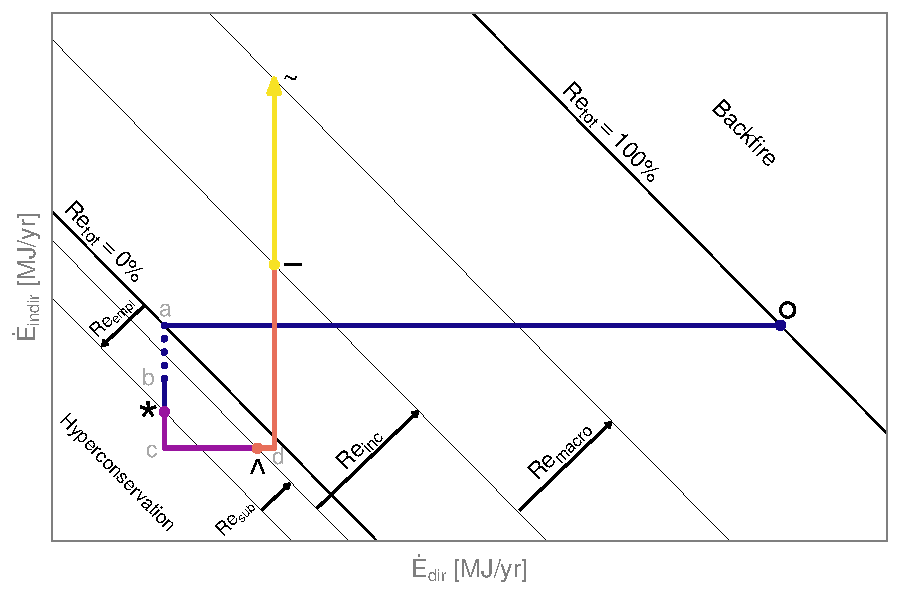
\includegraphics[width=\maxwidth]{figure/ExampleEnergyPathGraph-1} 

}

\caption{Notional energy plane. See Table~\ref{tab:path_graph_segments} for meanings of path segments.}\label{fig:ExampleEnergyPathGraph}
\end{figure}

\end{knitrout}

In the notional energy plane of Fig.~\ref{fig:ExampleEnergyPathGraph}, 
point $a$ lies on the $Re_{tot} = 0\%$ line
indicating that point $a$ (and the $Re_{tot} = 0\%$ line)
is the point from which all rebound effects 
($Re_{empl}$, $Re_{sub}$, $Re_{inc}$, and $Re_{\macro}$)
are measured.
If rebound effects cause 
total energy demand to return to the original energy consumption level 
(negative sloping line through the $\circ$ point), 
all expected energy savings are taken back by rebound effects. 
Thus, the line of constant energy consumption through the $\circ$ point is labeled
$Re_{tot} = 100\%$.
The contribution of each rebound effect to total rebound 
is represented by the distance that each component's segment
moves across the rebound isoquants.  
Total rebound ($Re_{tot}$) is measured linearly between and beyond the
$Re_{tot} = 0\%$ and $Re_{tot} = 100\%$ lines, 
with direct rebound in the $x$ direction and 
indirect rebound in the $y$ direction.
The region below and to the left of the $Re_{tot} = 0\%$ line
in Fig.~\ref{fig:ExampleEnergyPathGraph}
exhibits negative rebound, indicating hyperconservation.
The region above and to the right of the $Re_{tot} = 100\%$ line 
shows backfire, 
i.e., greater total energy consumption after the EEU than before it. 

In the notional energy plane (Fig.~\ref{fig:ExampleEnergyPathGraph}), 
emplacement rebound is negative ($Re_{empl} < 0$),
because the upgraded device has a lesser
embodied energy rate ($\rbempl{E}_{emb} > \raempl{E}_{emb}$,
as shown by point \emph{b} being below point \emph{a})
and has a lesser energy consumption rate for maintenance and disposal 
($\rbempl{E}_{\md} > \raempl{E}_{\md}$, 
as shown by point $*$ being below point \emph{b})
due to lower expenditure rates on these two categories
compared to the original device.

In Fig.~\ref{fig:ExampleCostPathGraph} segments \ab{} and \bstar{}
move in the negative $y$ direction,
consistent with the description above.
Segment \starc{} moves in the negative $y$ direction
by definition of the indirect substitution effect,
and segment \chat{} moves in the positive $x$ direction 
by the definition of the direct substitution effect. 
Both income effect segments (\hatd{} and \dbar{})
show more energy consumption, because net savings are spent
on goods and services that rely on at least some energy consumption.%
\footnote{
  We exclude the case of an inferior good, whose consumption decreases
  as real income increases, but 
  we note here the possibility of such behavior. 
  This behavior would
  however require a different utility model 
  besides the CES utility model,
  which we use throughout this analysis.
}
%
Segment \bartilde{} always moves in the positive $y$ direction,
because macro effects lead to additional indirect energy consumption.


%------------------------------
\subsubsection{The expenditure plane}
\label{sec:expenditure_path_graphs}
%------------------------------

A notional expenditure plane is shown in Fig.~\ref{fig:ExampleCostPathGraph}, 
with 
the direct expenditure rate on the energy service ($\rate{C}_{dir}$) on the $x$-axis and 
the indirect expenditure rate ($\rate{C}_{indir}$) on the $y$-axis.
Lines with negative slope through points $\circ$, $a$, $*$, and $\wedge$
indicate expenditure isoquants.
The line through the $\circ$ point is an isoquant for the
cost of purchasing the original consumption bundle
at the original prices.
The line through the $*$ point is an isoquant for the
cost of purchasing the original consumption bundle
at the new prices.


\begin{knitrout}
\definecolor{shadecolor}{rgb}{0.969, 0.969, 0.969}\color{fgcolor}\begin{figure}

{\centering 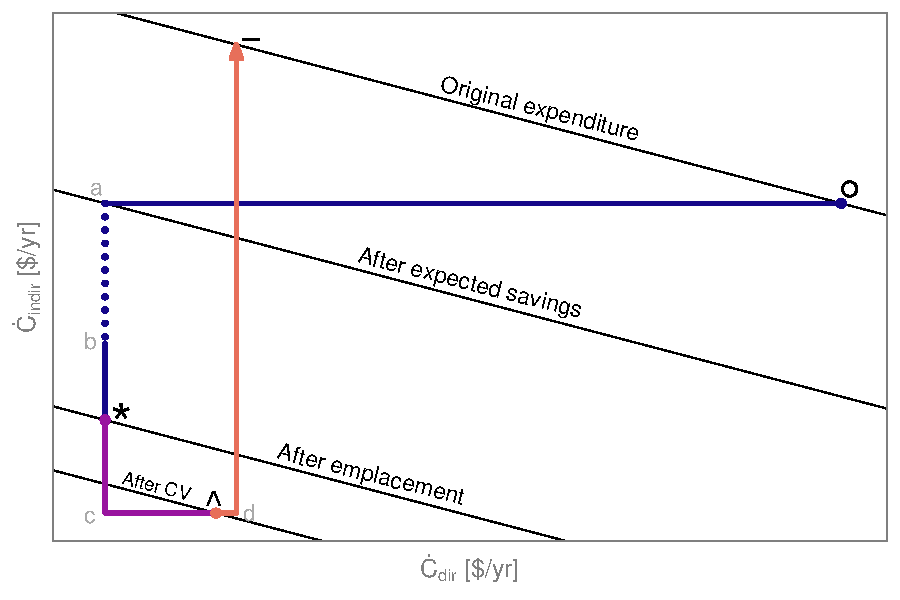
\includegraphics[width=\maxwidth]{figure/ExampleCostPathGraph-1} 

}

\caption{Notional expenditure plane. CV is compensating variation, the increase in consumption of the energy service and decrease in consumption of other goods and services to maintain constant utility. See Table~\ref{tab:path_graph_segments} for meanings of path segments.}\label{fig:ExampleCostPathGraph}
\end{figure}

\end{knitrout}

In the notional planes of
Figs.~\ref{fig:ExampleEnergyPathGraph} and~\ref{fig:ExampleCostPathGraph}, 
embodied energy rates and capital cost rates
(represented by segments \ab{} and \bstar{}) 
move in the same direction (both in the negative $y$ direction).
However, segments \ab{} and \bstar{} 
could both move in the positive $y$ direction, or
they could move in opposite directions, 
depending on the results of the independent analyses for 
embodied energy and capital cost rates.
The substitution effect along segments \starc{} and \chat{}
will together, by definition, lead to lower expenditure 
due to the energy service price decline and
the budget reducing compensating variation (CV). 
The income effect (segments \hatd{} and \dbar{}) must bring expenditure
back to the original expenditure line 
(equal to the budget constraint set by income in dollar or nominal terms) 
by assumptions about non-satiation and utility maximization 
in the device user's decision function.


%------------------------------
\subsubsection{The consumption plane}
\label{sec:consumption_path_graphs}
%------------------------------

A notional consumption plane is shown in Fig.~\ref{fig:ExampleConsPathGraph}.
The indexed rate of energy service consumption ($\rate{q}_s/\rbempl{q}_s$) is shown on the $x$-axis, and
the indexed rate of other goods consumption ($\rate{C}_o/\rbempl{C}_o$) is shown on the $y$-axis.
%Iso-expenditure loci of indexed energy service and other goods demand,
%are shown as lines with negative slope
Iso-expenditure loci of indexed energy service and other goods demand,
i.e. budget constraints,
are shown as lines with negative slope
(lines \circcirc{}, \starstar{}, \hathat{}, and \barbar{}). 
Note that budget constraints \circcirc{} and \barbar{} 
intersect at the $y$-axis,
because the prices of other goods and services don't change
as a result of the EEU.
(The $x$-axis of Fig.~\ref{fig:ExampleConsPathGraph} does not extend to $0$ at the left, 
so the intersection is not visible.)
Emplacement (by itself) does not alter consumption patterns, so
the rate of energy service consumption and 
the rate of other goods consumption are
unchanged across the emplacement effect
($\rbempl{q}_s = \raempl{q}_s$ and $\rbempl{C}_o = \raempl{C}_o$, respectively).
Thus, 
only movements after the $*$ point are visible as a path in the consumption plane, and
points $\circ$, \emph{a}, \emph{b}, and $*$ 
collapse to the same location in the consumption plane.

Indifference curves are denoted by \iicirc{} and \iibar{}
and represent lines of constant utility through the $\circ$ and $-$ points. 
Prior to the EEU, the consumption basket (of the energy service and other goods)
is represented by the $\circ$ point. 
The budget constraint,
here in real terms, i.e.,
the capacity to purchase either the energy service or other goods and services,
is shown as isoquant \circcirc{}.
The original budget constraint line (\circcirc{})
is tangent to the original indifference curve 
(\iicirc{}) at point $\circ$, the optimal consumption
bundle prior to the EEU.
The real budget line \starstar{}
indicates the (higher) capacity to purchase 
combinations of energy services and other goods and services
using the same money needed to purchase
the old consumption bundle but at the new, lower price
for the energy service,
thanks to the EEU.

The substitution effect leads to the cheaper, optimal
utility-preserving
consumption bundle at the $\wedge$ point. 
The substitution effect is shown by segments
\starc{} (the indirect component, which represents the decrease in other goods consumption) and
\chat{} (the direct component, which represents the increase in energy service consumption).
Although the substitution effect is calculated 
on the consumption plane, 
its impact 
can be seen in
the energy and expenditures planes 
(Figs.~\ref{fig:ExampleEnergyPathGraph}
and~\ref{fig:ExampleCostPathGraph}, respectively).

The income expansion path is a ray (\rr{}) from the origin through the $\wedge$ point
in the consumption plane.
In the consumption plane, the pre- and post-income-effect 
points ($\wedge$ and $-$, respectively)
lie along the \rr{} ray, due to homotheticity.
The increased consumption rate of the energy service is 
represented by segment \hatd{} 
in Figs.~\ref{fig:ExampleEnergyPathGraph}--\ref{fig:ExampleConsPathGraph}.
The increased consumption rate of other goods and services is 
represented by segments \dbar{} 
in Figs.~\ref{fig:ExampleEnergyPathGraph}--\ref{fig:ExampleConsPathGraph}.


\begin{knitrout}
\definecolor{shadecolor}{rgb}{0.969, 0.969, 0.969}\color{fgcolor}\begin{figure}

{\centering 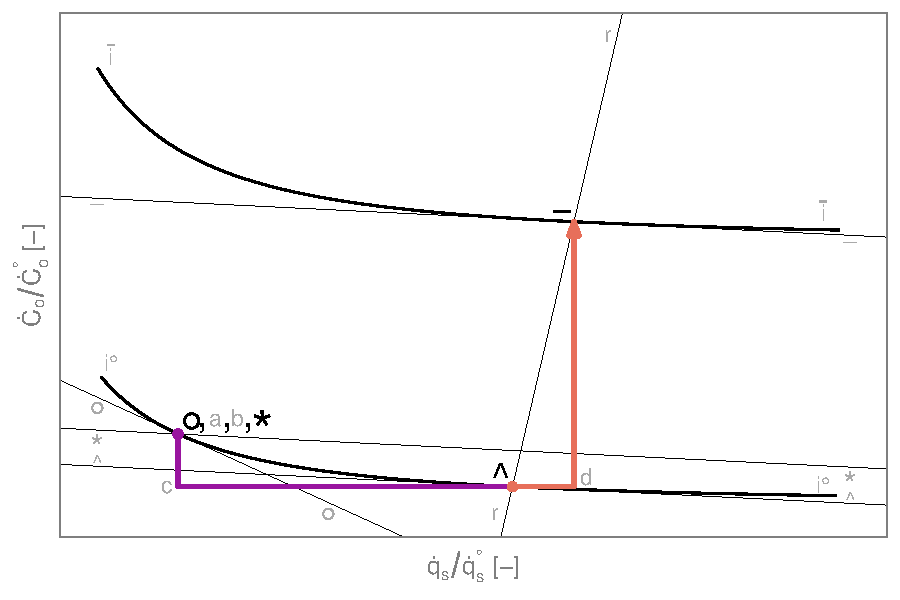
\includegraphics[width=\maxwidth]{figure/ExampleConsPathGraph-1} 

}

\caption{Notional consumption plane. See Table~\ref{tab:path_graph_segments} for meanings of path segments.}\label{fig:ExampleConsPathGraph}
\end{figure}

\end{knitrout}



%++++++++++++++++++++++++++++++
\subsection{Software tools}
\label{sec:software_tools}
%++++++++++++++++++++++++++++++

We developed an open source \texttt{R} package called \texttt{ReboundTools}
to standardize and distribute the methods for calculating rebound magnitudes in our framework.
\texttt{ReboundTools} can be found at \url{https://github.com/MatthewHeun/ReboundTools}.
(See \citet{Heun:2023aa}.)
\texttt{ReboundTools} provides functions for 
%
\begin{enumerate*}[label={(\roman*)}]
	
  \item reading input data from a spreadsheet,

  \item performing rebound calculations, and 
  
  \item generating rebound tables and rebound planes.
    
\end{enumerate*}
%
\texttt{ReboundTools} was used for 
all calculations and all rebound planes in this paper.

To find the path in storage to an example spreadsheet bundled with the package, 
users of \texttt{ReboundTools}
can call the function \texttt{ReboundTools::sample\_eeu\_data\_path()}.
After filling the example spreadsheet with parameters for an EEU, 
users can call two functions
(\texttt{ReboundTools::load\_eeu\_data()} and \texttt{ReboundTools::rebound\_analysis()})
to perform all rebound calculations described in this paper.
The function \texttt{ReboundTools::path\_graphs()} creates 
rebound paths in the energy, expenditure, and consumption planes.
Extensive documentation for \texttt{ReboundTools}
can be found at \url{https://matthewheun.github.io/ReboundTools/}.

In addition, an Excel workbook that performs identical rebound calculations 
using the framework of this paper
**** will be stored at the
Research Data Leeds Repository if this submission is accepted.  
The spreadsheet file is included with the submission of this paper. ****
% can be found at the data repository for this paper at
% \url{https://doi.org/10.5518/1201}.
(See \citet{Brockway:2023aa}.)


%%%%%%%%%%%%%%%%%%%%%%%%%%%%%%%%%%%%%%%%%%%%%%%%%%%%%%%%%%%%%%
\section{Results}
\label{sec:results}
%%%%%%%%%%%%%%%%%%%%%%%%%%%%%%%%%%%%%%%%%%%%%%%%%%%%%%%%%%%%%%

In this section we present rebound calculation results for two examples: 
energy efficiency upgrades of a car (Section~\ref{sec:car_example}) and 
an electric lamp (Section~\ref{sec:lamp_example}). 
Univariate sensitivity studies for both examples (car and lamp) 
can be found in Appendix~\ref{sec:sensitivity_analyses}.


%++++++++++++++++++++++++++++++
\subsection{Example 1: Purchase of a new car}
\label{sec:car_example}
%++++++++++++++++++++++++++++++

Armed with the parameter values from 
Tables~\ref{tab:car_parameters}--\ref{tab:car_elasticity_parameters}, 
and the equations in Section~\ref{PartI-sec:framework} of Part~I,
we calculate important values at each rebound stage,
as shown in Table~\ref{tab:car_stages_table}.
Note that Table~\ref{tab:car_stages_table} applies to the car user.
Across the macro effect (segment \bartilde{} in Fig.~\ref{fig:CarEnergyGraph}), 
changes occur only in the macroeconomy.
For the car user, no changes are recorded across the macro effect.
Thus, the $-$ (bar) and $\sim$ (tilde) columns
of Table~\ref{tab:car_stages_table} are identical.

% % latex table generated in R 4.3.2 by xtable 1.8-4 package
% % Wed Mar 13 08:36:10 2024
% \begin{table}[ht]
% \centering
% \caption{Results for car example with macro factor ($k$) assumed to be 1.} 
% \label{tab:car_stages_table}
% \begin{tabular}{rrrrrr}
%   \toprule
%   & $\circ$ (orig) & $*$ (star) & $\wedge$ (hat) & $-$ (bar) & $\sim$ (tilde) \\ 
%   \midrule
% $\eta$ [mile/gal] & 25.0 & 42.0 & 42.0 & 42.0 & 42.0 \\ 
%   $\eta$ [mile/MJ] & 0.197 & 0.332 & 0.332 & 0.332 & 0.332 \\ 
%   $p_s$ [\$/mile] & 0.105 & 0.063 & 0.063 & 0.063 & 0.063 \\ 
%   $\dot{q}_s$ [mile/yr] & 12,416 & 12,416 & 13,336 & 13,756 & 13,756 \\ 
%   $\dot{E}_s$ [MJ/yr] & 62,885 & 37,432 & 40,204 & 41,470 & 41,470 \\ 
%   $\dot{E}_{emb}$ [MJ/yr] & 2,429 & 2,857 & 2,857 & 2,857 & 2,857 \\ 
%   $\dot{C}_s$ [\$/yr] & 1,306 & 777 & 835 & 861 & 861 \\ 
%   $\dot{C}_{cap}$ [\$/yr] & 4,778 & 4,720 & 4,720 & 4,720 & 4,720 \\ 
%   $\dot{C}_{md}$ [\$/yr] & 2,731 & 2,710 & 2,710 & 2,710 & 2,710 \\ 
%   $\dot{C}_o$ [\$/yr] & 19,115 & 19,115 & 19,040 & 19,639 & 19,639 \\ 
%   $\dot{N}$ [\$/yr] & 0 & 608 & 626 & 0 & 0 \\ 
%   $\dot{M}$ [\$/yr] & 27,930 & 27,930 & 27,930 & 27,930 & 27,930 \\ 
%    \bottomrule
% \end{tabular}
% \end{table}

% latex table generated in R 4.3.2 by xtable 1.8-4 package
% Wed Mar 13 08:36:10 2024
\begin{table}[ht]
\centering
\caption{Results for car example with macro factor ($k$) assumed to be 1.} 
\label{tab:car_stages_table}
\begin{tabular}{rrrrr}
  \toprule
  & $\circ$ (orig) & $*$ (star) & $\wedge$ (hat) & $-$ (bar) \\ 
  \midrule
$\eta$ [mile/gal] & 25.0 & 42.0 & 42.0 & 42.0 \\ 
  $\eta$ [mile/MJ] & 0.197 & 0.332 & 0.332 & 0.332 \\ 
  $p_s$ [\$/mile] & 0.105 & 0.063 & 0.063 & 0.063  \\ 
  $\dot{q}_s$ [mile/yr] & 12,416 & 12,416 & 13,336 & 13,756 \\ 
  $\dot{E}_s$ [MJ/yr] & 62,885 & 37,432 & 40,204 & 41,470 \\ 
  $\dot{E}_{emb}$ [MJ/yr] & 2,429 & 2,857 & 2,857 & 2,857 \\ 
  $\dot{C}_s$ [\$/yr] & 1,306 & 777 & 835 & 861 \\ 
  $\dot{C}_{cap}$ [\$/yr] & 4,778 & 4,720 & 4,720 & 4,720 \\ 
  $\dot{C}_{md}$ [\$/yr] & 2,731 & 2,710 & 2,710 & 2,710 \\ 
  $\dot{C}_o$ [\$/yr] & 19,115 & 19,115 & 19,040 & 19,639 \\ 
  $\dot{N}$ [\$/yr] & 0 & 608 & 626 & 0 \\ 
  $\dot{M}$ [\$/yr] & 27,930 & 27,930 & 27,930 & 27,930 \\ 
   \bottomrule
\end{tabular}
\end{table}


Results are represented graphically on energy, expenditure, and consumption planes
in Figs.~\ref{fig:CarEnergyGraph}--\ref{fig:CarConsGraph}.
The energy plane (Fig.~\ref{fig:CarEnergyGraph})
shows the size of each rebound effect
for the car example.
Rebound components for the car upgrade are shown in Table~\ref{tab:car_results}.




\begin{knitrout}
\definecolor{shadecolor}{rgb}{0.969, 0.969, 0.969}\color{fgcolor}\begin{figure}

{\centering 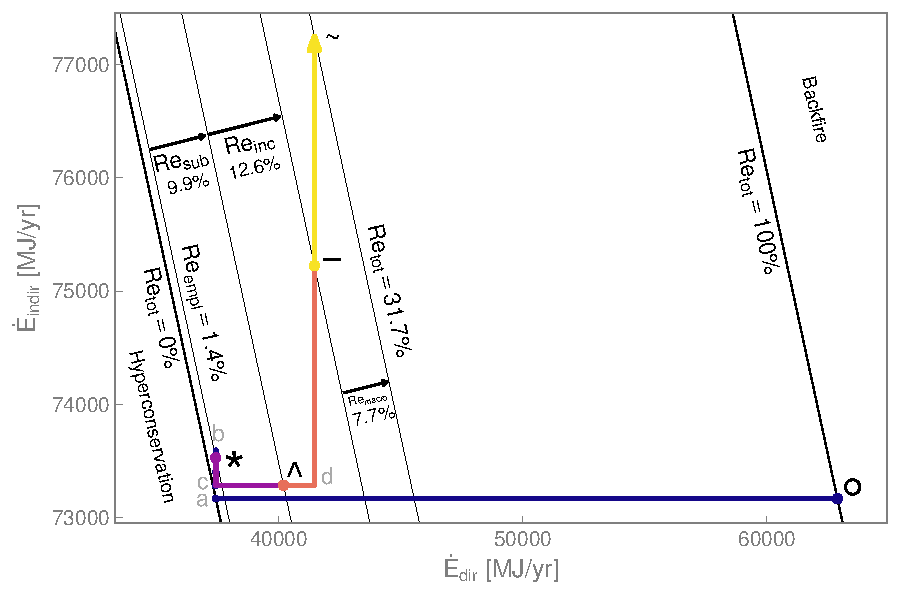
\includegraphics[width=\maxwidth]{figure/CarEnergyGraph-1} 

}

\caption{The energy plane for the car example. Macro factor ($k$) is assumed to be 1. See Table~\ref{tab:path_graph_segments} for meanings of path segments.}\label{fig:CarEnergyGraph}
\end{figure}

\end{knitrout}


\begin{knitrout}
\definecolor{shadecolor}{rgb}{0.969, 0.969, 0.969}\color{fgcolor}\begin{figure}

{\centering 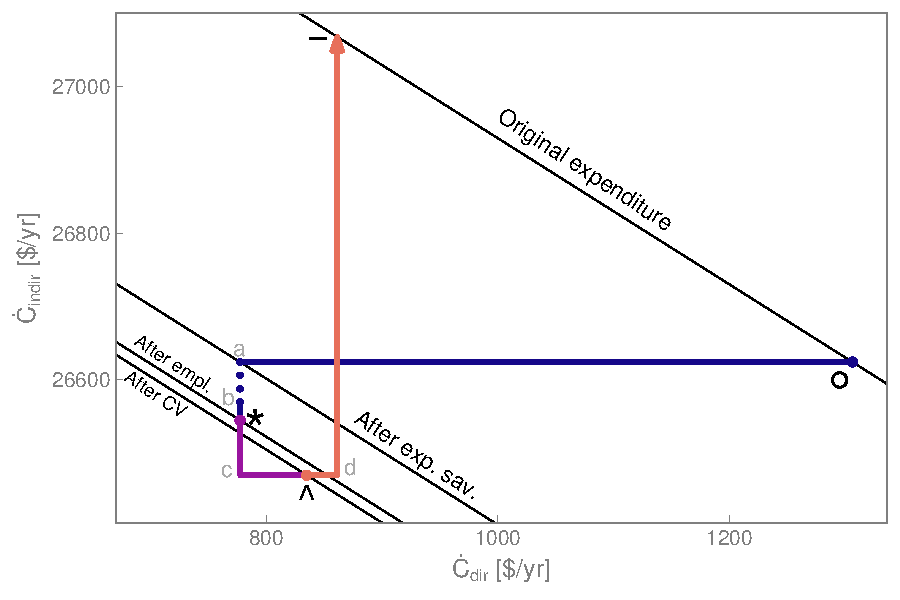
\includegraphics[width=\maxwidth]{figure/CarCostGraph-1} 

}

\caption{The expenditure plane for the car example. CV is compensating variation, the increase in consumption of the energy service and decrease in consumption of other goods and services to maintain constant utility. See Table~\ref{tab:path_graph_segments} for meanings of path segments.}\label{fig:CarCostGraph}
\end{figure}

\end{knitrout}


\begin{knitrout}
\definecolor{shadecolor}{rgb}{0.969, 0.969, 0.969}\color{fgcolor}\begin{figure}

{\centering 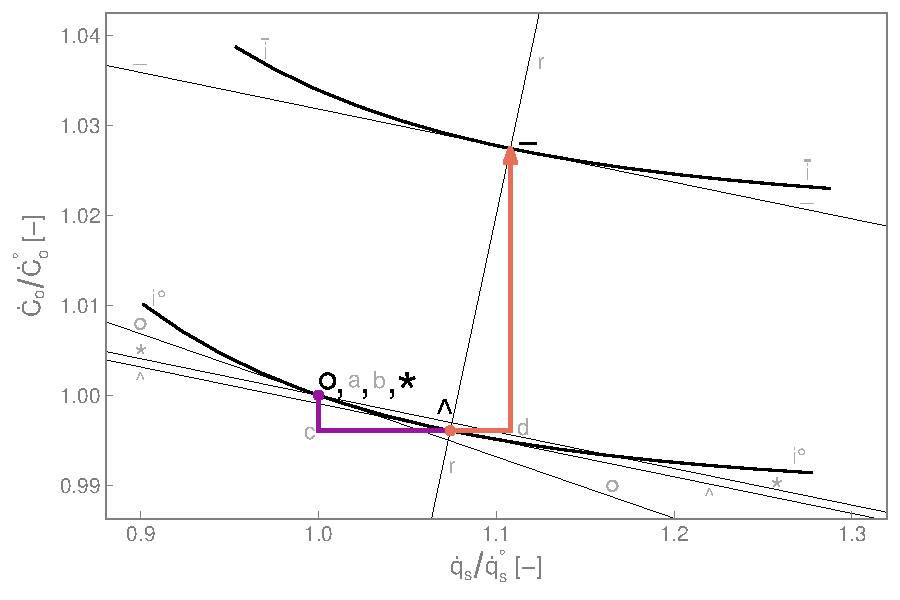
\includegraphics[width=\maxwidth]{figure/CarConsGraph-1} 

}

\caption{The consumption plane for the car example. See Table~\ref{tab:path_graph_segments} for meanings of path segments.}\label{fig:CarConsGraph}
\end{figure}

\end{knitrout}



% latex table generated in R 4.3.2 by xtable 1.8-4 package
% Wed Mar 13 08:36:11 2024
\begin{table}[ht]
\centering
\caption{Car example: rebound results with macro factor ($k$) assumed to be 1.} 
\label{tab:car_results}
\begingroup\footnotesize
\begin{tabular}{rr}
  \toprule
Rebound term & Value [\%] \\ 
  \midrule
$Re_{dempl}$ & 0.0 \\ 
  $Re_{emb}$ & 1.7 \\ 
  $Re_{md}$ & $-$0.3 \\ 
  $Re_{dsub}$ & 10.9 \\ 
  $Re_{isub}$ & $-$1.0 \\ 
  $Re_{dinc}$ & 5.0 \\ 
  $Re_{iinc}$ & 7.6 \\ 
  $Re_{macro}$ & 7.7 \\ 
   \midrule
$Re_{tot}$ & 31.7 \\ 
   \bottomrule
\end{tabular}
\endgroup
\end{table}



The \empleffect{} has three components:
the direct emplacement effect, 
the embodied energy effect, and 
the maintenance and disposal effect.
Rebound from the direct emplacement effect 
($Re_{dempl}$) is 0.0\% always, 
because energy takeback (and, therefore, rebound)
occurs after the upgraded device is emplaced.
Indirect rebound due to the embodied energy effect
($Re_{emb}$) is 1.7\%,  
due to the higher embodied energy rate
($\Delta \raempl{E}_{emb} = 429$~MJ/yr)
stemming from the electric battery in the hybrid EV car.
Rebound due to the maintenance and disposal effect
($Re_{\md}$) is small and negative
($-0.3$\%),
because of the slightly lower maintenance and disposal costs
for the hybrid EV car.

The \subeffect{} has two components:
direct and indirect substitution effect rebound.
Rebound from direct substitution ($Re_{dsub}$) is 
positive, as expected (10.9\%). 
The car user will, on average, prefer more driving purely 
from the change in relative prices because of the fuel economy enhancements
(42~mpg $>$ 25~mpg).
In other words, 
due the relative price change,
the more fuel-efficient car is driven 7.4\% further
each year. 
Conversely, the indirect substitution effect ($Re_{isub}$)
is slightly negative ($-1.0$\%)
to achieve the same level of utility after increased driving. 
Indeed, across the substitution effect,
less money is spent on other goods
($\Delta \rasub{C}_o = -75.18$~\$/yr).
In Appendix~\ref{sec:price_elasticities_sensitivity} we show how the
displacement along an indifference curve alters the price elasticities,
and in particular, that the uncompensated own price elasticity declines
in magnitude. The decline slows the rate of additional consumption of
energy intensive driving, and attenuates the microeconomic rebound
relative to assuming constant price elasticities.

The \inceffect{} also has two components:
direct and indirect income effect rebound.
The direct income effect
($Re_{dinc}$) is positive
(5.0\%), 
because the car user allocates some
net savings to additional driving. 
Rebound from the indirect income effect 
($Re_{iinc}$) is positive (7.6\%)
due to higher spending on other goods. 
Thus, the net savings after the substitution effect
($\rasub{N} = 625.79$~\$/yr) 
translates into positive direct and indirect income
rebound at the microeconomic level. 
Total microeconomic rebound (emplacement, substitution, and income effects)
sums to $Re_{micro} = 24.0$\%.

Finally, in Part~I we noted that 
the link between macroeconomic and microeconomic rebound 
is largely unexplored, 
so we assume a value of $k = 1$ for both examples, initially.
We return to the matter of calibrating $k$
in the Discussion (Section~\ref{sec:calibrating_k}).
With $k$ assumed to be 1,
the \macroeffect{} leads to macroeconomic rebound
($Re_{\macro}$) of 7.7\% 
for the car example,
due to economic expansion caused by 
productivity enhancements arising from the more-efficient provision of the 
energy service (transportation).


%++++++++++++++++++++++++++++++
\subsection{Example 2: Purchase of a new electric lamp}
\label{sec:lamp_example}
%++++++++++++++++++++++++++++++

With the parameter values from 
Tables~\ref{tab:lamp_parameters}--\ref{tab:lamp_elasticity_parameters} 
and the equations in Section~\ref{PartI-sec:framework} of Part~I in hand,
we calculate important values at each rebound stage,
as shown in Table~\ref{tab:lamp_stages_table}.
Similar to Table~\ref{tab:car_stages_table}, 
Table~\ref{tab:lamp_stages_table} applies to the lamp user, 
so no changes are recorded across the macro effect, and
the $-$ (bar) and $\sim$ (tilde) columns
of Table~\ref{tab:lamp_stages_table} are identical.

% latex table generated in R 4.3.2 by xtable 1.8-4 package
% Wed Mar 13 08:36:11 2024
\begin{table}[ht]
\centering
\caption{Results for lamp example with macro factor ($k$) assumed to be 1.} 
\label{tab:lamp_stages_table}
\begin{tabular}{rrrrr}
  \toprule
  & $\circ$ (orig) & $*$ (star) & $\wedge$ (hat) & $-$ (bar) \\ 
  \midrule
$\eta$ [\lmhr/\kWhr] & 8,833 & 81,800 & 81,800 & 81,800 \\ 
  $\eta$ [\lmhr/MJ] & 2,454 & 22,722 & 22,722 & 22,722 \\ 
  $p_s$ [\$/\lmhr] & 0.00001457 & 0.00000157 & 0.00000157 & 0.00000157 \\ 
  $\dot{q}_s$ [\lmhr/yr] & 580,350 & 580,350 & 1,412,867 & 1,413,439 \\ 
  $\dot{E}_s$ [MJ/yr] & 236.5 & 25.5 & 62.2 & 62.2 \\ 
  $\dot{E}_{emb}$ [MJ/yr] & 1.222 & 0.650 & 0.650 & 0.650 \\ 
  $\dot{C}_s$ [\$/yr] & 8.46 & 0.91 & 2.22 & 2.22 \\ 
  $\dot{C}_{cap}$ [\$/yr] & 1.04 & 0.12 & 0.12 & 0.12 \\ 
  $\dot{C}_{md}$ [\$/yr] & 0.00 & 0.00 & 0.00 & 0.00 \\ 
  $\dot{C}_o$ [\$/yr] & 27,920 & 27,920 & 27,916 & 27,927 \\ 
  $\dot{N}$ [\$/yr] & 0.00 & 8.47 & 11.31 & 0.00 \\ 
  $\dot{M}$ [\$/yr] & 27,930 & 27,930 & 27,930 & 27,930 \\ 
   \bottomrule
\end{tabular}
\end{table}






Results are represented graphically on energy, expenditure, and consumption planes
in Figs.~\ref{fig:LampEnergyGraph}--\ref{fig:LampConsGraph}.
The energy plane (Fig.~\ref{fig:LampEnergyGraph})
shows the size of each rebound effect
for the lamp example.
Rebound components for the lamp upgrade are shown in Table~\ref{tab:lamp_results}.

The \empleffect{} rebound components start with
the direct emplacement effect ($Re_{dempl}$),
which is always $0.0$\%.
Indirect rebound due to the embodied energy effect
($Re_{emb}$) is $-0.3$\%.
Although the LED lamp has higher embodied energy 
($\aempl{E}_{emb} = 6.50$~MJ)
than the incandescent lamp 
($\bempl{E}_{emb} = 2.20$~MJ),
the LED lamp has a much longer lifetime,
meaning that the LED embodied energy \emph{rate}
($\raempl{E}_{emb} = 0.65$~MJ/yr)
is less than the incandescent embodied energy rate
($\rbempl{E}_{emb} = 1.22$~MJ/yr).
Thus, the change in embodied energy rate ($\Delta \raempl{E}_{emb}$)
is $-0.57$~MJ/yr, 
and embodied energy rebound is negative
($Re_{emb} = -0.3$\%).
Rebound due to the maintenance and disposal effect
($Re_{\md}$) is 0.0\%,
because we assume no difference in maintenance and disposal costs between 
the incandescent lamp and the LED lamp.%
\footnote{
  Maintenance cost rates for both incandescent and LED lamps are likely to be equal 
  and negligible;
  lamps are usually installed and forgotten.
  Real-world disposal cost differences between the incandescent and LED technologies
  are also likely to be negligible. 
  However, if ``disposal'' includes recycling processes, 
  cost rates may be different between the two technologies
  due to the wide variety of materials in LED lamps compared to incandescent lamps.
}

Direct \subeffect{} rebound 
($Re_{dsub}$) is 17.4\%
due to the much higher LED lamp efficiency
($\amacro{\eta} = 81.8$~lm/W) 
compared to the incandescent lamp
($\bempl{\eta} = 8.83$~lm/W),
leading to increased demand for lighting
(from $\rbsub{q}_s = 580,350$~\lmhr/yr
to $\rasub{q}_s = 1,412,867$~\lmhr/yr)
as shown by segment \chat{} in Fig.~\ref{fig:LampConsGraph}.
To maintain constant utility, 
consumption of other goods is reduced
($\Delta \rasub{C}_o = -4.15$~\$/yr), 
as shown by segment \starc{} in Fig.~\ref{fig:LampConsGraph},
yielding indirect substitution effect rebound
($Re_{isub}$) of $-6.4$\%.

\Inceffect{} rebound arises from spending net energy cost savings
associated with converting from the incandescent lamp to the LED lamp
($\rbinc{N} = 11.31$~\$/yr).
Direct income effect rebound 
($Re_{dinc}$) is 0.01\%,
positive but small, 
as the lamp user allocates
some of the net savings to additional demand for lighting.
The indirect income effect rebound is large
($Re_{iinc} = 17.4$\%),
due to the energy implications of increased spending on other goods.
Total microeconomic level rebound (emplacement, substitution, and income effects)
sums to $Re_{micro} = 28.1$\%.

Finally, \macroeffect{} rebound
($Re_{\macro}$) is 13.0\%
with $k$ assumed to be 1,
due to economic expansion caused by 
productivity enhancements arising from the more-efficient provision of the 
energy service (lighting).


\begin{knitrout}
\definecolor{shadecolor}{rgb}{0.969, 0.969, 0.969}\color{fgcolor}\begin{figure}

{\centering 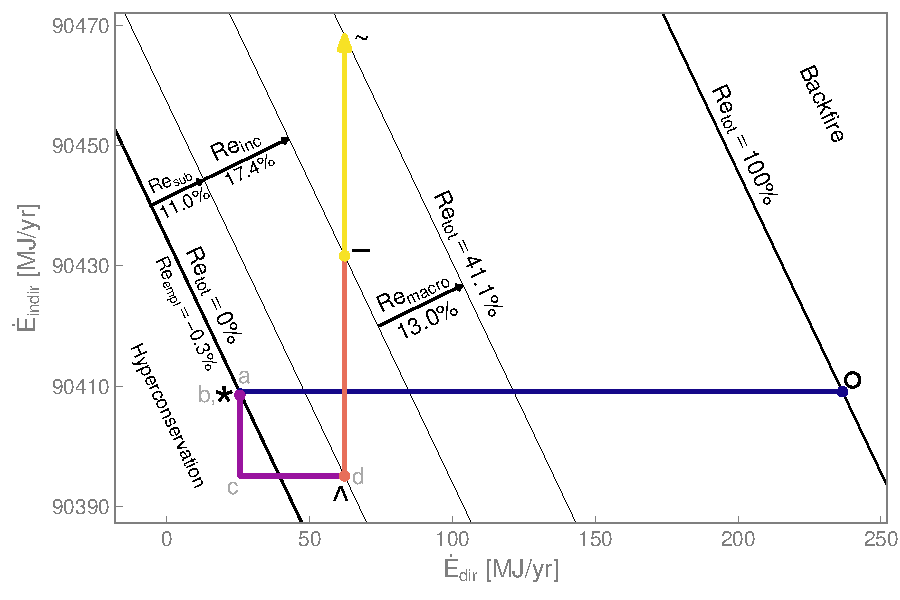
\includegraphics[width=\maxwidth]{figure/LampEnergyGraph-1} 

}

\caption{The energy plane for the lamp example. Macro factor ($k$) is assumed to be 1. See Table~\ref{tab:path_graph_segments} for meanings of path segments.}\label{fig:LampEnergyGraph}
\end{figure}

\end{knitrout}


\begin{knitrout}
\definecolor{shadecolor}{rgb}{0.969, 0.969, 0.969}\color{fgcolor}\begin{figure}

{\centering 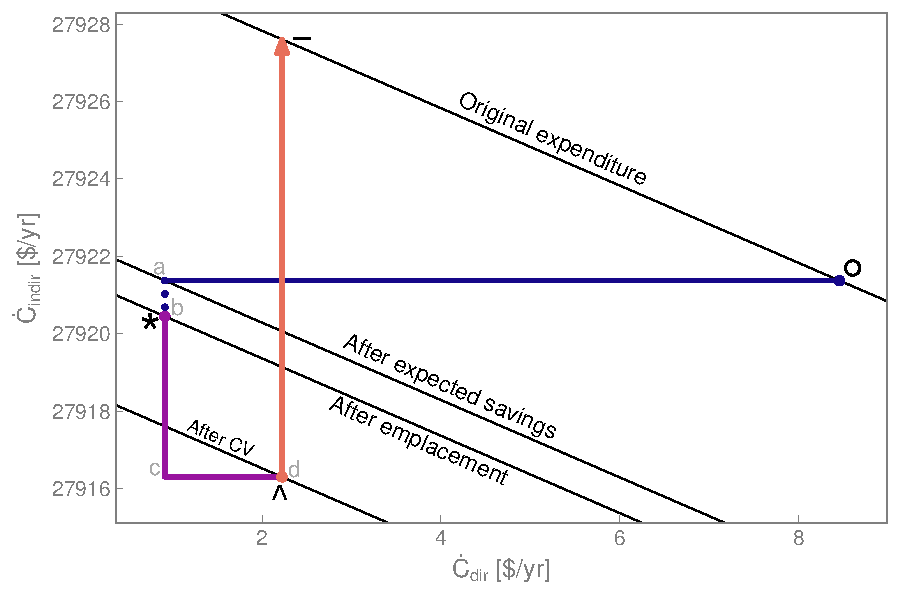
\includegraphics[width=\maxwidth]{figure/LampCostGraph-1} 

}

\caption{Expenditure plane for the lamp example. CV is compensating variation, the increase in consumption of the energy service and decrease in consumption of other goods and services to maintain constant utility. See Table~\ref{tab:path_graph_segments} for meanings of path segments.}\label{fig:LampCostGraph}
\end{figure}

\end{knitrout}


\begin{knitrout}
\definecolor{shadecolor}{rgb}{0.969, 0.969, 0.969}\color{fgcolor}\begin{figure}

{\centering 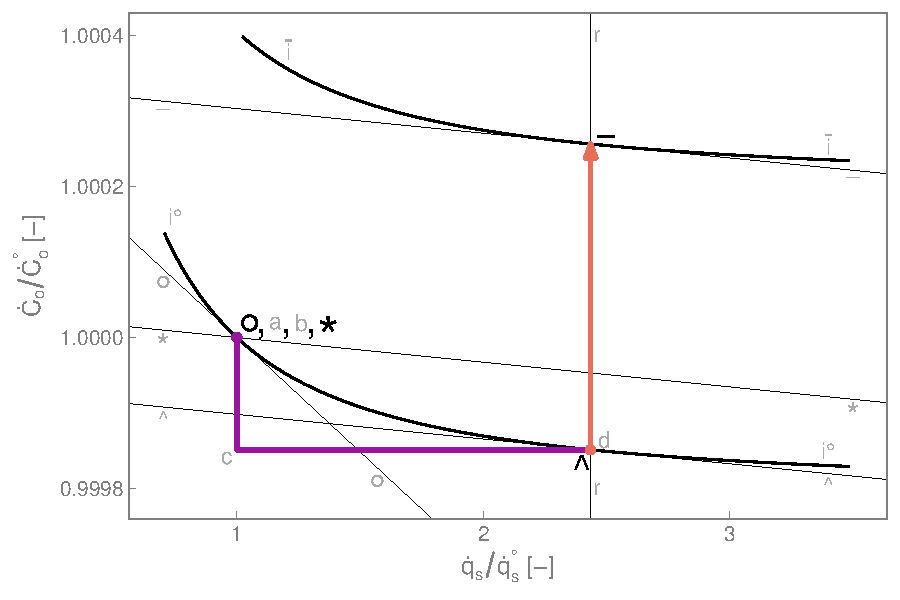
\includegraphics[width=\maxwidth]{figure/LampConsGraph-1} 

}

\caption{Consumption plane for the lamp example. See Table~\ref{tab:path_graph_segments} for meanings of path segments.}\label{fig:LampConsGraph}
\end{figure}

\end{knitrout}


% latex table generated in R 4.3.2 by xtable 1.8-4 package
% Wed Mar 13 08:36:13 2024
\begin{table}[ht]
\centering
\caption{Lamp example: rebound results with macro factor ($k$) assumed to be 1.} 
\label{tab:lamp_results}
\begin{tabular}{rr}
  \toprule
Rebound term & Value [\%] \\ 
  \midrule
$Re_{dempl}$ & 0.0 \\ 
  $Re_{emb}$ & $-$0.3 \\ 
  $Re_{md}$ & 0.0 \\ 
  $Re_{dsub}$ & 17.4 \\ 
  $Re_{isub}$ & $-$6.4 \\ 
  $Re_{dinc}$ & 0.0 \\ 
  $Re_{iinc}$ & 17.4 \\ 
  $Re_{macro}$ & 13.0 \\ 
   \midrule
$Re_{tot}$ & 41.1 \\ 
   \bottomrule
\end{tabular}
\end{table}



%%%%%%%%%%%%%%%%%%%%%%%%%%%%%%%%%%%%%%%%%%%%%%%%%%%%%%%%%%%%%%
\section{Discussion}
\label{sec:discussion}
%%%%%%%%%%%%%%%%%%%%%%%%%%%%%%%%%%%%%%%%%%%%%%%%%%%%%%%%%%%%%%



\begin{table}
\footnotesize
\centering
\caption{Comparison of substitution
         income effects
         ($Re_{dinc}$, $Re_{iinc}$, and $Re_{inc}$) and
         total ($Re_{tot}$) rebound
         between
         the CES utility model and satiated
         consumption of the energy service for the
         car and lamp examples.}
\label{tab:utility_model_comparison}
\begin{tabular}{r r r r r r r}
\toprule
                 & \multicolumn{3}{c}{Car example}
                                                & \multicolumn{3}{c}{Lamp example} \\
Rebound term     & CES & Satiated & CPE         & CES & Satiated & CPE             \\
\midrule
$Re_{dsub}$ [\%] &     &          &             &     &          &                 \\
$Re_{isub}$ [\%] &     &          &             &     &          &                 \\
\midrule
$Re_{sub}$ [\%]  &     &          &             &     &          &                 \\
\midrule
$Re_{dinc}$ [\%] & 
                       & 
                                  &
                                                & 
                                                      & 
                                                                 &               \\
$Re_{iinc}$ [\%] & 
                       & 
                                  &
                                                & 
                                                      & 
                                                                 &                \\
\midrule
$Re_{inc}$ [\%] & 
                       & 
                                  &
                                                & 
                                                      & 
                                                                 &                \\
\midrule
$Re_{tot}$ [\%] & 
                       & 
                                  &
                                                & 
                                                      & 
                                                                 &                \\
\bottomrule
\end{tabular}
\end{table}



%++++++++++++++++++++++++++++++
\subsection{A first attempt at calibrating $k$}
\label{sec:calibrating_k}
%++++++++++++++++++++++++++++++



Few previous studies explored link 
between microeconomic and macroeconomic rebound.
Inspired by \citet{Borenstein:2015aa} and others, 
the framework developed in Section~\ref{PartI-sec:framework} of Part~I
links macroeconomic rebound to microeconomic rebound 
via the macro factor~($k$) that scales
magnitudes in the microeconomic portion of the framework. 
(See Section~\ref{PartI-sec:macro_effect_main_paper} of Part~I.)

For the results presented in Section~\ref{sec:results} above, 
we assumed a placeholder value of $k = 1$,
meaning that every \$1 of spending by the device user in the income effect
generates only \$1 of additional economic activity in the broader economy.
In combination, the framework presented in Section~\ref{PartI-sec:framework} of Part~I, 
the results obtained in Section~\ref{sec:results} of this paper, and
recent calculations of total rebound in general equilibrium frameworks allow, 
for the first time, 
a discussion about calibrating $k$.
After calibrating $k$, 
macro rebound and total rebound can be calculated.

To calibrate the macro factor ($k$),
we treat macro rebound ($Re_{\macro}$) as a residual.
The macro factor ($k$) becomes an unknown parameter whose value is to be chosen
such that $Re_{\macro}$
is sufficient to achieve an expected value for total rebound ($Re_{tot}$).%
\footnote{
  This approach means that the calibrated value of $k$ incorporates all 
  macroeconomic rebound sub-effects included in the studies
  whose total rebound value we calibrate against.
}
%
We take the expected value for $Re_{tot}$ from 
\citet{Brockway:2021ww}.
Four of 33 studies reviewed by \citet{Brockway:2021ww}
examined total rebound from only consumer EEUs in a computable general
equilibrium (CGE) framework. 
The average total rebound ($Re_{tot}$) 
for the four consumer studies is 54\%.%
\footnote{
  The average total rebound among all 33 studies stood at 63\%,
  supporting the claim by \citet{Turner:2013aa} that consumer
  and producer rebounds vary.
}
%
The calibrated values of $k$ that give identical 
$Re_{tot} = 54$\% 
for both examples are
$k = 3.9$
for the car example and
$k = 2.0$ 
for the lamp example.

Qualitative differences in benefits from EEUs as well as the considerable 
variance in $Re_{tot}$ in 33 surveyed studies~\citep{Brockway:2021ww}
indicates that total rebound from one EEU is likely to be different from 
total rebound from another EEU. 
For a first approximation of a calibration for $k$,
we take $k \approx 3$,
being between the values of $k$ 
calculated from the car and lamp examples.
Note that $k \approx 3$ implies that 
every \$1 of net savings spent by the device user ($\raempl{N}$)
generates \$3 of additional economic 
activity in the broader economy.
We multiply $k \raempl{N}$ by the energy intensity of the economy ($I_E$) to 
find the energy implications of macro-effect respending throughout the economy.

There are three ways to interpret $k \approx 3$.
First, $k \approx 3$ can be considered the average long-run 
economic growth generated
by the productivity increase implied by the EEU and subsequent
productivity increases benefitting from the EEU.
Efficiency increases in equipment drive a significant part of 
long-run productivity growth \citep{Greenwood1997}, therefore a large
long-run effect is plausible,
even if the initial productivity
change occurred in household production which is not accounted in GDP.
(See Section~\ref{PartI-sec:macro_effect_main_paper} of Part~I 
for further discussion of this point.)
Second, it could be that growth is less than 
\$3 for every \$1 of respending,
but that the macroeconomic ``energy price effect'' (a decline in 
energy prices due to the fallen demand) induces consumption at a higher
energy intensity than that of the pre-EEU economy. 
Third, from the demand-side perspective
entertained by \citet{Borenstein:2015aa}, 
$k \approx 3$ could be interpreted as 
growth induced by the device user's spending of net savings with
a marginal propensity to consume (MPC)
of approximately $0.75$ that translates into a multiplier of 3. 
(See Fig.~\ref{PartI-fig:k_vs_mpc} 
in Appendix~\ref{PartI-sec:income_macro_mpc} of Part~I.)
$\MPC \approx 0.75$ is a reasonable value, 
being in the upper half of recent estimates from \citet{Carroll2017}.
Although the cause of the growth in economic activity and energy consumption from an EEU 
is a supply-side productivity shock,
the subsequent demand-side effects may well be interpreted as a multiplier effect, 
caused by higher real income instead of by higher monetary income.

After calibrating $k \approx 3$, 
we can recalculate all rebound components in our framework.
Emplacement ($Re_{empl}$), substitution ($Re_{sub}$), and income ($Re_{inc}$) rebound
magnitudes are unchanged after calibrating $k \approx 3$.
However, we see that choosing a placeholder value of $k = 1$
resulted in a low value for $Re_{\macro}$ and, therefore, $Re_{tot}$
in Section~\ref{sec:results}.
In Figs.~\ref{fig:CarEnergyGraph} and~\ref{fig:LampEnergyGraph},
the macro effect segments (\bartilde{})
should be three times longer than they appear.
In Tables~\ref{tab:car_results} and~\ref{tab:lamp_results},
the values of macro rebound ($Re_{\macro}$) should triple to
23.2\% and
39.0\%, and
the values of total rebound ($Re_{tot}$) should increase to 
47.2\% and
67.1\%
for the car and lamp examples,
respectively.
For the remainder of this paper, 
we use the calibrated value of $k \approx 3$.


%++++++++++++++++++++++++++++++
\subsection{Comparison between the car and lamp case studies}
\label{sec:case_study_comparison}
%++++++++++++++++++++++++++++++



Tables~\ref{tab:car_results} and~\ref{tab:lamp_results}
and our calibration of $k \approx 3$ in Section~\ref{sec:calibrating_k} 
enable fuller comparisons between the car and lamp examples. 
Several points can be made.

First, 
the magnitude of every rebound effect is different between the two examples, 
the exception being direct emplacement rebound ($Re_{dempl}$)
which is always 0.0 by definition.
The implication is that every EEU needs to be analyzed separately. 
Values for rebound effects  
for one EEU should never be assumed to apply to a different EEU.

Second, 
one cannot know \emph{a-priori} which rebound effects
will be large and which will be small
for a given EEU.
Furthermore, some rebound effects are dependent upon economic parameters,
such as energy intensity ($I_E$).
Thus, it is important to calculate the magnitude of all rebound effects 
for each EEU in each economy.

Third,
the two examples illustrate the fact that 
embodied energy rebound ($Re_{emb}$) can be positive or negative,
as discussed in Section~\ref{PartI-sec:empl_effect_main_paper} of Part~I.
The car's embodied energy rebound is positive ($1.7$\%) 
because of the high embodied energy of the EV's battery
relative to the internal combustion engine vehicle. 
Although the LED lamp's embodied energy is larger than the 
incandescent lamp's embodied energy, 
the LED lamp's embodied energy rebound is negative ($-0.3$\%),
due to the longer life of the LED lamp compared to the incandescent lamp.
Thus, each EEU should be analyzed independently for its embodied energy rebound.

Fourth,
macro effect rebound is different between the two examples, 
owing to differences in net income ($\raempl{N}$) relative to expected savings ($\Sdot$).
(For the car, $Re_{macro}$ is $23.2$\%.
For the lamp, $Re_{macro}$ is $39.0$\%.)
The efficiency gain for the lamp is far greater than the efficiency gain for the car,
leading to much different rates of net income ($\raempl{N}$) and
different macro rebound values.

% I think there is really no claim in this.
% Fifth,
% in both examples the macro effect rebound ($Re_{macro}$) is much larger than
% any single micro rebound component. 
% However, the sum of micro rebound components 
% ($Re_{micro} = Re_{empl} + Re_{sub} + Re_{inc}$) 
% is close in magnitude to the macro rebound ($Re_{macro}$).
% These observations are likely to be the result of 
% $Re_{macro}$ being the sum of several macroeconomic sub-effects,
% among which we don't discriminate in this framework.
% (See Table~\ref{PartI-tab:rebound_typology} in Part~I
% for a list of macro rebound effects.)


%++++++++++++++++++++++++++++++
\subsection{Comparison to previous rebound estimates} 
\label{sec:comparison_to_other_rebound_estimates}
%++++++++++++++++++++++++++++++

Tables~\ref{tab:rebound_car_comparisons} and~\ref{tab:rebound_lamp_comparisons}
compare car and lamp results (with $k \approx 3$) to 
results from previous studies.
% For punctuation of "rather" here, see https://linguaholic.com/linguablog/comma-before-rather/.
The comparison studies are neither comprehensive nor
definitive of car and lamp EEUs; 
rather, they are examples that show the sort of calculations and estimations
carried out in the general literature using a variety of methods. 
That said, many of the studies are highly cited,
thereby carrying sufficient academic weight for our purposes.
Tables~\ref{tab:rebound_car_comparisons} and~\ref{tab:rebound_lamp_comparisons}
and their associated references 
enable two types of observations, comparing
%
\begin{enumerate*}[label={(\roman*)}]
	
  \item coverage of rebound components and
  
  \item magnitudes and associated calculation or estimation methods.
    
\end{enumerate*}


% The next command tells RStudio to do "Compile PDF" on HSB_results.Rnw,
% instead of this file, thereby eliminating the need to switch back to HSB_results.Rnw 
% before building the paper.
%!TEX root = ../HSB_results.Rnw


\begin{landscape}
\begin{table}
\footnotesize
\begin{center}
\caption{Rebound magnitude comparisons for the car example. All numbers in \%.
         Note that 
         $Re_{tot} = Re_{empl} + Re_{sub} + Re_{inc} + Re_{macro}$, 
         $Re_{tot} = Re_{micro} + Re_{macro}$, and 
         $Re_{tot} = Re_{dir} + Re_{indir}$.}
\label{tab:rebound_car_comparisons}
\begin{tabular}{ c l l l c c c c @{\hspace*{10mm}} c c @{\hspace*{10mm}} c }
\toprule
  &               &          &                 & \multicolumn{3}{c}{$Re_{micro}$}      & $Re_{macro}$ & $Re_{dir}$ & $Re_{indir}$ & $Re_{tot}$ \\ 
  & Rebound study & Coverage & Analysis method & $Re_{empl}$ & $Re_{sub}$ & $Re_{inc}$ &              &            &              &            \\ 
\midrule
 & This paper & U.S., & Energy, expenditure, and  & $1.4$
                                                  & $9.9$
                                                  & $12.6$
                                                  & $23.2$
                                                  & $15.9$
                                                  & $31.3$
                                                  & $47.2$  \\
 & (2023)     & 2020  & consumption planes        & & & & & & &   \\
\midrule
1 & \citeauthor{Small:2007aa}  & U.S.,      & Elasticity of VMT w.r.t.\ & & & & & 4.5 (short run, &  &  \\
  & \citeyearpar{Small:2007aa} & 1967--2001 & fuel cost per mile        & & & & & 1967--2001)     &  &  \\
  &                            &            &                           & & & & & 22.2 (long run, &  &  \\
  &                            &            &                           & & & & & 1967--2001)     &  &  \\
  &                            &            &                           & & & & & 2.2 (short run, &  &  \\
  &                            &            &                           & & & & & 1997--2001)     &  &  \\
  &                            &            &                           & & & & & 10.7 (long run, &  &  \\
  &                            &            &                           & & & & & 1997--2001)     &  &  \\
\midrule
2 & \citeauthor{Greene2012}  & U.S.,      & Elasticities of transport   & & & & &  4 (short run) & & \\
  & \citeyearpar{Greene2012} & 1966--2007 & fuel w.r.t.\ price \&       & & & & & 16 (long run)  & & \\
  &                          &            & efficiency                  & & & & &                & & \\
\midrule
3 & \citeauthor{Koesler:2013aa}  & Germany, & Static CGE model,        & & & & & $\le$ 64 & $\le$ 16 & 56  \\
  & \citeyearpar{Koesler:2013aa} & 2009     & 10\% efficiency shock    & & & & &          &          &     \\
\midrule
4 & \citeauthor{Thomas:2013ab}  & U.S., & Expenditure/cross price   & & & & & 10 & 6 &  \\
  & \citeyearpar{Thomas:2013ab} & 2004  & elasticities of personal  & & & & &    &   &  \\
  &                             &       & transport fuels, using    & & & & &    &   &  \\
  &                             &       & household spending        & & & & &    &   &  \\
  &                             &       & survey data               & & & & &    &   &  \\
\midrule
5 & \citeauthor{Borenstein:2015aa}  & U.S., & Microeconomic &  & 13      & 11 & & & &  \\
  & \citeyearpar{Borenstein:2015aa} & 2012  & framework     &  & (6--28) &    & & & &  \\
\midrule
6 & \citeauthor{Chitnis:2015}  & UK,                       & Estimated own/cross price  & & 72 & 5 & & 55 & 23 & 86 \\
  & \citeyearpar{Chitnis:2015} & 1964--2014                & elasticities of transport  & &    &   & &    &    &    \\
  &                            &                           & fuels, uses household      & &    &   & &    &    &    \\
  &                            &                           & spending survey data       & &    &   & &    &    &    \\
\midrule
7 & \citeauthor{Gillingham:2015aa}  & Pennsylvania, & Estimation of gasoline      & & & & & 10 (short run) & &  \\
  & \citeyearpar{Gillingham:2015aa} & 2000--2010    & price elasticity of driving & & & & &                & &  \\
  &                                 &               & demand, from dataset        & & & & &                & &  \\
  &                                 &               & of 75 million vehicle       & & & & &                & &  \\
  &                                 &               & inspection records,         & & & & &                & &  \\
  &                                 &               & including odometer data     & & & & &                & &  \\
\midrule
8 & \citeauthor{Stapleton:2016}  & UK         & Elasticity of VMT w.r.t.\ & & & & & 9--36 & & \\
  & \citeyearpar{Stapleton:2016} & 1970--2011 & fuel cost/prices          & & & & &       & & \\
\midrule
9 & \citeauthor{Moshiri2017}  & Canada,    & Price elasticity of transport & & & & & 82--88 & & \\
  & \citeyearpar{Moshiri2017} & 1997--2009 & fuel, using household         & & & & &        & & \\
  &                           &            & spending survey data          & & & & &        & & \\
\midrule
10 & \citeauthor{Duarte:2018aa}  & Spain,     & Dynamic CGE model, & & & & & & & 26          \\
   & \citeyearpar{Duarte:2018aa} & 2010--2030 & efficiency shock   & & & & & & & (short run) \\
   &                             &            &                    & & & & & & & 52          \\
   &                             &            &                    & & & & & & & (long run)  \\
\bottomrule
\end{tabular}
\end{center}
\end{table}
\end{landscape}


% The next command tells RStudio to do "Compile PDF" on HSB_results.Rnw,
% instead of this file, thereby eliminating the need to switch back to HSB_results.Rnw 
% before building the paper.
%!TEX root = ../HSB_results.Rnw


\begin{landscape}
\begin{table}
\footnotesize
\begin{center}
\caption{Rebound magnitude comparisons for the lamp example. All numbers in \%.
         Note that 
         $Re_{tot} = Re_{empl} + Re_{sub} + Re_{inc} + Re_{macro}$, 
         $Re_{tot} = Re_{micro} + Re_{macro}$, and 
         $Re_{tot} = Re_{dir} + Re_{indir}$.}
\label{tab:rebound_lamp_comparisons}
\begin{tabular}{ c l l l c c c c @{\hspace*{10mm}} c c @{\hspace*{10mm}} c }
\toprule
  &               &          &                 & \multicolumn{3}{c}{$Re_{micro}$}      & $Re_{macro}$ & $Re_{dir}$ & $Re_{indir}$ & $Re_{tot}$ \\ 
  & Rebound study & Coverage & Analysis method & $Re_{empl}$ & $Re_{sub}$ & $Re_{inc}$ &              &            &              &            \\ 
\midrule
 & This paper & U.S., & Energy, expenditure, and  & $-0.3$
                                                  & $11.0$
                                                  & $17.4$
                                                  & $39.0$
                                                  & $17.4$
                                                  & $49.7$
                                                  & $67.1$  \\
 & (2023)     & 2020  & consumption planes        & & & & & & &   \\
\midrule
1 & \citeauthor{Guertin:2003aa}  & Canada, & Econometric residential  & & & & & 32--49 & &  \\
  & \citeyearpar{Guertin:2003aa} & 1993    & energy demand model      & & & & &        & &  \\
  &                              &         & based on Canadian house- & & & & &        & &  \\
  &                              &         & hold data                & & & & &        & &  \\
\midrule
2 & \citeauthor{Freire-Gonzalez:2011aa}  & Catalonia, & Input-output based      & & & & & 49 & 16 &  \\
  & \citeyearpar{Freire-Gonzalez:2011aa} & Spain,     & energy model, utilising & & & & &    &    &  \\
  &                                      & 2000--2008 & expenditure/cross price & & & & &    &    &  \\
  &                                      &            & elasticities            & & & & &    &    &  \\
\midrule
3 & \citeauthor{Thomas:2013ab}  & U.S., & Expenditure/cross price   & & & & & 10 & 10 &  \\
  & \citeyearpar{Thomas:2013ab} & 2004  & elasticities of home      & & & & &    &    &  \\
  &                             &       & electricity use, using    & & & & &    &    &  \\
  &                             &       & household spending        & & & & &    &    &  \\
  &                             &       & survey data               & & & & &    &    &  \\
\midrule
4 & \citeauthor{Schleich2014}  & Germany, & Survey of electricity & & & & & 6 & &  \\
  & \citeyearpar{Schleich2014} & 2012     & consumption in 6409   & & & & &   & &  \\
  &                            &          & German households     & & & & &   & &  \\
\midrule
5 & \citeauthor{Borenstein:2015aa}  & U.S., & Microeconomic &  & 14      & 6 & & & &  \\
  & \citeyearpar{Borenstein:2015aa} & 2012  & framework     &  & (6--37) &   & & & &  \\
\midrule
6 & \citeauthor{Chitnis:2015}  & UK,        & Estimated own/cross price  & & 14 & 35 & & 41 & 8 & 49 \\
  & \citeyearpar{Chitnis:2015} & 1964--2014 & elasticities of transport  & &    &    & &    &   &    \\
  &                            &            & fuels, uses household      & &    &    & &    &   &    \\
  &                            &            & spending survey data       & &    &    & &    &   &    \\
\midrule
7 & \citeauthor{Duarte:2018aa}  & Spain,     & Dynamic CGE model, & & & & & & & 12          \\
  & \citeyearpar{Duarte:2018aa} & 2010--2030 & efficiency shock   & & & & & & & (short run) \\
  &                             &            &                    & & & & & & & 51          \\
  &                             &            &                    & & & & & & & (long run)  \\
\midrule
8 & \citeauthor{Barkhordar:2019aa}  & Iran,      & Dynamic CGE model & & & & & 28        & & 43        \\
  & \citeyearpar{Barkhordar:2019aa} & 2018--2040 &                   & & & & & (average) & & (average) \\
\midrule
9 & \citeauthor{Chitnis:2020aa}  & UK,            & Household demand analysis & & & & & 95 & $-41$ & 54  \\
  & \citeyearpar{Chitnis:2020aa} & 1964--2015     & via Linear approximation  & & & & &    &       &     \\
  &                              &                & to the Almost Ideal       & & & & &    &       &     \\
  &                              &                & Demand System (LAIDS)     & & & & &    &       &     \\
\midrule
10 & \citeauthor{Shojaeddini:2022aa}  & U.S., & Price elasticity of lighting & & & & & 18--29 & & \\
   & \citeyearpar{Shojaeddini:2022aa} & 2009  & from cross sectional data    & & & & &        & & \\
   &                                  &       & from the 2009 Residential    & & & & &        & & \\
   &                                  &       & Energy Consumption           & & & & &        & & \\
   &                                  &       & Survey (RECS)                & & & & &        & & \\
\bottomrule
\end{tabular}
\end{center}
\end{table}
\end{landscape}

First, we see that none of the comparison studies
report all rebound effects, as we have done
in Sections~\ref{sec:car_example}, \ref{sec:lamp_example}, and~\ref{sec:calibrating_k}. 
Also, no previous studies report either emplacement rebound 
($Re_{empl} = Re_{emb} + Re_{\md}$)
or include all of direct and indirect, substitution and
income microeconomic rebound effect combinations.
In addition, none of the other studies report macro rebound ($Re_{macro}$) by itself.
In fact, only 4 or 5 of the 10 studies
in each category (car and lamp, respectively) report total rebound ($Re_{tot}$).
Therefore, by carefully including all rebound components 
in the framework and 
elucidating all rebound components in Part~II, we are 
%
\begin{enumerate*}[label={(\roman*)}]
	
  \item adding conceptual clarity to the field of energy rebound, which
  
  \item may enable future studies to estimate a broader range of rebound components.
    
\end{enumerate*}

We also observe that studies which provide total rebound 
are based on a top-down calculation of overall, economy-wide rebound, 
rather than the bottom-up ``sum-of-components'' approach 
that we employ.
That finding is instructive. 
It supports the view that
a rigorous analysis framework that sets out individual rebound components
has been missing, which
informed the objective for Part~I of this paper.
Further, the finding means that 
comparisons between top-down estimations or calculations 
of total, economy-wide rebound 
may also be of limited value,
because the rebound effects included or excluded may not be clear, 
giving an appearance of a ``black box'' calculation approach.%
\footnote{
  That said, without the top-down approaches,
  we would not have the information needed to calibrate 
  the macro factor ($k$) in Section~\ref{sec:calibrating_k}.
}

Second, helpful insights can be gained
from comparison of rebound magnitudes and calculation methods.
Greatest alignment between our values and earlier values
appears within the direct (microeconomic) rebound ($Re_{dir}$) column
in Tables~\ref{tab:rebound_car_comparisons} and~\ref{tab:rebound_lamp_comparisons}.
Our car ($15.9$\%) and lamp ($17.4$\%) values
are in the lower half of the comparison studies
for both cases (10\% to 49\% for the car and 10\% to 55\% for the lamp).
This alignment may be due to the easier determination
of direct rebound, from either empirical data
(e.g., \citet{Small:2007aa}) or
via own price elasticities (e.g., \citet{Chitnis:2015}).%
\footnote{
  Also worthy of note is that direct (microeconomic) rebound 
  of personal transport may be the most-studied subfield 
  in the rebound literature and likely the only topic with enough studies
  to enable meta-reviews such as 
  \citet{Sorrell:2009aa}, 
  \citet{Dimitropoulos:2018aa}, and 
  \citet{Gillingham:2020aa}.
}


For indirect rebound ($Re_{indir}$),
there is little agreement on the magnitude of rebound effects.
Our values for 
car ($31.3$\%) and 
lamp ($49.7$\%) indirect rebound magnitudes
are higher than those found in the comparison studies
for either the car (6\% to 23\%) or the lamp (8\% to 16\%) cases.
The most likely cause of our larger indirect rebound values
is that we include both micro and macro rebound levels,
whereas the comparison studies 
focus mainly on microeconomic rebound only
(commonly via cross price elasticities).
In other words, 
comparisons of our indirect rebound values with the studies
in Tables~\ref{tab:rebound_car_comparisons} and~\ref{tab:rebound_lamp_comparisons}
may be too simple and not very meaningful,
as we (alone) include macro-level effects in indirect rebound. 
If we exclude $Re_{macro}$ from $Re_{indir}$, 
our indirect microeconomic rebound values become 
8.1\% (car) and
10.7\% (lamp),
which fit within the ranges reported by the
car ($6$\% to $23$\%) and lamp ($-41$\% to $16$\%)
comparison studies.

For total rebound ($Re_{tot}$),
our values of
$47.2$\% (car) and
$67.1$\% (lamp)
are very close to those in the comparison studies for both the car (49\% to 51\%) and
lamp (43\% to 51\%) examples.
Beyond that, comparisons (as noted earlier) are inhibited
by methodological differences between previous studies (top-down methods)
and our bottom-up approach for calculating total rebound.


%%%%%%%%%%%%%%%%%%%%%%%%%%%%%%%%%%%%%%%%%%%%%%%%%%%%%%%%%%%%%%
\section{Conclusions}
\label{sec:conclusion}
%%%%%%%%%%%%%%%%%%%%%%%%%%%%%%%%%%%%%%%%%%%%%%%%%%%%%%%%%%%%%%

In this paper (Part~II), we advance clarity to the field of energy rebound
by 
%
\begin{enumerate*}[label={(\roman*)}]
	
  \item developing of the first (to our knowledge) 
        mutually consistent and numerically precise
        visualizations of rebound effects
        in energy, expenditure, and consumption planes, 
        
  \item calibrating the macro factor ($k \approx 3$),

  \item documenting in detail new calculations of rebound for car and lighting  
        upgrades, and 
        
  \item providing information about new open source software tools
        for calculating and visualizing rebound 
        for any energy efficiency upgrade.
  
\end{enumerate*}
%
We encourage energy analysts and economists to use visualizations
like the energy, expenditure, and consumption planes
to document rebound calculations going forward.
Our hope is that additional clarity will 
%
\begin{enumerate*}[label={(\roman*)}]
	
  \item narrow the gap between economists and energy analysts,
  
  \item lead to deeper interdisciplinary understanding of rebound phenomena, and
  
  \item enable energy and climate policy
        that takes full account of rebound.

\end{enumerate*}

From the development and application of the framework in Part~II, 
we draw two important conclusions.
First, the car and lamp examples (Section~\ref{sec:results}) show that
        the framework enables
        quantification of rebound magnitudes at microeconomic and macroeconomic levels, including 
        energy, expenditure, and consumption aspects of 
        direct and indirect rebound 
        for emplacement, substitution, income, and macro effects.
Second, the examples show that magnitudes of all rebound effects
        vary with the type of EEU performed.
Thus, values for rebound effects  
for one EEU should never be assumed to apply to a different EEU, and
it is important to calculate the magnitude of all rebound effects 
for each EEU in each economy.

Further work could be pursued in several areas. 
%
\begin{enumerate*}[label={(\roman*)}]
	
  \item Additional empirical studies could be performed
        to calculate the magnitude of different 
        rebound effects for a variety of real-life EEUs.

  \item Deeper study of macro rebound is needed, including improved determination 
        of the value of the macro factor ($k$) and its relation to the MPC.
        
  \item The rebound implications of the distribution of $\MPC$ values 
        across socioeconomic groups~\citep{Carroll2017}
        could be explored.
        
  \item The rebound effects of fossil-energy taxes 
        could be studied,
        especially for the web of interconnected dynamic effects
        among rebound components that are functions
        of the energy intensity of the economy ($I_E$).
        
  \item Sensitivities of rebound components to model parameters
        could be investigated more fully 
        than in Appendix~\ref{sec:sensitivity_analyses}, although
        this will be challenging work because
        many rebound parameters are covariant.
        For example, post-EEU efficiency ($\amacro{\eta}$)
        is unlikely to be independent of post-EEU capital cost ($\amacro{C}_{cap}$).

  \item This framework could be embedded 
        in energy-economy models to better include rebound effects 
        in discussions of macro energy modeling, energy policy, and 
        CO$_2$ emissions mitigation.
        
\end{enumerate*}


%%%%%%%%%%%%%%%%%%%%%%%%%%%%%%%%%%%%%%%%%%%%%%%%%%%%%%%%%%%%%%
\section*{Competing interests}
\label{sec:competing_interests}
%%%%%%%%%%%%%%%%%%%%%%%%%%%%%%%%%%%%%%%%%%%%%%%%%%%%%%%%%%%%%%

Declarations of interest: none.


%%%%%%%%%%%%%%%%%%%%%%%%%%%%%%%%%%%%%%%%%%%%%%%%%%%%%%%%%%%%%%
\section*{Author contributions}
\label{sec:author_contributions}
%%%%%%%%%%%%%%%%%%%%%%%%%%%%%%%%%%%%%%%%%%%%%%%%%%%%%%%%%%%%%%

Author contributions for this paper (Part~II of the two-part paper) are shown in Table~\ref{tab:credit2}.

\begin{table}[h]
\begin{center}
\caption{Author contributions.} 
\begin{tabular}{r c c c}
  \toprule
                              & MKH          & GS           & PEB          \\
  \midrule
  Conceptualization           & \rating{100} & \rating{100} &              \\
  Methodology                 & \rating{100} & \rating{100} & \rating{100} \\
  Software                    & \rating{100} &              & \rating{100} \\
  Validation                  & \rating{100} &              & \rating{100} \\
  Formal analysis             & \rating{100} & \rating{100} &              \\
  Investigation               & \rating{100} & \rating{100} & \rating{100} \\
  Resources                   & \rating{100} & \rating{100} & \rating{100} \\
  Data curation               &              &              & \rating{100} \\
  Writing--original draft     & \rating{100} & \rating{100} &              \\
  Writing--review \& editing  & \rating{100} & \rating{100} & \rating{100} \\
  Visualization               & \rating{100} & \rating{100} &              \\
  Supervision                 & \rating{100} &              &              \\
  Project administration      & \rating{100} &              &              \\
  Funding acquisition         &              &              & \rating{100} \\
\bottomrule
\end{tabular}
\label{tab:credit2}
\end{center}
\end{table}


%%%%%%%%%%%%%%%%%%%%%%%%%%%%%%%%%%%%%%%%%%%%%%%%%%%%%%%%%%%%%%
\section*{Data repository}
\label{sec:data_repository}
%%%%%%%%%%%%%%%%%%%%%%%%%%%%%%%%%%%%%%%%%%%%%%%%%%%%%%%%%%%%%%

% Data and example calculations in spreadsheet format are stored at the
% Research Data Leeds Repository
% (\url{https://doi.org/10.5518/1201}).

**** Data and example calculations in spreadsheet format will be stored at the
Research Data Leeds Repository if this submission is accepted.  
The spreadsheet file is included with the submission of this paper. ****




%%%%%%%%%%%%%%%%%%%%%%%%%%%%%%%%%%%%%%%%%%%%%%%%%%%%%%%%%%%%%%
\section*{Acknowledgements}
\label{sec:acknowledgements}
%%%%%%%%%%%%%%%%%%%%%%%%%%%%%%%%%%%%%%%%%%%%%%%%%%%%%%%%%%%%%%

%List funding sources in this standard way to facilitate compliance to funder's requirements: Funding: This work was supported by the National Institutes of Health [grant numbers xxxx, yyyy]; the Bill \& Melinda Gates Foundation, Seattle, WA [grant number zzzz]; and the United States Institutes of Peace [grant number aaaa].

%It is not necessary to include detailed descriptions on the program or type of grants and awards. When funding is from a block grant or other resources available toa university, college, or other research institution, submit the name of the institute or organization that provided the funding.

%If no funding has been provided for the research, please include the following sentence: This research did not receive any specific grant from funding agencies  in the public, commercial, or not-for-profit sectors.

Paul Brockway’s time was funded by the UK Research and Innovation (UKRI) 
Council, supported under EPSRC Fellowship award EP/R024254/1.
The authors benefited from discussions with 
Daniele Girardi (University of Massachusetts at Amherst) and 
Christopher Blackburn (Bureau of Economic Analysis).
The authors are grateful for comments from internal reviewers
Becky Haney and Jeremy Van Antwerp (Calvin University); 
Nathan Chan (University of Massachusetts at Amherst); and 
Zeke Marshall (University of Leeds).
The authors appreciate the many constructive comments 
on a working paper version of this article from 
Jeroen C.J.M.\ van den Bergh (Vrije Universiteit Amsterdam),
Harry Saunders (Carnegie Institution for Science), and
David Stern (Australian National University).
Finally, the authors thank the students of MKH's Fall 2019 
Thermal Systems Design course (ENGR333) at Calvin University
who studied energy rebound for many energy conversion devices
using an early version of this framework.

% No need for this section label, because BibTeX already provides a "References" heading.
% \section*{References}

{
\scriptsize
\bibliography{HSB_refs}
}


\clearpage


\appendix
\counterwithin{figure}{section}
\counterwithin{table}{section}

% Gives a helpful "Appendices" label
\section*{Appendices}

% Labels each appendix as A, B, C, etc. instead of Appendix A, Appendix B, Appendix C, etc.
\renewcommand{\thesection}{\Alph{section}}


%%%%%%%%%%%%%%%%%%%%%%%%%%%%%%%%%%%%%%%%%%%%%%%%%%%%%%%%%%%%%%
\section{Nomenclature}
\label{sec:nomenclature}
%%%%%%%%%%%%%%%%%%%%%%%%%%%%%%%%%%%%%%%%%%%%%%%%%%%%%%%%%%%%%%

% The next command tells RStudio to do "Compile PDF" on HSB_results.Rnw,
% instead of this file, thereby eliminating the need to switch back to HSB_results.Rnw 
% before building the paper.
%!TEX root = ../HSB_results.Rnw

Presentation of the rigorous analytical framework is aided by a 
nomenclature that describes energy stages and rebound effects.
Table~\ref{tab:symbols} shows symbols and abbreviations, their meanings, and example units.
Table~\ref{tab:greek} shows Greek letters, their meanings, and example units.
Table~\ref{tab:abbreviations} shows abbreviations and acronyms.
Table~\ref{tab:decorations} shows symbol decorations and their meanings.
Table~\ref{tab:subscripts} shows subscripts and their meanings.


%%%%%%%%%%%%%%%%%%%%%%%%%%%%%%%%%%%%%%%%%%%%%%%%%%%%%%%%%%%%%%
% Symbols
%%%%%%%%%%%%%%%%%%%%%%%%%%%%%%%%%%%%%%%%%%%%%%%%%%%%%%%%%%%%%%

\begin{table}
\footnotesize
\centering % Centered table
\caption{Symbols and abbreviations.}
\begin{tabular}{r l}
  \toprule
  Symbol & Meaning [example units] \\
  \midrule
  \multirow{2}{*}{$a$} & a point in the emplacement effect in rebound planes or \\
                       & the share parameter in the CES utility model [--] \\
  $b$  & a point in the emplacement effect in rebound planes \\
  $C$  & cost [\$] \\
  $c$  & a point in the substitution effect in rebound planes \\
  $d$  & a point in the income effect on rebound planes \\
  $E$  & final energy [MJ] \\
  $f$  & expenditure share [--] \\
  $G$  & freed cash [\$] \\
  $I$  & energy intensity of economic activity [MJ/\$] \\
  $k$  & macro factor [--] \\
  $M$  & income [\$] \\
  $N$  & net savings [\$] \\
  $p$  & price [\$] \\
  $Q$  & quantity at the macroeconomic level [--] \\
  $q$  & quantity [--] \\
  $Re$ & rebound [--] \\
  $r$  & real discount rate [1/yr] \\
  $S$  & energy cost savings [\$] \\
  $t$  & energy conversion device lifetime [yr] \\
  $u$  & utility [utils] \\
  $x$  & the abscissa coordinate \\
  $y$  & the ordinate coordinate \\
  \bottomrule
\end{tabular}
\label{tab:symbols}
\end{table}


%%%%%%%%%%%%%%%%%%%%%%%%%%%%%%%%%%%%%%%%%%%%%%%%%%%%%%%%%%%%%%
% Greek
%%%%%%%%%%%%%%%%%%%%%%%%%%%%%%%%%%%%%%%%%%%%%%%%%%%%%%%%%%%%%%

\begin{table}
\footnotesize
\centering % Centered table
\caption{Greek letters.}
\begin{tabular}{r l}
  \toprule
  Greek letter & Meaning [example units] \\
  \midrule
  $\alpha$       & subscript that indicates capital cost payments at beginning of life \\
  $\Delta$       & difference (later quantity less earlier quantity, see Fig.~\ref{fig:flowchart}) \\
  $\varepsilon$  & price or income elasticity [--] \\
  $\eqsM$        & income ($\dot{M}$) elasticity of energy service demand ($\dot{q}_s$) [--] \\
  $\eqgM$        & income ($\dot{M}$) elasticity of other goods demand ($\dot{q}_o$) [--] \\
  $\eqspsUC$     & uncompensated energy service price ($p_s$) elasticity of energy service demand ($\dot{q}_s$) [--] \\
  $\eqgpsUC$     & uncompensated energy service price ($p_s$) elasticity of other goods demand ($\dot{q}_o$) [--] \\
  $\eqspsC$      & compensated energy service price ($p_s$) elasticity of energy service demand ($\dot{q}_s$) [--] \\
  $\eqgpsC$      & compensated energy service price ($p_s$) elasticity of other goods demand ($\dot{q}_o$) [--] \\
  $\eta$         & final-energy-to-service efficiency [vehicle-km/MJ] \\
  $\omega$       & subscript that indicates disposal cost at end of life \\
  $\rho$         & exponent in the CES utility function, $\rho \equiv (\sigma - 1) / \sigma$ [--] \\
  $\sigma$       & elasticity of substitution between the energy service ($\rbempl{q}_s$) and other goods ($\rbempl{q}_o$) [--] \\
  $\tau$         & multiplicative term that accounts for discounting [--] \\
  \bottomrule
\end{tabular}
\label{tab:greek}
\end{table}


%%%%%%%%%%%%%%%%%%%%%%%%%%%%%%%%%%%%%%%%%%%%%%%%%%%%%%%%%%%%%%
% Abbreviations
%%%%%%%%%%%%%%%%%%%%%%%%%%%%%%%%%%%%%%%%%%%%%%%%%%%%%%%%%%%%%%

\begin{table}
\footnotesize
\centering % Centered table
\caption{Abbreviations.}
\begin{tabular}{r l}
  \toprule
  Abbreviation & Meaning \\
  \midrule
  APF    & aggregate production function \\
  CES    & constant elasticity of substitution \\
  CGE    & computable general equilibrium \\
  CPE    & constant price elasticity \\
  CV     & compensating variation \\
  EEU    & energy efficiency upgrade \\
  EPSRC  & engineering and physical sciences research council \\
  EV     & electric vehicle \\
  GDP    & gross domestic product \\
  LAIDS  & linear approximation to almost ideal demand system \\
  LED    & light emitting diode \\
  MPC    & marginal propensity to consume \\
  mpg    & miles per U.S.\ gallon \\
  RECS   & residential energy consumption survey \\
  UK     & United Kingdom \\
  UKRI   & UK research and innovation \\
  U.S.\  & United States \\
  VMT    & vehicle miles traveled \\
  w.r.t. & with respect to \\
  \bottomrule
\end{tabular}
\label{tab:abbreviations}
\end{table}


%%%%%%%%%%%%%%%%%%%%%%%%%%%%%%%%%%%%%%%%%%%%%%%%%%%%%%%%%%%%%%
% Decorations
%%%%%%%%%%%%%%%%%%%%%%%%%%%%%%%%%%%%%%%%%%%%%%%%%%%%%%%%%%%%%%

\begin{table}
\footnotesize
\centering % Centered table
\caption{Decorations.}
\begin{tabular}{r l}
  \toprule
  Decoration & Meaning [example units] \\
  \midrule
  $\orig{X}$ & $X$ originally (before the \empleffect{}) \\
  $\aempl{X}$  & $X$ after the \empleffect{} (before the \subeffect{}) \\
  $\asub{X}$ & $X$ after the \subeffect{} (before the \inceffect{}) \\
  $\ainc{X}$ & $X$ after the \inceffect{} (before the \macroeffect{}) \\
  $\amacro{X}$ & $X$ after the \macroeffect{} \\
  $\rate{X}$ & rate of $X$ [units of X/yr] \\
  $M^\prime$ & effective income [\$] \\
  \bottomrule
\end{tabular}
\label{tab:decorations}
\end{table}


%%%%%%%%%%%%%%%%%%%%%%%%%%%%%%%%%%%%%%%%%%%%%%%%%%%%%%%%%%%%%%
% Subscripts
%%%%%%%%%%%%%%%%%%%%%%%%%%%%%%%%%%%%%%%%%%%%%%%%%%%%%%%%%%%%%%

\begin{table}
\footnotesize
\centering
\caption{Subscripts.}
\begin{tabular}{r l}
  \toprule
  Subscript & Meaning \\
  \midrule
  $0$      & quantity at an initial time \\
  $1$      & a specific point on the consumption plane \\
  $c$      & compensated \\
  $cap$    & capital costs \\
  $dev$    & device \\
  $dempl$  & direct emplacement effect \\
  $dinc$   & direct income effect \\
  $dir$    & direct effects (at the energy conversion device) \\
  $dsub$   & direct substitution effect \\
  $E$      & energy \\
  $emb$    & embodied \\
  $empl$   & emplacement effect \\
  $g$      & other expenditures (besides energy) by the device user \\
  $iempl$  & indirect emplacement effects \\
  $iinc$   & indirect income effect \\
  $inc$    & income effect \\
  $indir$  & indirect effects (beyond the energy conversion device) \\
  $isub$   & indirect substitution effect \\
  $\life$  & lifetime \\
  $\macro$ & macro effect \\
  $\md$    & maintenance and disposal \\
  $own$    & ownership duration \\
  $s$      & service stage of the energy conversion chain \\
  $sub$    & substitution effect \\
  $tot$    & sum of all rebound effects in the framework \\
  \bottomrule
\end{tabular}
\label{tab:subscripts}
\end{table}


Differences are indicated by the Greek letter $\Delta$ and always
signify subtraction of a quantity at an earlier stage of Fig.~\ref{fig:flowchart}
from the same quantity at the next later stage of Fig.~\ref{fig:flowchart}.
E.g.,
$\Delta \ainc{X} \equiv \ainc{X} - \binc{X}$, and
$\Delta \amacro{X} \equiv \amacro{X} - \bmacro{X}$.
Lack of decoration on a difference term indicates a difference that spans all stages of Fig.~\ref{fig:flowchart}.
E.g., $\Delta X \equiv \amacro{X} - \orig{X}$.
$\Delta X$ is also the sum of differences across each stage in Fig.~\ref{fig:flowchart},
as shown below.

\begin{align}
\Delta X &= \Delta \amacro{X} + \Delta \ainc{X} + \Delta \asub{X} + \Delta \aempl{X} \nonumber \\
\Delta X &= (\amacro{X} - \bmacro{X}) + (\ainc{X} - \binc{X})
            + (\asub{X} - \bsub{X}) + (\aempl{X} - \bempl{X}) \nonumber \\
\Delta X &= (\amacro{X} - \cancel{\bmacro{X}}) + (\cancel{\ainc{X}} - \cancel{\binc{X}})
            + (\cancel{\asub{X}} - \cancel{\bsub{X}}) + (\cancel{\aempl{X}} - \bempl{X}) \nonumber \\
\Delta X &= \amacro{X} - \orig{X}
\end{align}



%%%%%%%%%%%%%%%%%%%%%%%%%%%%%%%%%%%%%%%%%%%%%%%%%%%%%%%%%%%%%%
\section{Mathematical details of rebound planes}
\label{sec:graph_details}
%%%%%%%%%%%%%%%%%%%%%%%%%%%%%%%%%%%%%%%%%%%%%%%%%%%%%%%%%%%%%%

% The next command tells RStudio to do "Compile PDF" on HSB.Rnw,
% instead of this file, thereby eliminating the need to switch back to HSB.Rnw 
% before building the paper.
%!TEX root = ../HSB.Rnw

Rebound path graphs show the impact of direct and indirect rebound effects
in energy space, expenditure space, and consumption space.
Notional rebound path graphs can be found in 
Figs.~\ref{fig:ExampleEnergyPathGraph}--\ref{fig:ExampleConsPathGraph}.
Rebound path graphs for the car example can be found in 
Figs.~\ref{fig:CarEnergyGraph}--\ref{fig:CarConsGraph}.
Graphs for the lamp example can be found in
Figs.~\ref{fig:LampEnergyGraph}--\ref{fig:LampConsGraph}.

This appendix shows the mathematical details of rebound path graphs,
specifically derivations of equations for lines and curves 
shown in Table~\ref{tab:lines_and_curves}.
The lines and curves enable construction of numerically accurate
rebound path graphs 
as shown in Figs.~\ref{fig:CarEnergyGraph}--\ref{fig:LampConsGraph}.

\begin{table}
\centering
\caption{Lines and curves for rebound path graphs.}
\label{tab:lines_and_curves}
\begin{tabular}{rl}
\toprule
Rebound path graph           & Lines and curves                        \\ 
\midrule
\multirow{2}{*}{Energy}      & Constant total energy consumption lines \\
                             & 0\% and 100\% rebound lines             \\
\midrule
Expenditure                  & Constant expenditure lines              \\
\midrule
\multirow{3}{*}{Consumption} & Constant expenditure lines              \\
                             & Rays from origin to $\wedge$ point      \\
                             & Indifference curves                     \\
\bottomrule
\end{tabular}
\end{table}


%++++++++++++++++++++++++++++++
\subsection{Energy path graphs}
\label{sec:energy_path_graph_details}
%++++++++++++++++++++++++++++++

Energy path graphs show direct (on the $x$-axis) and indirect (on the $y$-axis)
energy consumption associated with the energy conversion device 
and the device owner.
Lines of constant total energy consumption comprise a 
scale for total rebound.
For example, the 0\% and 100\% rebound lines are constant total energy consumption
lines which pass through the original point ($\circ$) and
the post-direct-emplacement-effect point ($a$) 
on an energy path graph.

The equation of a constant total energy consumption line is derived from 

\begin{equation}
  \rate{E}_{tot} = \rate{E}_{dir} + \rate{E}_{indir}
\end{equation}
%
at any rebound stage. (See Fig.~\ref{fig:flowchart}.)
Direct energy consumption is energy consumed by the energy conversion device
($\rate{E}_s$), and 
indirect energy consumption is the sum of embodied energy, 
energy associated with maintenanace and disposal, and energy associated 
with expenditures on other goods
($\rate{E}_{emb} + (\rate{C}_{\md} + \rate{C}_o) I_E$).

For the energy path graph, 
direct energy consumption is placed on the $x$-axis and 
indirect energy consumption is placed on the $y$-axis.
To derive the equation of a constant energy consumption line, 
we first rearrange to put the $y$ coordinate on the left of the equation:

\begin{equation}
  \rate{E}_{indir} = - \rate{E}_{dir} + \rate{E}_{tot} \; .
\end{equation}
%
Next, we substitute $y$ for $\rate{E}_{indir}$,
$x$ for $\rate{E}_{dir}$, and 
$\rate{E}_s + \rate{E}_{emb} + (\rate{C}_{\md} + \rate{C}_o) I_E$ for $\rate{E}_{tot}$
to obtain

\begin{equation}
  y = -x + \rate{E}_s + \rate{E}_{emb} + (\rate{C}_{\md} + \rate{C}_o) I_E \; ,
\end{equation}
%
where all of $\rate{E}_s$, $\rate{E}_{emb}$, $\rate{C}_{\md}$, and $\rate{C}_o$
apply at the same rebound stage of Fig.~\ref{fig:flowchart}.

The constant total energy consumption line 
that passes through the original point ($\circ$)
shows 100\% rebound:

\begin{equation}
  y = -x + \rbempl{E}_s + \rbempl{E}_{emb} + (\rbempl{C}_{\md} + \rbempl{C}_o) I_E \; .
\end{equation}

The 0\% rebound line is the constant total energy consumption line 
that accounts for expected energy savings ($\Sdot$) only:

\begin{equation}
  y = -x + (\rbempl{E}_s - \Sdot)
          + \rbempl{E}_{emb} + (\rbempl{C}_{\md} + \rbempl{C}_o) I_E \; .
\end{equation}
%
The above line passes through the $a$ point on an energy path graph.


%++++++++++++++++++++++++++++++
\subsection{Expenditure path graphs}
\label{sec:expenditure_path_graph_details}
%++++++++++++++++++++++++++++++

Expenditure path graphs show direct (on the $x$-axis) and indirect (on the $y$-axis)
expenses associated with the energy conversion device 
and the device owner.
Lines of constant expenditure are important, 
because they provide budget constraints for the device owner.

The equation of a constant total expenditure line is derived from 
the budget constraint

\begin{equation}
  \rate{C}_{tot} = \rate{C}_{dir} + \rate{C}_{indir}
\end{equation}
%
at any rebound stage.
For the expenditure path graph,
indirect expenditures are placed on the $y$-axis
and direct expenditures on energy for the energy conversion device are place on the $x$-axis.
Direct expenditure is the cost of energy consumed by the energy conversion device
($\rate{C}_s = p_E \rate{E}_s$), and 
indirect expenses are the sum of capital costs, 
maintenanace and disposal costs, and 
expenditures on other goods
($\rate{C}_{cap} + \rate{C}_{\md} + \rate{C}_o$).
Rearranging to put the $y$-axis variable on the left side of the equation gives

\begin{equation}
  \rate{C}_{indir} = - \rate{C}_{dir} + \rate{C}_{tot} \; .
\end{equation}

Substituting $y$ for $\rate{C}_{indir}$, 
$x$ for $\rate{C}_{dir}$, and 
$\rate{C}_s + \rate{C}_{cap} + \rate{C}_{\md} + \rate{C}_o$ for $\rate{C}_{tot}$
gives

\begin{equation}
  y = -x + \rate{C}_s + \rate{C}_{cap} + \rate{C}_{\md} + \rate{C}_o \; ,
\end{equation}
%
where all of $\rate{C}_s$, $\rate{C}_{cap}$, $\rate{C}_{\md}$, and $\rate{C}_o$
apply at the same rebound stage of Fig.~\ref{fig:flowchart}.

The constant total expenditure line 
that passes through the original point ($\circ$)
shows the budget constraint for the device owner:

\begin{equation}
  y = -x + \rbempl{C}_s + \rbempl{C}_{cap} + \rbempl{C}_{\md} + \rbempl{C}_o \; ,
\end{equation}
%
into which Eq.~(\ref{eq:M_acct_orig}) can be substituted with 
$\rorig{C}_s = p_E \rorig{E}_s$ and 
$\rorig{N} = 0$ to obtain

\begin{equation}
  y = -x + \rbempl{M} \; .
\end{equation}

The constant total expenditure line 
that accounts for expected energy savings ($\Sdot$) 
and freed cash ($\rate{G} = p_E \Sdot$) only 
is given by:

\begin{equation}
  y = -x + (\rbempl{C}_s - \rate{G}) + \rbempl{C}_{cap} + \rbempl{C}_{\md} + \rbempl{C}_o \; ,
\end{equation}
%
or

\begin{equation}
  y = -x + \rbempl{M} - \rate{G}\; .
\end{equation}
%
The line given by the above equation
passes through the $a$ point on an expenditure path graph.


%++++++++++++++++++++++++++++++
\subsection{Consumption path graphs}
\label{sec:cons_path_graph_details}
%++++++++++++++++++++++++++++++

Consumption path graphs show expenditures in 
$\rate{C}_o/\rbempl{C}_o$ vs.\ $\rate{q}_s/\rbempl{q}_s$ space
to accord with the utility model.
(See Appendix~\ref{sec:utility_and_elasticities}.)
Consumption path graphs include 
%
\begin{enumerate*}[label={(\roman*)}]
	
  \item constant expenditure lines given prices,
  
  \item a ray from the origin through the $\wedge$ point, and 
  
  \item indifference curves.
    
\end{enumerate*}
%
Derivations for each are shown in the following subsections.


%------------------------------
\subsubsection{Constant expenditure lines} 
\label{sec:pref_graph_constant_expenditure_lines}
%------------------------------

There are four constant expenditure lines on the consumption path graphs of
Figs.~\ref{fig:ExampleConsPathGraph}, \ref{fig:CarConsGraph}, and \ref{fig:LampConsGraph}.
The constant expenditure lines pass through 
the original point (line \circcirc{}), 
the post-emplacement point (line \starstar{}), 
the post-substitution point (line \hathat{}), and 
the post-income point (line \barbar{}).
Like the expenditure path graph, 
lines of constant expenditure on a consumption path graph 
are derived from the budget constraint of the device owner
at each of the four points.

Prior to the EEU, the budget constraint is given by Eq.~(\ref{eq:M_acct_orig}).
Substituting $\orig{p}_s \rorig{q}_s$ for $p_E \rorig{E}_s$ and 
recognizing that there is no net savings before the EEU
($\rorig{N} = 0$) gives

\begin{equation}
  \rorig{M} = \orig{p}_s \rorig{q}_s + \rorig{C}_{cap} + \rorig{C}_{\md} + \rorig{C}_o \; .
\end{equation}

To create the line of constant expenditure on the consumption path graph, 
we allow $\rorig{q}_s$ and $\rorig{C}_o$ to vary in a compensatory manner:
when one increases, the other must decrease.  
To show that variation along the constant expenditure line, 
we remove the notation that ties $\rorig{q}_s$ and $\rorig{C}_o$
to the original point ($\circ$) to obtain

\begin{equation}
  \rbempl{M} = \bempl{p}_s \rate{q}_s + \rbempl{C}_{cap} + \rbempl{C}_{\md} + \rate{C}_o \; , 
\end{equation}
%
where all of $\rbempl{M}$, $\bempl{p}_s$, $\rbempl{C}_{cap}$, and $\rbempl{C}_{\md}$
apply at the same rebound stage of Fig.~\ref{fig:flowchart}, 
namely the original point ($\circ$).

To derive the equation of the line representing the original budget constraint 
in $\rate{C}_o/\rbempl{C}_o$ vs.\ $\rate{q}_s/\rbempl{q}_s$ space
(the \circcirc{} line through the $\circ$ point
in consumption path graphs), 
we solve for $\rate{C}_o$ to obtain

\begin{equation}
  \rate{C}_o = - \bempl{p}_s \rate{q}_s + \rbempl{M} - \rbempl{C}_{cap} - \rbempl{C}_{\md} \; .
\end{equation}
%
Multiplying judiciously by $\rbempl{C}_o/\rbempl{C}_o$ and $\rbempl{q}_s/\rbempl{q}_s$ gives

\begin{equation}
  \frac{\rate{C}_o}{\rbempl{C}_o} \rbempl{C}_o
       = - \bempl{p}_s \frac{\rate{q}_s}{\rbempl{q}_s} \rbempl{q}_s 
         + \rbempl{M} - \rbempl{C}_{cap} - \rbempl{C}_{\md} \; .
\end{equation}
%
Dividing both sides by $\rbempl{C}_o$ yields

\begin{equation}
  \frac{\rate{C}_o}{\rbempl{C}_o}
       = - \frac{\bempl{p}_s \rbempl{q}_s}{\rbempl{C}_o} \frac{\rate{q}_s}{\rbempl{q}_s}
         + \frac{1}{\rbempl{C}_o} (\rbempl{M} - \rbempl{C}_{cap} - \rbempl{C}_{\md}) \; .
\end{equation}
%
Noting that  
$\rate{q}_s/\rbempl{q}_s$ and 
$\rate{C}_o/\rbempl{C}_o$ are
the $x$-axis and $y$-axis, respectively,
on a consumption path graph gives

\begin{equation} \label{eq:orig_line_prefs}
  y = - \frac{\bempl{p}_s \rbempl{q}_s}{\rbempl{C}_o} x
         + \frac{1}{\rbempl{C}_o} (\rbempl{M} - \rbempl{C}_{cap} - \rbempl{C}_{\md}) \; .
\end{equation}

A similar procedure can be employed to derive the equation of the
\starstar{} line through the $*$ point
after the emplacement effect.
The starting point is the budget constraint at the $*$ point
(Eq.~(\ref{eq:M_acct_aemp}))
with $\rorig{M}$ replacing $\raempl{M}$, 
$\amacro{p}_s \rate{q}_s$ replacing $p_E \raempl{E}_s$, and
$\rate{C}_o$ replacing $\raempl{C}_o$.

\begin{equation}
  \rbempl{M} = \amacro{p}_s \rate{q}_s + \raempl{C}_{cap} + \raempl{C}_{\md} + \rate{C}_o + \raempl{N} \; .
\end{equation}
%
Substituting Eq.~(\ref{eq:N_dot_star_empl}) for $\raempl{N}$,
substituting Eq.~(\ref{eq:G_dot}) for $\rate{G}$,
multiplying judiciously by $\rbempl{C}_o/\rbempl{C}_o$ and $\rbempl{q}_s/\rbempl{q}_s$, 
rearranging, and noting that 
$\rate{q}_s/\rbempl{q}_s$ is the $x$-axis and 
$\rate{C}_o/\rbempl{C}_o$ is the $y$-axis gives

\begin{equation} \label{eq:star_line_prefs}
  y = - \frac{\amacro{p}_s \rbempl{q}_s}{\rbempl{C}_o} x
         + \frac{1}{\rbempl{C}_o} (\rbempl{M} - \rbempl{C}_{cap} - \rbempl{C}_{\md} - \rate{G}) \; .
\end{equation}
%
Note that the slope of Eq.~(\ref{eq:star_line_prefs}) is less negative
than the slope of Eq.~(\ref{eq:orig_line_prefs}), 
because $\amacro{p}_s < \bempl{p}_s$.
The $y$-intercept of Eq.~(\ref{eq:star_line_prefs}) is less than the 
$y$-intercept of Eq.~(\ref{eq:orig_line_prefs}),
reflecting freed cash.
Both effects are seen in
consumption path graphs 
(Figs.~\ref{fig:ExampleConsPathGraph}, \ref{fig:CarConsGraph}, and \ref{fig:LampConsGraph}).
The \circcirc{} and \starstar{} lines intersect at the coincident $\circ$ and $*$ points.

A similar derivation process can be used to find the equation of 
line representing the budget constraint
after the substitution effect (the \hathat{} line through the $\wedge$ point).
The starting point is Eq.~(\ref{eq:M_acct_asub}), and 
the equation for the constant expenditure line is

\begin{equation} \label{eq:hat_line_prefs}
  y = - \frac{\amacro{p}_s \rbempl{q}_s}{\rbempl{C}_o} x
         + \frac{1}{\rbempl{C}_o} (\rbempl{M} - \rbempl{C}_{cap} - \rbempl{C}_{\md} 
                                   - \rate{G} + \amacro{p}_s \Delta \rasub{q}_s + \Delta \rasub{C}_o) \; .
\end{equation}

Note that the \hathat{} line (Eq.~(\ref{eq:hat_line_prefs})) has the same slope as 
the \starstar{} line (Eq.~(\ref{eq:star_line_prefs}))
but a lower $y$-intercept.

Finally, the corresponding derivation
for the equation of the constant expenditure line through the 
$-$ point (line \barbar{}) starts with Eq.~(\ref{eq:M_acct_ainc}) and ends with 

\begin{equation} \label{eq:bar_line_prefs}
  y = - \frac{\amacro{p}_s \rbempl{q}_s}{\rbempl{C}_o} x
        + \frac{1}{\rbempl{C}_o} (\rbempl{M} - \rbempl{C}_{cap} - \rbempl{C}_{\md} 
                                   - \Delta \raempl{C}_{cap} - \Delta \raempl{C}_{\md}) \; .
\end{equation}


%------------------------------
\subsubsection{Ray from the origin to the $\wedge$ point} 
\label{sec:pref_graph_ray}
%------------------------------

On consumption path graphs, 
the ray from the origin to the $\wedge$ point 
(line \rr{})
defines the path along which the income effect
(lines \hatd{} and \dbar{})
operates.
The ray from the origin to the $\wedge$ point
has slope $(\rasub{C}_o/\rbempl{C}_o) / (\rasub{q}_s/\rbempl{q}_s)$
and a $y$-intercept of 0.
Therefore, the equation of line \rr{} is

\begin{equation} \label{eq:ray_cons}
  y = \frac{\rasub{C}_o/\rbempl{C}_o}{\rasub{q}_s/\rbempl{q}_s} \, x \; .
\end{equation}


%------------------------------
\subsubsection{Indifference curves} 
\label{sec:cons_graph_indifference_curves}
%------------------------------

On a consumption path graph, 
indifference curves represent lines of constant utility
for the energy conversion device owner.
In $\rate{C}_o/\rbempl{C}_o$ vs.\ $\rate{q}_s/\rbempl{q}_s$ space, 
any indifference curve 
is given by 
Eq.~(\ref{eq:utility_Co_form})
with $\fCs$ replacing the share parameter $a$, 
as shown in Appendix~\ref{sec:utility_and_elasticities}.
Recognizing that 
$\rate{C}_o/\rbempl{C}_o$ is on the $y$-axis and 
$\rate{q}_s/\rbempl{q}_s$ is on the $x$-axis
leads to substitution of 
$y$ for $\rate{C}_o/\rbempl{C}_o$ and 
$x$ for $\rate{q}_s/\rbempl{q}_s$ to obtain

\begin{equation} \label{eq:utility_line_form}
  y = \left[ \frac{1}{1 - \fCs} \left( \frac{\rate{u}}{\rbempl{u}} \right)^\rho 
            - \frac{\fCs}{1 - \fCs} (x)^\rho \right]^{(1/\rho)} \; .
\end{equation}

At any point in 
$\rate{C}_o/\rbempl{C}_o$ vs.\ $\rate{q}_s/\rbempl{q}_s$ space,
namely ($\rate{q}_{s,1}/\rbempl{q}_s$, $\rate{C}_{o,1}/\rbempl{C}_o$),
indexed utility ($\rate{u}_1/\rbempl{u}$) is given by Eq.~(\ref{eq:ces_utility}) as

\begin{equation} \label{eq:utility_ratio_1_point}
  \frac{\rate{u}_1}{\rbempl{u}} =
        \left[ \fCs \left( \frac{\rate{q}_{s,1}}{\rbempl{q}_s} \right)^\rho
        + (1-\fCs) \left( \frac{\rate{C}_{o,1}}{\rbempl{C}_o} \right)^\rho  \right]^{(1/\rho)} \; .
\end{equation}
%
Substituting Eq.~(\ref{eq:utility_ratio_1_point}) into Eq.~(\ref{eq:utility_line_form})
for $\rate{u}/\rorig{u}$
and simplifying exponents gives

\begin{equation}
  y = \left\{ \frac{1}{1 - \fCs} \left[ \fCs \left( \frac{\rate{q}_{s,1}}{\rbempl{q}_s} \right)^\rho 
        + (1-\fCs) \left( \frac{\rate{C}_{o,1}}{\rbempl{C}_o} \right)^\rho   \right] 
            - \frac{\fCs}{1 - \fCs} (x)^\rho \right\}^{(1/\rho)}  .
\end{equation}
%
Simplifying further yields
the equation of an indifference curve passing through point 
($\rate{q}_{s,1}/\rbempl{q}_s$, $\rate{C}_{o,1}/\rbempl{C}_o$):

\begin{equation} \label{eq:indiff_curve_eqn}
  y = \left\{ \left( \frac{\fCs}{1 - \fCs} \right) \left[ \left( \frac{\rate{q}_{s,1}}{\rbempl{q}_s} \right)^\rho 
                                                          - (x)^\rho  \right]
        + \left( \frac{\rate{C}_{o,1}}{\rbempl{C}_{o}} \right)^\rho \right\}^{(1/\rho)} \; .
\end{equation}
%
Note that if $x$ is $\rate{q}_{s,1}/\rbempl{q}_s$,
$y$ becomes $\rate{C}_{o,1}/\rbempl{C}_o$,
as expected.



%%%%%%%%%%%%%%%%%%%%%%%%%%%%%%%%%%%%%%%%%%%%%%%%%%%%%%%%%%%%%%
\section{Univariate sensitivity analyses}
\label{sec:sensitivity_analyses}
%%%%%%%%%%%%%%%%%%%%%%%%%%%%%%%%%%%%%%%%%%%%%%%%%%%%%%%%%%%%%%t


% The next command tells RStudio to do "Compile PDF" on HSB_results.Rnw,
% instead of this file, thereby eliminating the need to switch back to HSB_results.Rnw 
% before building the paper.
%!TEX root = ../HSB_results.Rnw

  
Sensitivity analyses show the effect of 
independently varied parameters on total rebound and rebound components.
In the context of this framework,
sensitivity analyses
can show important trends, tendencies, and relationships
between rebound parameters and rebound magnitudes.
Key rebound parameters include 
post-EEU efficiency ($\amacro{\eta}$),
post-EEU capital cost ($\amacro{C}_{cap}$),
energy price ($p_E$),
pre-EEU uncompensated price elasticity of energy service demand ($\eqspsUCorig$), 
the macro factor ($k$), and
post-EEU energy service price ($\amacro{p}_s$).
Univariate sensitivity analyses 
(the kind shown here)
should be interpreted carefully,
because some rebound parameters are not expected to be 
independent from others.


%++++++++++++++++++++++++++++++
\subsection{Effect of post-EEU efficiency ($\amacro{\eta}$) on rebound terms} 
\label{sec:effect_of_efficiency}
%++++++++++++++++++++++++++++++


  
Fig.~\ref{fig:eta_tilde_takeback_Sdot_sens_graph} shows that
both the energy takeback rate and expected energy savings ($\Sdot$)
increase with post-EEU efficiency ($\amacro{\eta}$), 
but the relationship is asymptotic.
Each unit increase of fuel economy or lighting efficiency is less effective than
the previous unit increase of fuel economy or lighting efficiency
for saving energy.
At very high levels of fuel economy or lighting efficiency, 
a unit increase leads to almost no additional energy savings.
Thus, we can say there are diminishing returns of fuel economy and lighting efficiency,
leading to saturation of energy savings at very high levels of fuel economy and lighting efficiency.
A simple example illustrates.
A $\bempl{\eta} = 25$ mpg car drives $\bempl{q}_s = 100$ miles 
using $\bempl{E}_s = 4$ gallons of gasoline.
A more-efficient car ($\amacro{\eta} = 30$ mpg) is expected to use
$\aempl{E}_s = 3.33$ gallons to drive the same distance,
a savings of $\Sdot = 0.67$ gallons.
Another 5 mpg boost in efficiency (to $\amacro{\eta} = 35$ mpg)
will use $\aempl{E}_s = 2.86$ gal to drive 100 miles, 
a further expected savings of only $\Sdot = 0.47$ gallons.
Each successive 5~mpg boost in fuel economy 
saves less energy than the previous 5~mpg boost in fuel economy.


\begin{knitrout}
\definecolor{shadecolor}{rgb}{0.969, 0.969, 0.969}\color{fgcolor}\begin{figure}

{\centering 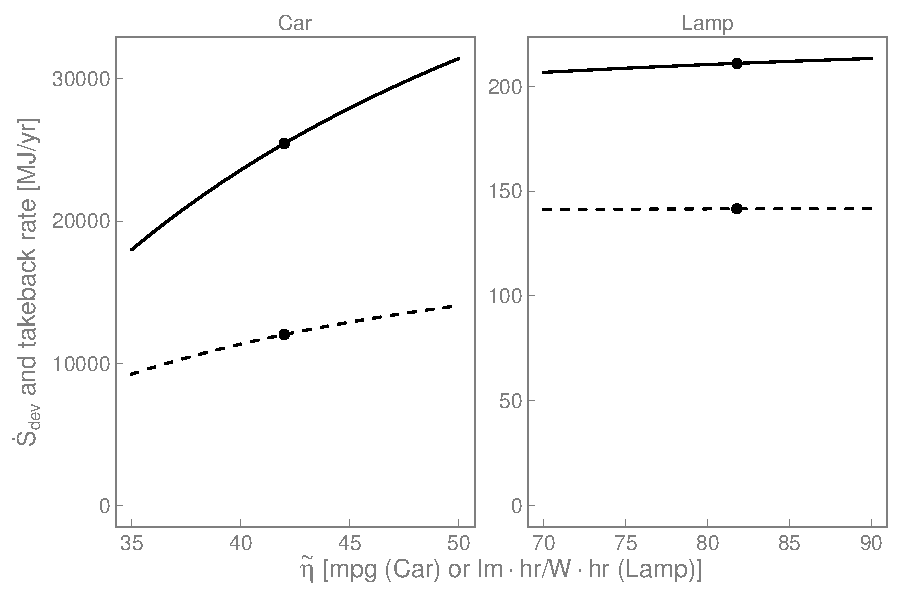
\includegraphics[width=\maxwidth]{figure/eta_tilde_takeback_Sdot_sens_graph-1} 

}

\caption[Expected energy savings rate ($\Sdot$, solid line) and takeback rate (dashed line) sensitivity to post-EEU efficiency ($\amacro{\eta}$)]{Expected energy savings rate ($\Sdot$, solid line) and takeback rate (dashed line) sensitivity to post-EEU efficiency ($\amacro{\eta}$). The macro factor is set to its calibrated value ($k = 3$). (Note different $x$- and $y$-axis scales.)}\label{fig:eta_tilde_takeback_Sdot_sens_graph}
\end{figure}

\end{knitrout}
  
  
Saturation can be seen mathematically, too.
Taking the limit as $\amacro{\eta} \rightarrow \infty$ 
in Eq.~(\ref{PartI-eq:Sdot}) of Part~I gives $\Sdot = \rbempl{E}_s$, 
not $\infty$. 
Thus, efficiency saturation must occur.
Fig.~\ref{fig:eta_tilde_takeback_Sdot_sens_graph}
shows that this framework correctly replicates
expected efficiency saturation trends.

Saturation is especially noticeable in the lamp example
compared to the car example,
the difference being that 
the LED lamp is already much more efficient than the incandescent lamp
(9.26$\times$),
whereas the hybrid car is only 
1.68$\times$ more efficient than the conventional gasoline car. 
Thus, at $\amacro{\eta} = 81.8$ \lmhr/\Whr, 
the energy efficient LED
is far closer to efficiency saturation than the hybrid vehicle 
(at $\amacro{\eta} = 42$ mpg).
As a result, further increases in the LED lamp's efficiency 
are less effective than further increases in the hybrid car's efficiency.

That said, actual savings is the difference between the expected energy savings line (solid line)
and the takeback line (dashed line) in Fig.~\ref{fig:eta_tilde_takeback_Sdot_sens_graph}.
Because the gap between the lines grows, 
higher efficiency yields greater energy savings,
even after accounting for rebound effects.
But the actual savings are always less than expected savings, due to takeback.

Fig.~\ref{fig:eta_tilde_takeback_Sdot_sens_graph} shows that
expected energy savings ($\Sdot$) increase faster than takeback 
as $\amacro{\eta}$ increases.
Thus, total rebound ($Re_{tot}$, the ratio of 
takeback rate to expected energy savings rate in Eq.~(\ref{PartI-eq:Re_takeback}) of Part~I),
decreases as efficiency grows.
The lamp exhibits a relatively smaller rebound decline with efficiency,
because the lamp example is closer to saturation than the car example.

Fig.~\ref{fig:all_Re_terms_eta_graph} shows the variation of all rebound components
with post-EEU efficiency ($\amacro{\eta}$).
In the car and lamp examples, 
direct substitution rebound ($Re_{dsub}$) is the 
rebound component 
most sensitive to changes in post-EEU efficiency ($\amacro{\eta}$).

% A limitation of the energy efficiency sensitivity analysis is that 
% post-EEU efficiency ($\amacro{\eta}$)
% is unlikely to be independent of other factors, 
% such as capital cost ($\amacro{C}_{cap}$).

Note that the sensitivity analysis on post-upgrade efficiency 
($\amacro{\eta}$, Fig.~\ref{fig:all_Re_terms_eta_graph})
is the only sensitivity analysis that requires careful explication
of both the numerator and denominator of Eq.~(\ref{PartI-eq:Re_takeback}) in Part~I,
as in Fig.~\ref{fig:eta_tilde_takeback_Sdot_sens_graph}, 
because both the numerator and denominator of Eq.~(\ref{PartI-eq:Re_takeback}) in Part~I
change when post-upgrade efficiency ($\amacro{\eta}$) changes.
The denominator of Eq.~(\ref{PartI-eq:Re_takeback}) in Part~I doesn't change for
the sensitivity analyses of Figs.~\ref{fig:all_Re_terms_C_cap_graph}--\ref{fig:all_Re_terms_k_graph}.
Thus, for the remaining sensitivity analyses, 
when the rebound percentage increases (decreases), 
the energy takeback rate in the numerator of Eq.~(\ref{PartI-eq:Re_takeback}) in Part~I
increases (decreases) proportionally,
and the actual energy savings rate decreases (increases) accordingly.


\begin{knitrout}
\definecolor{shadecolor}{rgb}{0.969, 0.969, 0.969}\color{fgcolor}\begin{kframe}


{\ttfamily\noindent\color{warningcolor}{\#\# Warning: The `legend.text.align` argument of `theme()` is deprecated as of ggplot2\\\#\# 3.5.0.\\\#\# i Please use theme(legend.text = element\_text(hjust)) instead.\\\#\# This warning is displayed once every 8 hours.\\\#\# Call `lifecycle::last\_lifecycle\_warnings()` to see where this warning was\\\#\# generated.}}\end{kframe}\begin{figure}

{\centering 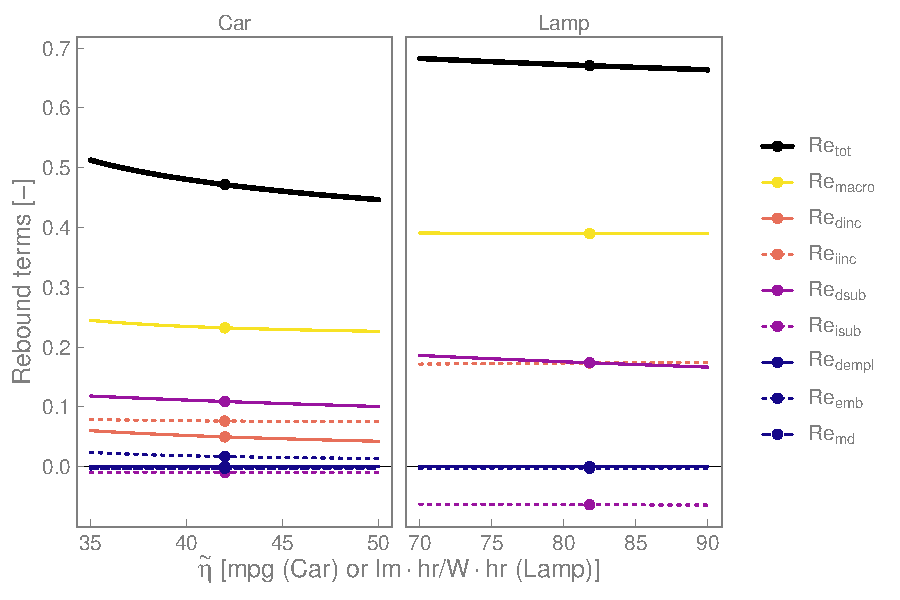
\includegraphics[width=\maxwidth]{figure/all_Re_terms_eta_graph-1} 

}

\caption[Sensitivity of rebound components to post-EEU efficiency ($\amacro{\eta}$)]{Sensitivity of rebound components to post-EEU efficiency ($\amacro{\eta}$). The macro factor is set to its calibrated value ($k = 3$).}\label{fig:all_Re_terms_eta_graph}
\end{figure}

\end{knitrout}


%++++++++++++++++++++++++++++++
\subsection{Effect of capital cost ($\amacro{C}_{cap}$) on rebound terms} 
\label{sec:effect_of_capital_cost}
%++++++++++++++++++++++++++++++

The sensitivity of energy rebound
to capital cost ($\amacro{C}_{cap}$) is shown
in Fig.~\ref{fig:all_Re_terms_C_cap_graph}.
All other things being equal,
as capital cost of the EEU rises, 
less net savings result from the emplacement effect,
leading to smaller income, macro, and total rebound.
The same effects would be observed
with increasing maintenance and disposal cost rate ($\ramacro{C}_{\md}$).

% A limitation of the capital cost sensitivity analysis is that
% capital cost ($\amacro{C}_{cap}$) is unlikely to be
% independent of $\amacro{\eta}$.
% Within a given energy efficiency technology
% (e.g., hybrid cars or LED lamps),
% greater capital cost ($\amacro{C}_{cap}$) may be associated with
% greater service efficiency ($\amacro{\eta}$).
% $\amacro{C}_{cap}$ and $\amacro{\eta}$ should probably be varied jointly,
% not independently.

\begin{knitrout}
\definecolor{shadecolor}{rgb}{0.969, 0.969, 0.969}\color{fgcolor}\begin{figure}

{\centering 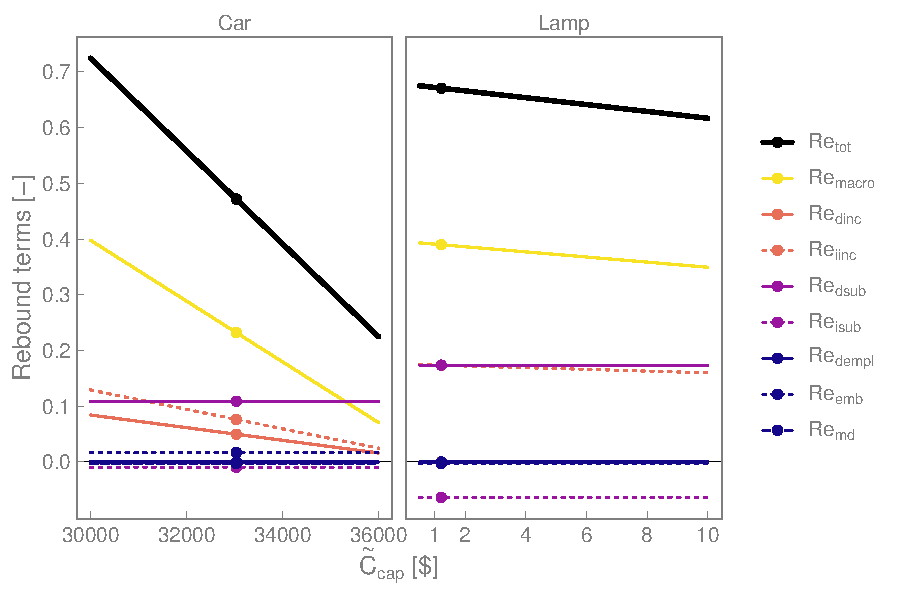
\includegraphics[width=\maxwidth]{figure/all_Re_terms_C_cap_graph-1} 

}

\caption[Sensitivity of rebound components to capital cost ($\amacro{C}_{cap}$)]{Sensitivity of rebound components to capital cost ($\amacro{C}_{cap}$). The macro factor is set to its calibrated value ($k = 3$).}\label{fig:all_Re_terms_C_cap_graph}
\end{figure}

\end{knitrout}


%++++++++++++++++++++++++++++++
\subsection{Effect of energy price ($p_E$) on rebound terms} 
\label{sec:effect_of_energy_price}
%++++++++++++++++++++++++++++++




The effect of energy price on rebound is shown in Fig.~\ref{fig:all_Re_terms_p_E_graph}.
Increasing energy prices lead to larger total rebound ($Re_{tot}$),
because higher energy prices lead to more net savings ($\rasub{N}$)
to be spent by the device user.
All other things being equal, more net savings leads to 
more spending on other goods and services that demand energy.

Fig.~\ref{fig:all_Re_terms_p_E_graph} also 
shows the effect of energy price ($p_E$)
on all rebound components.
Most rebound components increase with energy price, 
with the car and lamp examples exhibiting different sensitivities. 
Substitution effects ($Re_{dsub}$ and $Re_{isub}$)
are the only rebound components that decrease with energy price ($p_E$).
Substitution effects decrease with energy price, because 
at high energy price, less behavior adjustment is needed to re-equilibrate 
after emplacement of the efficient device.



In Fig.~\ref{fig:all_Re_terms_p_E_graph}, German energy prices%
\footnote{
  For the car example,
  the gasoline price in Germany is taken as 1.42 \euro{}/liter for the average ``super gasoline'' (95 octane) 
  price in 2018~\citep{finanzen}.
  For the lamp example,
  the electricity price in Germany is taken as 0.3 \euro{}/\kWhr for the 2018 price of a household using 3.5~MWh/yr,
  an average value for German households~\citep{bundesministerium}.
  Converting currency (at 1 \euro{} = \$1.21) and
  physical units gives 
  6.5~\$/US~gallon and 
  0.363~\$/\kWhr.}
%
are shown as vertical lines,
providing an indication of possible energy price variations.
All other things being equal, 
if U.S.\ residents paid Germany's energy prices,
total energy rebound ($Re_{tot}$) would be 
$84.0$\%
for the car example and 
$148.0$\%
for the lamp example.

% A limitation of the energy price sensitivity analysis arises from the fact that
% energy price is not independent of other parameters.
% Indeed, other rebound parameters
% would change along with energy price
% (especially if moving from one country to another),
% including capital cost ($\amacro{C}_{cap}$), 
% maintenance and disposal expenditure rate ($\ramacro{C}_{\md}$),
% energy intensity of the economy ($I_E$), and
% energy service consumption rate ($\rbempl{q}_s$).

\begin{knitrout}
\definecolor{shadecolor}{rgb}{0.969, 0.969, 0.969}\color{fgcolor}\begin{figure}

{\centering 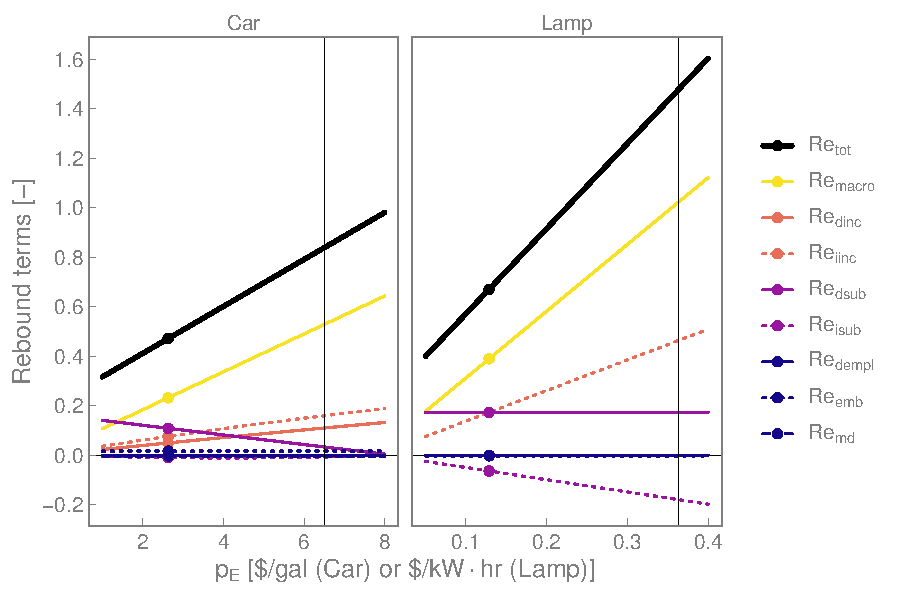
\includegraphics[width=\maxwidth]{figure/all_Re_terms_p_E_graph-1} 

}

\caption[Sensitivity of rebound components to energy price ($p_E$)]{Sensitivity of rebound components to energy price ($p_E$). German energy prices denoted by vertical lines. The macro factor is set to its calibrated value ($k = 3$).}\label{fig:all_Re_terms_p_E_graph}
\end{figure}

\end{knitrout}
  
  
%++++++++++++++++++++++++++++++
\subsection{Effect of original uncompensated own price elasticity ($\eqspsUC^\circ$) on rebound terms} 
\label{sec:effect_of_elasticity}
%++++++++++++++++++++++++++++++



\begin{knitrout}
\definecolor{shadecolor}{rgb}{0.969, 0.969, 0.969}\color{fgcolor}\begin{figure}

{\centering 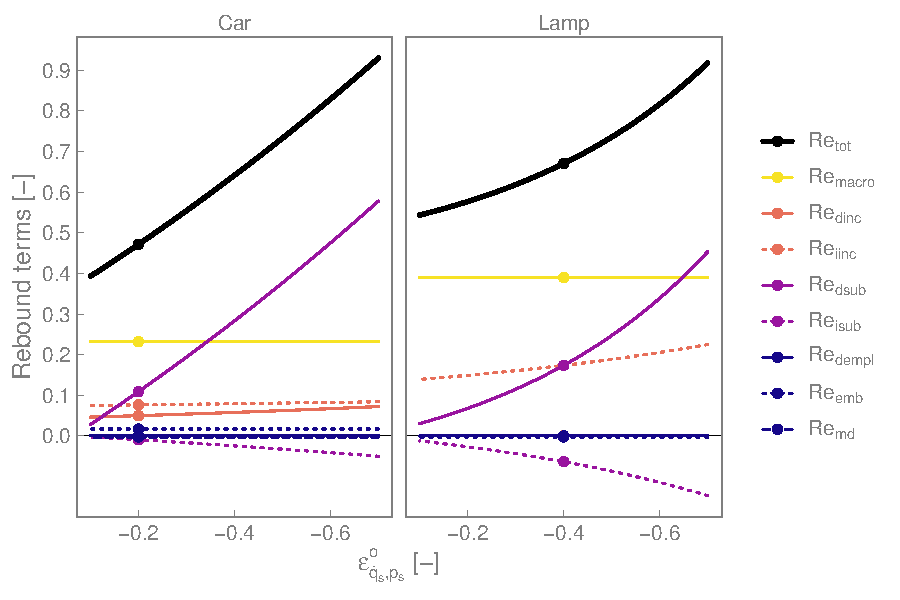
\includegraphics[width=\maxwidth]{figure/all_Re_terms_eps_graph-1} 

}

\caption[Sensitivity of rebound components to uncompensated own price elasticity of energy service demand ($\eqspsUCorig$)]{Sensitivity of rebound components to uncompensated own price elasticity of energy service demand ($\eqspsUCorig$). The macro factor is set to its calibrated value ($k = 3$). (Note reversed $x$-axis scale.)}\label{fig:all_Re_terms_eps_graph}
\end{figure}

\end{knitrout}
  
  


Fig.~\ref{fig:all_Re_terms_eps_graph} shows the variation of total rebound ($Re_{tot}$)
with the original uncompensated price elasticity of energy service demand ($\eqspsUCorig$).
The effect is exponential, and
total rebound increases with larger negative values of $\eqspsUCorig$, as expected.
The lamp example also shows stronger exponential variation than the car example.
The main reason that total rebound values 
are different between the two examples
is the larger absolute value of original uncompensated own price elasticity ($\eqspsUCorig$) 
for the lamp ($-0.4$) compared to the car ($-0.2$).
Were the car to have the same original uncompensated own price elasticity
as the lamp (i.e., $-0.4$), 
total rebound would be closer for both examples 
($64.1$\% for the car and 
$67.1$\% for the lamp).
Fig.~\ref{fig:all_Re_terms_eps_graph} shows that direct substitution rebound 
($Re_{dsub}$) is the most sensitive rebound component to changes in $\eqspsUC^\circ$.
For the lamp example, indirect income rebound ($Re_{iinc}$) also increases
substantially with $\eqspsUC^\circ$, 
because net savings increases substantially with $\eqspsUC^\circ$. 

% A limitation of the elasticity sensitivity study derives from limitations of the 
% CES utility model itself, which constrains price elasticity variation
% given an elasticity of substitution.
% Uneconomic conditions should be avoided.
% For example, negative direct substitution rebound ($Re_{dsub} < 0$)
% is obtained when $\left| \eqspsUC \right| < \fCs$,
% because the elasticity of substitution goes negative ($\sigma < 0$).
% (See Eq.~(\ref{PartI-eq:sigma}) in Appendix~\ref{PartI-sec:utility_and_elasticities} of Part~I.)
% In reality, smaller negative (closer to 0) price elasticity ($\eqspsUC$)
% would correlate with a smaller fraction of expenses spent on the energy service ($\fCs$), 
% thereby avoiding the uneconomic condition.
% However, a univariate sensitivity study cannot capture this effect and is
% best used for smaller variations in $\eqspsUC$
% about a nominal value.

  
%++++++++++++++++++++++++++++++
\subsection{Effect of macro factor ($k$) on rebound terms} 
\label{sec:effect_of_macro_factor}
%++++++++++++++++++++++++++++++

The sensitivity of energy rebound 
to the macro factor ($k$) is shown 
in Fig.~\ref{fig:all_Re_terms_k_graph}.
The macro factor has a linear effect on total rebound ($Re_{tot}$)
through the macro rebound component ($Re_{\macro}$).
All other rebound components are constant when $k$ is varied independently.

% A limitation of the macro factor sensitivity analysis is that
% the macro factor ($k$) is unlikely to be 
% independent of $I_E$, because 
% different values of $k$ imply a different macroeconomy.

\begin{knitrout}
\definecolor{shadecolor}{rgb}{0.969, 0.969, 0.969}\color{fgcolor}\begin{figure}

{\centering 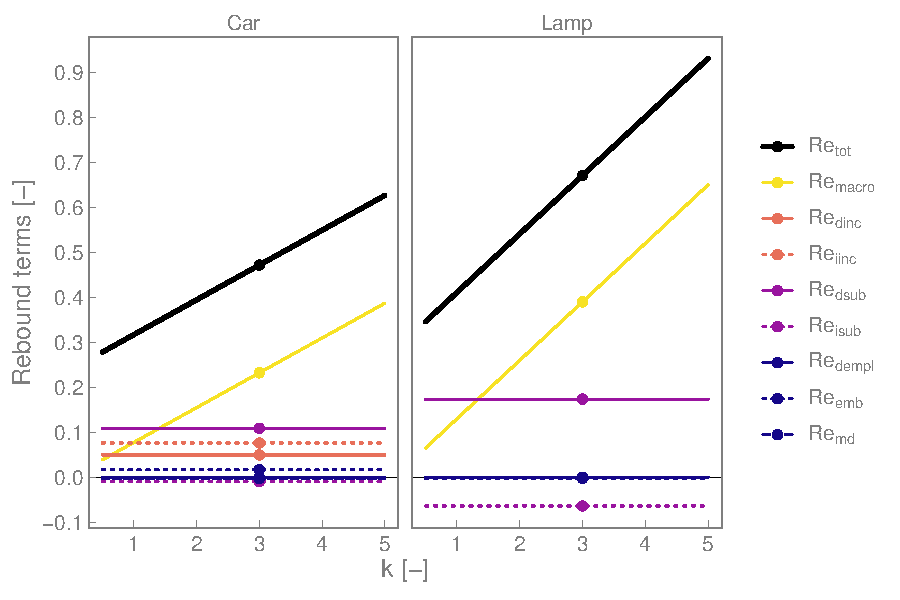
\includegraphics[width=\maxwidth]{figure/all_Re_terms_k_graph-1} 

}

\caption[Sensitivity of rebound components to the macro factor ($k$)]{Sensitivity of rebound components to the macro factor ($k$).}\label{fig:all_Re_terms_k_graph}
\end{figure}

\end{knitrout}
  

%++++++++++++++++++++++++++++++
\subsection{Effect of energy service price ($\amacro{p}_s$) on price elasticities ($\asub{\varepsilon}$)}
\label{sec:price_elasticities_sensitivity}
%++++++++++++++++++++++++++++++

The sensitivity of post-substitution effect price elasticities ($\asub{\varepsilon}$)
to post-upgrade energy service price ($\amacro{p}_s$)
is shown in Fig.~\ref{fig:PriceElasticitySensGraph}
for the CES utility model described 
in Section~\ref{PartI-sec:sub_effect_main_paper} 
and Appendix~\ref{PartI-sec:utility_and_elasticities}
of Part~I.
Note that the left side of each graph ($\amacro{p}_{s} = 0$)
represents unattainable infinite efficiency ($\amacro{\eta}_s \rightarrow \infty$), 
i.e., delivery of the energy service without energy consumption.

First, note the sign of the elasticities. As expected, both of the
uncompensated price elasticities ($\eqspsUChat$ and $\eqopsUChat$,
dashed lines in Fig.~\ref{fig:PriceElasticitySensGraph}) 
are negative, regardless of the energy service price ($\amacro{p}_s$):
a lower price means more consumption of both
goods, all other things being equal.
The compensated own price elasticity ($\eqspsChat$) is negative
and the compensated cross price elasticity ($\eqopsChat$) is positive.
As $\amacro{p}_s$ declines, the consumers substitutes the energy
service for other goods.

\begin{knitrout}
\definecolor{shadecolor}{rgb}{0.969, 0.969, 0.969}\color{fgcolor}\begin{figure}

{\centering 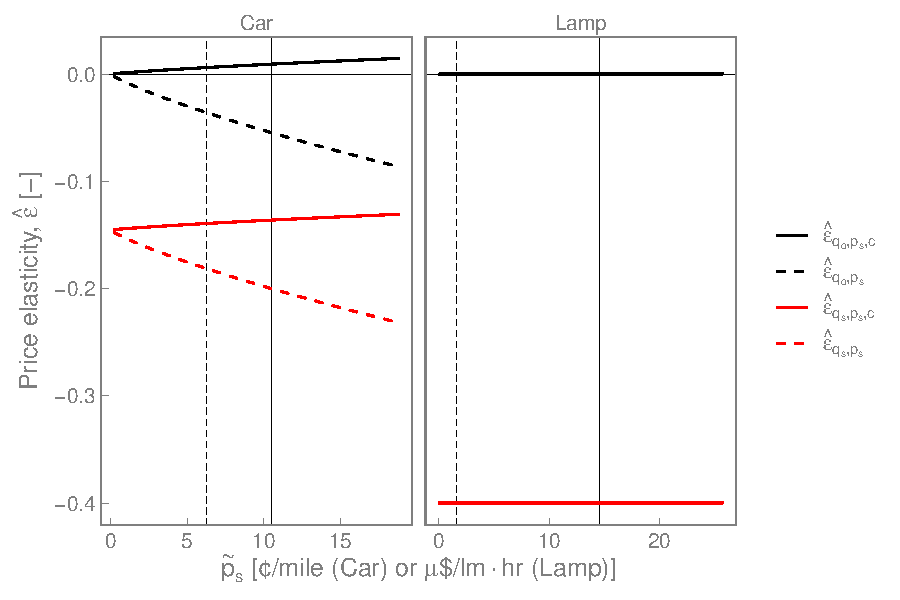
\includegraphics[width=\maxwidth]{figure/PriceElasticitySensGraph-1} 

}

\caption{Sensitivity of post substitution effect price elasticities ($\asub{\varepsilon}$) to post-EEU energy service price ($\amacro{p}_{s}$) for the CES utility model. The solid vertical line indicates the original energy service price ($\orig{p}_s$), and the dashed vertical line indicates the upgraded energy service price ($\amacro{p}_s = \ainc{p}_s = \asub{p}_s = \aempl{p}_s$) for the two examples. See Tables~\ref{tab:car_stages_table} and \ref{tab:lamp_stages_table} for $p_s$ in different units.}\label{fig:PriceElasticitySensGraph}
\end{figure}

\end{knitrout}


Second, the magnitude of price elasticities varies.
Fig.~\ref{fig:PriceElasticitySensGraph} shows that the car example exhibits
more variation of price elasticities ($\asub{\varepsilon}$) with energy service price ($\amacro{p}_s$)
than the lamp example, 
because the expenditure share ($\fCs$) for the lamp example is very small
compared to the car example.
Using the constant price elasticity (CPE) utility model may be a
good enough approximation in the lamp example. 
However, for the car example, using the CES utility function will be necessary
to eliminate errors that will be present in the CPE approximation.
This result is an important finding that should encourage 
analysts implementing analytical rebound calculations
with substitution and income effects
to prefer the CES utility model over the CPE approximation.

Fig.~\ref{fig:PriceElasticitySensGraph} shows that
as efficiency increases (and $\amacro{p}_s$ decreases), 
the absolute value of the uncompensated price elasticities 
($\eqspsUChat$ and $\eqopsUChat$) decreases, 
a change that exceeds the slightly increasing (in absolute value terms)
compensated own price elasticity ($\eqspsChat$). 
Thus, direct rebound is attenuated as efficiency increases,
relative to a constant price elasticity model.
(See also the patterns of lines of Fig.~\ref{fig:all_Re_terms_eta_graph},
which show a declining trend.)


\end{document}
